\documentclass[11pt,a4paper]{article}
\usepackage[T1]{fontenc}
\usepackage[utf8]{inputenc}
\usepackage{lmodern}
\usepackage{amsmath,amssymb,amsthm,mathtools}
\usepackage[margin=27mm]{geometry}
\usepackage{microtype,booktabs,array,graphicx,xcolor,tabularx}
\usepackage{tikz}
\usetikzlibrary{arrows.meta,bending}
\usepackage{enumitem}
\usepackage[numbers,sort&compress]{natbib}
\usepackage{hyperref}
\usepackage{fancyhdr}
\definecolor{plum}{HTML}{6C3569}
\definecolor{teal}{HTML}{367E78}
\definecolor{ochre}{HTML}{AE8238}
\hypersetup{colorlinks=true,linkcolor=plum,citecolor=plum,urlcolor=teal,
 pdftitle={Smoothness within and across Wardrop route regimes},pdfauthor={Anonymous}}
\pagestyle{fancy}
\fancyhf{}
\fancyhead[L]{\small Smoothness within and across Wardrop route regimes}
\fancyhead[R]{\small Anonymous}
\fancyfoot[C]{\thepage}
\setlength{\headheight}{14pt}
\setlength{\parskip}{3pt}
\setlength{\emergencystretch}{2em}
\newtheorem{theorem}{Theorem}[section]
\newtheorem{proposition}[theorem]{Proposition}
\newtheorem{lemma}[theorem]{Lemma}
\newtheorem{corollary}[theorem]{Corollary}
\theoremstyle{definition}
\newtheorem{definition}[theorem]{Definition}
\newtheorem{example}[theorem]{Example}
\theoremstyle{remark}
\newtheorem{remark}[theorem]{Remark}
\newcommand{\R}{\mathbb R}
\newcommand{\PoA}{\operatorname{PoA}}
\newcommand{\eq}{\mathrm{eq}}
\newcommand{\opt}{\mathrm{opt}}
\newcommand{\dd}{\,\mathrm d}
\newcommand{\Kc}{\mathcal K}
\newcommand{\Fs}{\mathcal F}
\newcommand{\status}[1]{\textsf{\small[#1]}}
\DeclareMathOperator{\diag}{diag}
\DeclareMathOperator{\sgn}{sgn}

\title{Smoothness within and across\\Wardrop route regimes}
\author{Anonymous}
\date{22 October 2026}

\begin{document}
\maketitle
\vspace{-1.5em}
\begin{abstract}
Cominetti, Dose and Scarsini (2024) left two questions open about how Wardrop equilibria respond to demand. First, does equilibrium remain continuously differentiable along a demand path, while the set of cheapest routes stays fixed, when link costs have zero slope at zero load, as Bureau of Public Roads (BPR) costs do? We prove that it does at every interior demand level, with no restriction on the network. Second, when a new route becomes cheapest, must the slope of total travel cost or of the price of anarchy jump? We show that it need not. A five-link network with standard quartic BPR costs has a genuine route expansion at which total cost and the price of anarchy have four continuous derivatives. Five links are the fewest possible for common-exponent BPR costs, for route expansions and contractions alike. The slope can never jump in the wrong direction, even with zero free-flow times. For almost every choice of free-flow times it does jump, at least wherever the smaller set of cheapest routes uses only loaded links. So a regime change with no kink is possible but exceptional. In practice, a route that becomes active this way carries too little flow for an assignment run at ordinary convergence tolerances to resolve.
\end{abstract}
\noindent\textbf{Keywords:} Wardrop equilibrium; traffic assignment; BPR cost functions; price of anarchy; sensitivity analysis; route-set changes.\\
\textbf{2020 Mathematics Subject Classification:} 90B20, 91A14, 91A43, 90C31.\quad
\textbf{JEL:} C61, C72, R41.

\section{Introduction}\label{sec:intro}

\subsection{Two questions}

In a static traffic assignment every traveller uses a cheapest route, and as demand grows the set of cheapest routes changes from time to time. Cominetti, Dose and Scarsini \cite{CDS2024} (hereafter CDS) studied how total equilibrium travel time and the price of anarchy behave as demand is scaled. They proved that these quantities are continuously differentiable while the set of cheapest routes stays fixed, provided every link cost has a strictly positive slope. They also proved that at a change in the set of cheapest routes the slope moves in a predictable direction. Two questions remained open. We quote them from the arXiv version of their paper (v2), whose numbering we follow throughout.

\textbf{Question 1.} Their Theorem~3.2 is the fixed-regime smoothness theorem. In the paragraph after their Remark~3.5, which introduces their Examples~3.6 and~3.7, they write:
\begin{quote}
``Whether Theorem 3.2 can be extended to cost functions that exhibit a zero derivative only at the origin remains an open problem.''
\end{quote}
BPR costs $a(1+0.15(z/C)^4)$ have exactly this feature: their slope is zero at zero load and positive elsewhere.

\textbf{Question 2.} Their Theorem~4.4(ii) shows that for affine costs the slope of total cost and of the price of anarchy changes strictly at every breakpoint whose two regimes are nested. In the paragraph preceding their Example~4.9 they write:
\begin{quote}
``It is an open question whether this is also the case for convex costs or BPR costs.''
\end{quote}
Section~\ref{sec:background} restates the relevant results of CDS, so the reader need not have their paper at hand.

\subsection{Answers in brief}

\textbf{Answer to Question 1: yes, at interior points} (Theorem~\ref{fr:theorem}). If every link cost is continuously differentiable with positive slope at positive load, then along any continuously differentiable demand path the equilibrium link flows are continuously differentiable on every open interval on which the set of cheapest routes is constant. The slope may vanish at zero load, and the zero-load links may form cycles. Free-flow times may be zero, demands may vanish, route sets may be restricted, and different links may have different BPR exponents. CDS's theorem also allows the end point $t_0=0$. There the extension fails in general (Proposition~\ref{fr:endpoint}), although our counterexample does not use BPR costs. Whether it fails for BPR costs at zero demand is open.

\textbf{Answer to Question 2: no.} Strictness can fail for BPR costs and for strictly convex costs.
\begin{itemize}[nosep]
\item Three links suffice: one example has strictly convex polynomial costs, and another has BPR-type costs with different exponents and a contraction (Section~\ref{sec:smallexamples}).
\item With the standard common quartic exponent, a five-link network has a genuine expansion of the set of cheapest routes. Total cost $E$ and the price of anarchy $P$ have four continuous derivatives there, and their fifth derivatives jump (Section~\ref{sec:fiveedge}).
\item Five links are the minimum in the common-exponent class, for expansions and for contractions (Theorem~\ref{thm:minimal}).
\item More links allow any finite number of matching derivatives (Theorem~\ref{thm:main}).
\end{itemize}

Three further results put the negative answer in proportion.
\begin{enumerate}[nosep]
\item \emph{The slope never jumps in the wrong direction} (Theorem~\ref{thm:weakcomparison}). The weak inequalities of CDS Theorem~4.4(i) hold for BPR costs, both at expansions and at contractions, even with zero free-flow times. CDS Remark~4.6 names exactly this extension as the consequence an answer to Question~1 would bring.
\item \emph{A missing jump is exceptional} (Theorem~\ref{thm:generic}). For almost every vector of free-flow times, every nested breakpoint at which the smaller regime uses only loaded links has a strict slope jump.
\item \emph{The price of anarchy has a second hidden transition} (Theorem~\ref{thm:optimumtransition}). In the common-power examples the system optimum changes its route set earlier, at $t=1/\gamma$. There the price of anarchy is even smoother: five continuous derivatives in the quartic example.
\end{enumerate}

\subsection{The main idea}\label{sec:mainidea}

Figure~\ref{fig:idea} shows the mechanism. Two groups of parallel links (``banks'') serve two commodities. A connector link lets commodity A switch from its own bank to the other bank. The connector is worth using when the \emph{route gap}
\[
\Delta(t)=\text{(cost of A's direct route)}-\text{(cost of the connector route)},
\]
computed without connector flow, becomes positive. Usually $\Delta$ crosses zero with nonzero slope. The connector flow then grows linearly in $t-1$, and the slope of total cost jumps. If instead the two bank delay curves touch to order $m$, then $\Delta(t)\approx a(t-1)^m$. Each extra link in a bank supplies one extra free coefficient, and $m+1$ bank links can make the first $m-1$ derivatives of the two delay curves agree.

Two orders then add. The connector flow is $x\approx\Delta/L_0$, of order $m$, where $L_0$ is the curvature of the switching cost. To first order the change in total cost is the flow moved times the rate at which the gap opens:
\[
E-E_0\approx -t\,\Delta'(t)\,x,
\]
of order $(m-1)+m=2m-1$. Here $E_0$ is the cost the network would have without the connector. The connector itself is invisible to first order, because travellers switch only when the two routes cost the same. With the smallest odd order $m=3$, the cost difference is of order $(t-1)^5$, so $E$ has four continuous derivatives. In potential terms, the Beckmann potential changes by $-\Delta^2/(2L_0)$, of order $2m$, and $E=tV'$ loses one order (Remark~\ref{rem:potential}).

\begin{figure}[htbp]
\centering
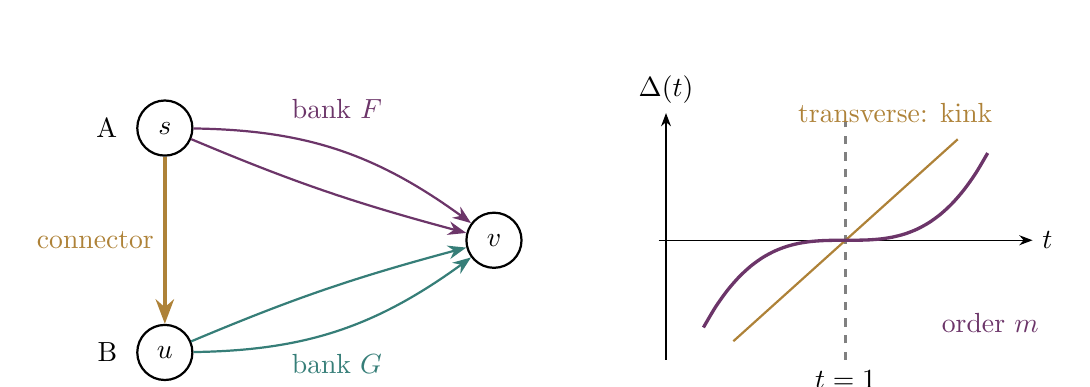
\begin{tikzpicture}[>=Stealth,thick,scale=0.95]
\begin{scope}
\node[circle,draw,minimum size=7mm] (s) at (0,1.9) {$s$};
\node[circle,draw,minimum size=7mm] (u) at (0,-1.1) {$u$};
\node[circle,draw,minimum size=7mm] (v) at (4.4,0.4) {$v$};
\draw[->,plum] (s) to[bend left=18] (v);
\draw[->,plum] (s) to[bend right=4] (v);
\draw[->,teal] (u) to[bend left=4] (v);
\draw[->,teal] (u) to[bend right=18] (v);
\draw[->,ochre,line width=1.3pt] (s) -- node[left] {connector} (u);
\node[plum] at (2.3,2.15) {bank $F$};
\node[teal] at (2.3,-1.25) {bank $G$};
\node[anchor=east] at (-0.5,1.9) {A};
\node[anchor=east] at (-0.5,-1.1) {B};
\end{scope}
\begin{scope}[xshift=6.6cm,yshift=-1.2cm]
\draw[->,thin] (0,1.6) -- (5.0,1.6) node[right] {$t$};
\draw[->,thin] (0.1,0) -- (0.1,3.3) node[above] {$\Delta(t)$};
\draw[dashed,gray] (2.5,0) -- (2.5,3.2);
\node[below] at (2.5,0) {$t=1$};
\draw[domain=1.0:4.0,smooth,variable=\x,ochre] plot ({\x},{1.6+0.9*(\x-2.5)});
\draw[domain=0.6:4.4,smooth,variable=\x,plum,line width=1.2pt] plot ({\x},{1.6+0.17*(\x-2.5)^3});
\node[ochre,anchor=east] at (4.6,3.3) {transverse: kink};
\node[plum,anchor=west] at (3.65,0.5) {order $m$};
\end{scope}
\end{tikzpicture}
\caption{The two-bank architecture (left) and the route gap $\Delta(t)$ of the connector route (right). With a transverse crossing the connector flow grows linearly and the slope of total cost jumps. If the bank delay curves touch to order $m$, the gap vanishes to order $m$, the connector flow grows like $(t-1)^m$ and total cost differs by order $(t-1)^{2m-1}$.}
\label{fig:idea}
\end{figure}

\subsection{Results at a glance}

Table~\ref{tab:glance} lists the main results, their status and where they are proved. Throughout, ``proof'' means a complete analytic proof in this paper. ``Exact'' means a computation in rational arithmetic, used only to confirm constants. ``Numerical'' means a floating-point computation, and ``exploratory'' means an illustration without a claim of generality.

\begin{table}[htbp]
\centering\small
\begin{tabularx}{\linewidth}{@{}>{\raggedright\arraybackslash}p{3.6cm}>{\raggedright\arraybackslash}X>{\raggedright\arraybackslash}p{2.2cm}l@{}}
\toprule
Topic & Result & Status & Where\\
\midrule
Question 1 & Fixed-regime $C^1$ link flows for costs with $c'(z)>0$ for $z>0$; $S$ and $P$ are $C^1$ & proof & Thm~\ref{fr:theorem}\\
Endpoint & General one-sided extension at $t_0=0$ fails; BPR endpoint case open & proof; open & Prop.~\ref{fr:endpoint}\\
Weak comparison & CDS Thm~4.4(i) holds for BPR costs, expansions and contractions, zero free-flow allowed & proof & Thm~\ref{thm:weakcomparison}\\
Genericity & Strict jumps for almost every free-flow vector at nondegenerate nested breakpoints & proof & Thm~\ref{thm:generic}\\
Question 2, convex & Three-link polynomial triangle with $E,P\in C^4\setminus C^5$ & proof; exact & \S\ref{sec:smallexamples}\\
Question 2, BPR & Five-link common-quartic expansion with $E,P\in C^4\setminus C^5$ & proof; exact & \S\ref{sec:fiveedge}\\
Any finite order & $m+2$ links, $E,P\in C^{2m-2}\setminus C^{2m-1}$, every $p>1$ & proof & Thm~\ref{thm:main}\\
Minimality & Common power: five links minimal for expansions and contractions; mixed powers: contractions need three, expansions four or five (open) & proof; open & Thm~\ref{thm:minimal}\\
Optimum side & $S\in C^{2m-1}\setminus C^{2m}$ at $t=1/\gamma$; same for $P$ when $E$ is $C^{2m}$ there, checked for the quartic example; jump $\approx+89.7$ & proof; exact check; numerical value & Thm~\ref{thm:optimumtransition}\\
Robustness & Kinks return under perturbation, at size $|\varepsilon|^{2-2/m}$; transverse demand directions give $C^1\setminus C^2$ & proof & \S\ref{sec:robustness}\\
Practice & Hidden activation below assignment tolerance; link flows reveal it earlier & numerical & \S\ref{sec:practice}\\
Sioux Falls & Link activations along a demand scaling are transverse with visible kinks & exploratory & \S\ref{sec:sioux}\\
Several contacts & Sharp contact budget and synthesis of prescribed transitions in the two-bank architecture & proof; exact & App.~\ref{app:contacts}\\
\bottomrule
\end{tabularx}
\caption{Results at a glance.}
\label{tab:glance}
\end{table}

\subsection{Related work}

\emph{Demand dependence of the price of anarchy.} O'Hare, Connors and Watling \cite{OCW2016} studied how the price of anarchy varies with demand and conjectured the slope inequalities that CDS proved in a restricted form. They also proved the flow scaling between equilibrium and optimum for common-power costs, which we use. Light- and heavy-traffic limits are studied in \cite{CB2020,CB2019,WuMohring2021}, demand sensitivity of the price of anarchy in \cite{WuMohring2023,Englert2010}, and empirical demand curves in \cite{Youn2008,Monnot2017}. CDS also treat the single-commodity case in \cite{CDSMP}. Dose \cite{Dose2026} studies efficient demand levels in two-link networks.

\emph{Sensitivity of traffic equilibria.} Hall \cite{Hall1978} showed that equilibrium flows depend continuously on demand but need not be differentiable. Directional differentiability and sensitivity formulas under strict monotonicity or nondegeneracy were developed by Dafermos and Nagurney \cite{DafermosNagurney1984,Dafermos1988}, Tobin and Friesz \cite{TobinFriesz1988}, Qiu and Magnanti \cite{QiuMagnanti1989}, Patriksson \cite{Patriksson2004}, Josefsson and Patriksson \cite{JP2007} and Lu \cite{Lu2008}. These results describe directional derivatives at a given demand, typically under strictly increasing costs. They do not give continuity of the derivative along a path on which some links have zero load and zero cost slope and those links form cycles. That degenerate case is the content of Question~1, and CDS Remark~3.5(b) covers it only when the zero-slope links contain no undirected cycle. Our proof replaces the nondegeneracy assumption by a uniform bound for weighted least-squares problems \cite{Stewart1989,Forsgren1996}.

\emph{Recent work.} Wang, Shao and Wu \cite{WSW2026} prove, for continuous nondecreasing costs, that the Beckmann value function is continuously differentiable on the open positive demand cone. They deduce that equilibrium total cost and the price of anarchy are continuously differentiable on the interior of every region of demand space with a fixed positive-flow support, with no condition on cost slopes. This overlaps our conclusion that $E$ and $P$ are $C^1$. Their cellwise smoothness of edge costs and loads (their Theorem~3) assumes costs with positive slope everywhere, or constant costs, and so excludes BPR costs, whose slope vanishes at zero load. Their results also concern full-dimensional interiors of demand regions, so they do not cover demand curves that run along the boundary between two regions (CDS Remark~3.5(a)) or demands that vanish. They also show that the set where the price of anarchy is not differentiable has measure zero in demand space. Our genericity theorem is of a different kind: it concerns the size of the slope jump at a breakpoint, for almost every free-flow vector. D'Ambrosio \cite{DAmbrosio2026} gives a quartic BPR network with an interior local maximum of the price of anarchy while the active network is constant. That concerns the shape of the price of anarchy, not slope equality at breakpoints.

\emph{Classical ingredients.} We use the Beckmann potential \cite{BMW1956}, the envelope theorem in Danskin's form \cite{Danskin1966}, Sard's theorem \cite{Sard1942}, weighted least-squares bounds \cite{Stewart1989,Forsgren1996}, finite differences and Chebyshev systems \cite{GLT2012,Karlin1968,deBoor2005,BT2004}, and the log-oscillating construction of \cite{CB2020}. Loss of strict complementarity in one-parameter optimisation is studied by Jongen, Jonker and Twilt \cite{JongenJonkerTwilt1986}; there it generically produces a kink, which agrees with Theorem~\ref{thm:generic}.

\subsection{Roadmap}

Section~\ref{sec:background} sets up the model, restates the CDS results and gives a notation dictionary. Section~\ref{fr:section} answers Question~1. Section~\ref{sec:comparison} proves the weak slope comparison for BPR costs and the genericity theorem. Section~\ref{sec:transitions} answers Question~2 with the small examples, the five-link example and the general family. Section~\ref{sec:minimal} gives the minimum link counts. Section~\ref{sec:robustness} shows how kinks return under perturbation and studies the optimum-side transition. Section~\ref{sec:practice} discusses what the results mean for assignment practice, including a Sioux Falls illustration. Section~\ref{sec:conclusion} concludes with open problems. The appendices contain the theory of several contacts, the full proof of the minimality theorem, codimension and infinitely smooth examples, and a guide to the verification code.

\section{Model, background and notation}\label{sec:background}

\subsection{Routing games with variable demand}

A \emph{network} is a finite directed multigraph with edge set $\mathcal E$. Each edge $e$ has a continuous nondecreasing cost $c_e:[0,\infty)\to[0,\infty)$. A \emph{commodity} $k$ has an origin, a destination and a finite nonempty set $\mathcal P_k$ of simple paths (its \emph{routes}). The route sets may be smaller than the set of all paths. For a demand vector $\mu=(\mu_k)\in[0,\infty)^K$, the \emph{feasible set} is
\[
 \Fs(\mu)=\Bigl\{f=(f_{P})\ge0:\ \sum_{P\in\mathcal P_k}f_{P}=\mu_k\ \text{for every }k\Bigr\},
\]
and $f$ induces the edge load $z_e(f)=\sum_k\sum_{P\in\mathcal P_k\colon e\in P}f_P$. Write $\mathcal Z(\mu)=\{z(f):f\in\Fs(\mu)\}$ for the compact convex set of feasible loads. The cost of a route is $c_P(z)=\sum_{e\in P}c_e(z_e)$.

A feasible $f$ is a \emph{Wardrop equilibrium} if every route with $f_P>0$ has minimum cost among the routes of its commodity. Equilibrium loads are the minimisers over $\mathcal Z(\mu)$ of the Beckmann potential $\sum_e\int_0^{z_e}c_e$ \cite{BMW1956,Wardrop1952}. When every $c_e$ is strictly increasing, the equilibrium load $z^\eq(\mu)$ is unique, although the route flows need not be.

\begin{definition}[Complete minimum-route regime]\label{def:regime}
For a load vector $z$ and commodity $k$ put
\[
 R_k(z)=\Bigl\{P\in\mathcal P_k:\ c_P(z)=\min_{Q\in\mathcal P_k}c_Q(z)\Bigr\}.
\]
The \emph{regime} at demand $\mu$ is the family $R(\mu)=(R_k(z^\eq(\mu)))_k$. It depends only on the unique equilibrium load, not on any route decomposition, and it is defined also for commodities with $\mu_k=0$. It contains every cheapest route, used or not. This is the \emph{active regime} of CDS \cite[Definition~2.2]{CDS2024}.
\end{definition}

For a regime $R$, let $\Kc_R$ be the span of the vectors $1_P-1_Q$ with $P,Q\in R_k$ for some $k$, where $1_P$ is the edge-incidence vector of $P$. Equivalently, $\Kc_R$ is the set of edge-load changes produced by signed route flows on $R$ that leave every commodity demand unchanged. At an equilibrium with regime $R$, all routes in $R_k$ have the same cost, so the edge-cost vector satisfies $c(z)\perp\Kc_R$.

Along a demand path $t\mapsto\mu(t)$ we study
\begin{equation}\label{eq:objectives}
 E(t)=\sum_e z^\eq_e c_e(z^\eq_e),\qquad
 S(t)=\min_{z\in\mathcal Z(\mu(t))}\sum_e z_e c_e(z_e),\qquad
 P(t)=\frac{E(t)}{S(t)}.
\end{equation}
These are the equilibrium total cost, the optimal total cost and the price of anarchy. The equilibrium and the optimum are taken over the \emph{same} feasible set $\mathcal Z(\mu(t))$, with the same route sets. In the explicit constructions every simple path is a route, so this set is the set of all loads of the physical network. The examples use the proportional path $\mu(t)=tr$ with a fixed $r$, and $t$ is a dimensionless demand multiplier.

\begin{definition}[Breakpoints]\label{def:breakpoint}
A point $t_0>0$ is a \emph{breakpoint} if the regime is constant, equal to $R_-$, on $(t_0-\varepsilon,t_0)$, constant, equal to $R_+$, on $(t_0,t_0+\varepsilon)$, and $R_-\ne R_+$ (CDS Definition~4.1). These two open intervals are the \emph{punctured sides} of $t_0$. The breakpoint is an \emph{expansion} if $R_-\subsetneq R_+$ and a \emph{contraction} if $R_+\subsetneq R_-$. We write $R_s$ and $R_l$ for the smaller and the larger of the two regimes.
\end{definition}

\subsection{The results of Cominetti, Dose and Scarsini}

We restate the results that the two questions concern, in the present notation.

\emph{CDS Theorem 3.2 (fixed-regime smoothness).} Let the demand $\mu(\cdot)$ be continuously differentiable and let every $c_e$ be $C^1$ with $c_e'>0$ everywhere. If the regime is constant on a neighbourhood of $t_0\ge0$, then (a) the equilibrium loads are $C^1$ near $t_0$, and so are the commodity costs and $E$; (b) if moreover every $z\mapsto zc_e(z)$ is convex, then $S$ and $P$ are $C^1$ near $t_0$. CDS Remark~3.5(b) weakens $c_e'>0$ to strictly increasing costs provided the edges with $c_e'(z_e)=0$ contain no undirected cycle.

\emph{The O'Hare et al.\ conjecture} (CDS Conjecture~4.2, summarising \cite[Conjectures 4.5, 4.6, 4.9]{OCW2016}). Let costs be differentiable and strictly increasing with positive second derivative, let the demand be piecewise affine and nondecreasing, and let $t_0$ be a breakpoint. (a) If $R_-\subset R_+$, then $E'(t_0^-)>E'(t_0^+)$ and $P'(t_0^-)>P'(t_0^+)$. (b) If $R_-\supset R_+$, then $E'(t_0^-)<E'(t_0^+)$ and $P'(t_0^-)<P'(t_0^+)$. CDS Example~4.3 shows that the conjecture fails in this generality.

\emph{CDS Theorem 4.4.} Let $\mu(t)=tr$. (i) If the costs are $C^1$ with $c_e'>0$, the inequalities (a) and (b) hold weakly at every breakpoint. (ii) If the costs are nondecreasing and affine, they hold strictly. CDS Remark~4.6 notes that part (i) excludes BPR costs. It adds that part~(i) would extend to BPR costs given an extension of Theorem~3.2(a) of the kind asked for in Question~1.

So Question~2 asks whether Theorem~4.4(ii) extends from affine to convex or BPR costs.

\subsection{Two value-function facts}

The next proposition handles the optimum for any demand path, with zero demands and restricted route sets. It replaces the appeal to CDS Lemma~3.4 and makes the price-of-anarchy conclusions self-contained. It is an instance of Danskin's envelope theorem \cite{Danskin1966}, and we include the short proof.

\begin{proposition}[Envelope formula for value functions]\label{prop:Sregular}
Let each $g_e:[0,\infty)\to\R$ be convex and $C^1$ with $g_e'$ strictly increasing. Let $\mu:I\to[0,\infty)^K$ be $C^1$ on an open interval $I$, and put
\[
 W(t)=\min_{z\in\mathcal Z(\mu(t))}\sum_eg_e(z_e).
\]
Then the minimising load $z^*(t)$ is unique and continuous, and $W$ is $C^1$ on $I$ with
\begin{equation}\label{eq:envelope}
 W'(t)=\sum_k\mu_k'(t)\,m_k(t),\qquad m_k(t)=\min_{P\in\mathcal P_k}\sum_{e\in P}g_e'(z^*_e(t)).
\end{equation}
In particular $S$ is $C^1$ when every $c_e$ is $C^1$ and every $zc_e(z)$ is \emph{strictly} convex, that is, $c_e+zc_e'$ is strictly increasing. Convexity alone is not enough for uniqueness of the optimal load: with $c(z)=z$ on $[0,1]$ and $c(z)=2-1/z$ for $z\ge1$, two identical parallel links and demand $3$, every split with link loads in $[1,2]$ is optimal. BPR costs $a+bz^p$ with $b>0$, $p\ge1$ satisfy the strict condition. Taking $g_e=\int_0^zc_e$, the Beckmann value $V(t)$ is $C^1$ with $V'=\sum_k\mu_k'\pi_k$, where $\pi_k$ is the equilibrium cost of commodity $k$. On a proportional path $\mu=tr$ this gives $E(t)=tV'(t)$.
\end{proposition}
\begin{proof}
Strict convexity of $\sum_eg_e$ gives a unique minimiser, and compactness gives its continuity in $t$. Write every feasible route flow as $f_P=\mu_k\lambda_P$ with $\lambda_k=(\lambda_P)_{P\in\mathcal P_k}$ in the probability simplex $\Lambda_k$. Put $\Lambda=\prod_k\Lambda_k$ and $\Phi(t,\lambda)=\sum_eg_e(z_e(t,\lambda))$, where $z_e(t,\lambda)=\sum_k\mu_k(t)\sum_{P\ni e}\lambda_P$. Then $W(t)=\min_{\lambda\in\Lambda}\Phi(t,\lambda)$, and
\[
 \partial_t\Phi(t,\lambda)=\sum_k\mu_k'(t)\sum_{P\in\mathcal P_k}\lambda_P\,\sum_{e\in P}g_e'(z_e(t,\lambda)),
\]
which is jointly continuous. Let $\Lambda^*(t)$ be the set of minimisers. For $\lambda\in\Lambda^*(t)$ the load is $z^*(t)$. If $\mu_k(t)>0$, optimality forces $\lambda_P=0$ unless $P$ has minimum marginal cost, so the $k$-th inner sum equals $m_k(t)$. If $\mu_k(t)=0$, then $\mu_k'(t)=0$ because $\mu_k\ge0$ is $C^1$ and $t$ is interior. Hence $\partial_t\Phi(t,\lambda)$ equals the right side of \eqref{eq:envelope} for every $\lambda\in\Lambda^*(t)$.

For $h\ne0$ small, $W(t+h)\le\Phi(t+h,\lambda^*)$ for any $\lambda^*\in\Lambda^*(t)$. If $\lambda_h\in\Lambda^*(t+h)$, then $W(t)\le\Phi(t,\lambda_h)$. The mean value theorem gives
\[
 \partial_t\Phi(t+\theta_hh,\lambda_h)\le\frac{W(t+h)-W(t)}{h}\le\partial_t\Phi(t+\theta'_hh,\lambda^*)\qquad(h>0),
\]
with the inequalities reversed for $h<0$ and $\theta_h,\theta'_h\in(0,1)$. Every limit point of $\lambda_h$ lies in $\Lambda^*(t)$, by continuity. Both bounds therefore tend to the common value \eqref{eq:envelope}. This proves differentiability. The derivative is continuous because $z^*$, $\mu'$ and finite minima of continuous functions are continuous. For the Beckmann case, $g_e'=c_e$, so $m_k=\pi_k$. Then $E=\sum_kt r_k\pi_k=tV'$.
\end{proof}

\subsection{Notation dictionary and terms}

Table~\ref{tab:dictionary} relates our symbols to those of CDS and fixes symbols that recur. The following terms are used informally before their formal definitions.
\begin{itemize}[nosep]
\item A \emph{bank} is a set of parallel links between two vertices. At equilibrium its used links have one common delay, the \emph{bank delay} $F(T)$ or $G(T)$ at total bank load $T$.
\item The \emph{two-bank architecture} consists of a direct bank $F$ from $s$ to $v$, a shared bank $G$ from $u$ to $v$ and a connector $s\to u$ (Figure~\ref{fig:idea}).
\item The \emph{contact order} $m$ of a breakpoint is the order to which the route gap vanishes: $\Delta(t)\sim a(t-t_0)^m$ with $a\ne0$.
\item An \emph{inverse-delay node} of a link with cost $\ell-1/u+z^p/(uw^p)$ is the number $u>0$. Branch $j$ supplies the load $w_j(1+u_js)^{1/p}$ when its bank delay exceeds the reference delay $\ell$ by $s$. Banks with the same delay curve share nodes, and only the nodes that survive cancellation in the difference of the two inverse delay curves matter (Appendix~\ref{app:contacts}).
\end{itemize}

\begin{table}[htbp]
\centering\small
\begin{tabularx}{\linewidth}{@{}l>{\raggedright\arraybackslash}X l@{}}
\toprule
Here & Meaning & CDS\\
\midrule
$t$, $\mu(t)$, $r$ & demand multiplier, demand vector, fixed direction & $t$, $\boldsymbol\mu(t)$, $\boldsymbol r$\\
$E$, $S$, $P$ & equilibrium total cost, optimal total cost, price of anarchy & $\mathrm{SC}^*$, $\widetilde{\mathrm{SC}}$, $\PoA$\\
$R(t)$, $R_k(z)$ & complete minimum-route regime & active regime $\widehat{\mathcal P}$\\
breakpoint, $R_\pm$ & regime change with constant regimes on punctured sides & $\widehat{\mathcal P}$-breakpoint\\
$\Fs(\mu)$, $\mathcal Z(\mu)$ & feasible route flows, feasible loads & $\mathcal F_\mu$, $\mathcal X_\mu$\\
$\Kc_R$ & demand-preserving load changes on $R$ & ---\\
$D=\diag(c_e'(z_{0,e}))$ & cost slopes at the reference load & ---\\
$\Delta(t)$ & route gap of the inactive route, computed without its flow & ---\\
$x(t)$ & connector flow & ---\\
$\gamma=(p+1)^{1/p}$ & equilibrium--optimum scaling factor & ---\\
$k_x$, $k_E$ & leading coefficients of $x$ and of $E-E_0$ & ---\\
$\beta$ & slope $q_F'(0)=q_G'(0)$ of the inverse bank curves & ---\\
\bottomrule
\end{tabularx}
\caption{Notation dictionary. ``CDS'' gives the corresponding notation of \cite{CDS2024}, where one exists.}
\label{tab:dictionary}
\end{table}

\section{Question 1: smoothness inside a fixed regime}\label{fr:section}

This section shows that the zero slope of BPR costs at zero load does no harm while the regime is fixed. The difficulty is a link with zero load and zero cost slope. Nothing in its cost prevents its load from starting to move at first order, so we must show that it does not.

\begin{theorem}[Fixed-regime regularity]\label{fr:theorem}
Consider a network with finite prescribed route sets and an open parameter interval $I$. Let every demand $\mu_k:I\to[0,\infty)$ be $C^1$. Suppose every edge cost $c_e:[0,\infty)\to[0,\infty)$ is $C^1$ and
\[
 c'_e(z)>0\quad(z>0),
\]
while $c'_e(0)$ may vanish. If the complete minimum-route regime (Definition~\ref{def:regime}), including the cheapest routes of commodities with zero demand, is constant on $I$, then the equilibrium edge-load map is $C^1$ on $I$. Consequently the edge costs, the commodity costs and $E$ are $C^1$ on $I$. If moreover each $z\mapsto zc_e(z)$ is strictly convex, then $S$ is $C^1$ on $I$, and $P$ is $C^1$ wherever $S>0$.
\end{theorem}

The theorem covers $c_e(z)=a_e+b_ez^{p_e}$ with $a_e\ge0$, $b_e>0$ and edge-specific real $p_e>1$. It needs neither proportional demand, nor a common power, nor analyticity, and it allows the zero-load edges to contain undirected cycles.

\emph{Relation to earlier results.} CDS Theorem~3.2 assumes $c_e'>0$ everywhere. Their Remark~3.5(b) allows zero slopes on edges that contain no undirected cycle. Theorem~\ref{fr:theorem} drops that condition when the zero slopes occur at zero load. Classical sensitivity analysis \cite{TobinFriesz1988,QiuMagnanti1989,Patriksson2004,Lu2008} gives directional derivatives at a fixed demand under strict monotonicity, but it does not give continuity of the derivative when the cost slopes on the path tend to zero. Wang, Shao and Wu \cite{WSW2026} obtain $C^1$ regularity of $E$ and $P$ on interiors of regions with fixed positive support, through the Beckmann value function, with no slope condition. Their cellwise result for edge costs and loads (their Theorem~3) assumes that every cost has positive slope everywhere or is constant, which excludes BPR costs with $c'(0)=0$. Their results are also stated on full-dimensional interiors of demand regions, so they do not cover the boundary-sliding curves of CDS Remark~3.5(a) or vanishing demands. Theorem~\ref{fr:theorem} covers all three.

\emph{Idea of the proof.} All routes in the regime cost the same at every $t$, so every equilibrium cost vector is orthogonal to the space of demand-preserving load changes. Summing finitely many of these vectors gives a fixed vector that is strictly positive on every edge that is ever used. Pairing it with the load change shows that zero-load edges cannot move at first order, because their loads cannot become negative from either side. A uniform bound for weighted least-squares problems then controls the derivative as the cost slopes tend to zero.

\begin{lemma}[A bound independent of diagonal weights]\label{fr:weighted}
For a fixed real matrix $M$ there is $C_M<\infty$ such that, for every positive diagonal matrix $W_D$ and every $r\in\operatorname{range}(M)$, the unique minimiser of $\min\{u^TW_Du:\ Mu=r\}$ satisfies $\|u\|\le C_M\|r\|$. One constant serves simultaneously for every column restriction of $M$.
\end{lemma}
This bound goes back to Stewart \cite{Stewart1989}. Forsgren \cite{Forsgren1996} reviews it, and we give the short proof for completeness.
\begin{proof}
Suppose first that $M$ has full row rank $k$, and put $W=W_D^{-1}$. For each $k$-column set $J$ with $\det M_J\ne0$, let $u^J$ be supported on $J$ with $u^J_J=M_J^{-1}r$. Cramer's rule and the Cauchy--Binet formula give
\begin{equation}\label{fr:basis_average}
 u=WM^T(MWM^T)^{-1}r=\sum_J\pi_Ju^J,
 \qquad
 \pi_J=\frac{\det(M_J)^2\prod_{j\in J}W_{jj}}{\sum_L\det(M_L)^2\prod_{l\in L}W_{ll}}.
\end{equation}
The coefficients form a convex combination, so $C_M=\max_J\|M_J^{-1}\|$ works. If $M$ has dependent rows, keep an independent subset of rows. Since $r$ lies in the range, the reduced equations are equivalent, and the restricted right-hand side has no larger norm. If the rank is zero, the minimiser is zero. There are finitely many column restrictions, so the maximum of their constants proves the final assertion.
\end{proof}

\begin{proof}[Proof of Theorem~\ref{fr:theorem}]
Let $R$ be the constant regime and $\Kc=\Kc_R$. Choose a full-row-rank matrix $\Theta$ with $\ker\Theta=\Kc$. For each commodity $k$ choose one route $P_k\in R_k$, and let column $k$ of a matrix $\Theta_\mu$ be $\Theta1_{P_k}$. Every other route in $R_k$ has the same image under $\Theta$. Equilibrium loads are supported on routes of $R$, so
\begin{equation}\label{fr:affine}
 \Theta z(t)=\Theta_\mu\mu(t)=:b(t),\qquad c(z(t))\perp\Kc.
\end{equation}

\emph{Continuity.} Strictly increasing costs give unique equilibrium edge loads. Write each commodity's route flows as its demand times a vector in a fixed simplex, choosing an arbitrary vector when the demand is zero. Every limit point of equilibrium minimisers minimises the limiting Beckmann problem, and uniqueness identifies the limit. Hence $z$ is continuous.

\emph{A positive annihilator.} Let $\mathcal U=\bigcup_{t\in I}\{e:z_e(t)>0\}$ be the set of edges that are ever used. If $\mathcal U$ is empty the loads vanish identically. Otherwise choose, for each $e\in\mathcal U$, a time $t_e\in I$ with $z_e(t_e)>0$, and put
\begin{equation}\label{fr:positive_annihilator}
 \bar c=\sum_{e\in\mathcal U}c(z(t_e)).
\end{equation}
Every summand annihilates $\Kc$. Since costs are nonnegative and strictly increasing, $\bar c_e\ge c_e(z_e(t_e))>c_e(0)\ge0$ for $e\in\mathcal U$. Edges outside $\mathcal U$ have zero load throughout.

\emph{Pointwise differentiability.} Fix $s\in I$ and put $z_0=z(s)$, $c_0=c(z_0)$, $J_+=\{e:z_{0,e}>0\}$ and $J_0=\mathcal U\setminus J_+$. Choose an equilibrium route flow at $s$. For a commodity with $\mu_k(s)>0$, keep its route proportions from this flow. For a commodity with $\mu_k(s)=0$ that is positive somewhere on $I$, keep the route proportions of an equilibrium at one such time. A commodity with identically zero demand contributes nothing. Multiplying these fixed proportions by $\mu_k(t)$ gives a feasible $C^1$ comparison load $y(t)$ on $R$, supported on $\mathcal U$. A nonnegative $C^1$ function has zero derivative wherever it vanishes at an interior point, so $\mu_k'(s)=0$ when $\mu_k(s)=0$. Therefore
\[
 y(s)=z_0,\qquad y_{J_0}(t)=o(|t-s|),\qquad y_e(t)=0\ (e\notin\mathcal U).
\]
For $\delta=t-s$, $w=z(t)-z_0$ and $u=y(t)-z_0$ we have $w-u\in\Kc$, so
\begin{equation}\label{fr:comparison}
 [c(z(t))-c_0]^Tw=[c(z(t))-c_0]^Tu,
 \qquad \bar c^Tw=\bar c^Tu.
\end{equation}
Write $X=\|w_{J_+}\|$ and $Y=\|w_{J_0}\|$. Since $\bar c$ is strictly positive on $\mathcal U$, $w_{J_0}\ge0$ and $u=O(|\delta|)$, the second identity gives $Y\le C(X+|\delta|)$. On $J_+$ the cost slopes are bounded below by some $c_*>0$ near $z_0$. Costs are monotone on $J_0$ and locally Lipschitz everywhere, so the first identity gives
\[
 c_*X^2\le C|\delta|X+o(|\delta|)\,Y\le C'|\delta|X+o(\delta^2).
\]
Thus $X=O(|\delta|)$, and then $Y=O(|\delta|)$. If $J_+$ is empty, the second identity alone bounds $Y$. Hence $w=O(|\delta|)$ in all cases.

Put $D=\diag(c'_e(z_{0,e}))$ and $q=y'(s)$. Every limit point $v$ of $w/\delta$ lies in $q+\Kc$ and satisfies $Dv\perp\Kc$. These are the optimality conditions for minimising the semidefinite form $v^TDv$ over $q+\Kc$, so $Dv$, and hence $v_{J_+}$, has a unique value $v^0_{J_+}$. The second identity in \eqref{fr:comparison} gives
\begin{equation}\label{fr:zero_sign}
 \sum_{e\in J_0}\bar c_e\frac{w_e}{\delta}\longrightarrow \bar c^Tq-\bar c_{J_+}^Tv^0_{J_+}.
\end{equation}
The left side is nonnegative for $\delta>0$ and nonpositive for $\delta<0$. The two one-sided limits are equal, so both are zero. Positivity of $\bar c$ on $J_0$ then gives $w_{J_0}/|\delta|\to0$. All limit velocities therefore coincide, $z$ is differentiable at $s$, and its derivative $v(s)$ satisfies
\begin{equation}\label{fr:derivative}
 v_e(s)=0\ \text{if }z_e(s)=0,
 \qquad \Theta v(s)=b'(s),\qquad D(s)v(s)\perp\Kc.
\end{equation}

\emph{Continuity of the derivative.} For each $t$ let $\mathcal J(t)=\{e:z_e(t)>0\}$. The derivative vanishes outside $\mathcal J(t)$. On $\mathcal J(t)$ the matrix $D_{\mathcal J(t)}(t)$ is positive definite, and \eqref{fr:derivative}, tested against vectors of $\Kc$ supported on $\mathcal J(t)$, shows that $v_{\mathcal J(t)}(t)$ minimises $u^TD_{\mathcal J(t)}(t)u$ subject to $\Theta_{\mathcal J(t)}u=b'(t)$. Lemma~\ref{fr:weighted}, applied uniformly over the finitely many possible sets $\mathcal J(t)$, gives $\|v(t)\|\le C\|b'(t)\|$.

Fix $s$ and the sets $J_+$, $J_0$ again. Every limit point $v^*$ of $v(t)$ as $t\to s$ satisfies $\Theta v^*=b'(s)$ and $D(s)v^*\perp\Kc$, and so does $v(s)$. Their difference has zero $D(s)$-seminorm. Since $D(s)$ is positive on $J_+$,
\begin{equation}\label{fr:positive_limit}
 v_{J_+}(t)\longrightarrow v_{J_+}(s).
\end{equation}
Next, $r(t):=b'(t)-\Theta_{J_+}v_{J_+}(t)=\Theta_{J_0}v_{J_0}(t)\to0$, by \eqref{fr:positive_limit}, continuity of $b'$ and $v_{J_0}(s)=0$. Put $J=\mathcal J(t)\cap J_0$. The derivative vanishes on $J_0\setminus J$, and the same restricted stationarity shows that $v_J(t)$ is the weighted minimum-norm solution of $\Theta_Jv_J=r(t)$. A second application of Lemma~\ref{fr:weighted}, now to the finitely many subsets of $J_0$, gives $\|v_{J_0}(t)\|\le C\|r(t)\|\to0$. With \eqref{fr:positive_limit} this proves continuity of $v=z'$.

\emph{Consequences.} Edge costs are $C^1$ compositions. One fixed route in $R_k$ gives the cost of commodity $k$ throughout $I$, so commodity costs and $E=\sum_e z_ec_e(z_e)$ are $C^1$. Under the strict convexity assumption, Proposition~\ref{prop:Sregular} with $g_e(z)=zc_e(z)$ shows that $S$ is $C^1$ on $I$. This uses the same route sets as the equilibrium and needs no assumption on the regime. The quotient rule gives the claim for $P$.
\end{proof}

The two uses of Lemma~\ref{fr:weighted} play different roles. The first bounds the derivative even as positive cost slopes tend to zero. The second forces the derivatives on edges with vanishing load to tend to zero. Pointwise differentiability and bounded derivatives alone would not give $C^1$ regularity.

\subsection{The endpoint}

CDS Theorem~3.2 allows the reference point $t_0=0$, with a one-sided neighbourhood. At that endpoint the extension fails in general. The example adapts the logarithmically oscillating parallel-edge construction of \cite[Section~3.2]{CB2020}.

\begin{proposition}[Endpoint obstruction]\label{fr:endpoint}
The conclusion of Theorem~\ref{fr:theorem} can fail at a one-sided endpoint of the parameter interval, even with positive free-flow costs and a regime that is constant up to that endpoint.
\end{proposition}
\begin{proof}
Take two parallel edges with demand $\mu(t)=t$, $t\ge0$, and costs
\[
 c_1(x)=1+x^2(2+\sin(\log x)),\qquad c_2(x)=1+x^2\quad(x>0),
 \qquad c_1(0)=c_2(0)=1.
\]
Both costs are $C^1$ at zero with zero derivative there. For $x>0$,
\[
 c_1'(x)=x(4+2\sin(\log x)+\cos(\log x))\ge(4-\sqrt5)x>0,\qquad c_2'(x)=2x>0.
\]
Both edges carry flow for $t>0$, and both routes are cheapest at $t=0$, so the regime is constant. Writing $x=z_1(t)$, equal costs give $z_2(t)=x\sqrt{2+\sin(\log x)}$. For any phase $\theta$ put $x_n=\exp(\theta-2\pi n)$ and $t_n=x_n(1+\sqrt{2+\sin\theta})$. Then $t_n\downarrow0$ and $z_1(t_n)/t_n=(1+\sqrt{2+\sin\theta})^{-1}$. Different phases give different limits, so $z_1$ has no right derivative at $0$.
\end{proof}

Subtracting $1$ from both costs gives the same conclusion with zero free-flow costs. Adding a separate commodity with constant demand one on its own edge of cost $1+x^2$ keeps the irregular loads while making total demand and optimal cost positive at the endpoint. The costs here oscillate and are not of BPR form. \emph{Whether CDS Theorem~3.2 extends to BPR costs at the endpoint $t_0=0$ remains open.}

\section{The slope comparison for BPR costs, and why strictness is generic}\label{sec:comparison}

This section proves two positive results about breakpoints. They frame the counterexamples of Section~\ref{sec:transitions}. The first shows that at a nested breakpoint the slope of total cost never jumps in the wrong direction, also for BPR costs. The second shows that for almost every vector of free-flow times the jump is strict.

\subsection{The weak comparison}

\begin{theorem}[Weak slope comparison for costs with zero slope at zero load]\label{thm:weakcomparison}
Let every edge cost be nonnegative, nondecreasing and $C^1$ on $[0,\infty)$ with $c'_e(z)>0$ for $z>0$. Let $\mu(t)=tr$ with $r\in[0,\infty)^K$, and let $t_0>0$ be a breakpoint with nested regimes $R_s\subsetneq R_l$. Put $z_0=z(t_0)$, $c_0=c(z_0)$, $q=z_0/t_0$ and $D=\diag(c'_e(z_{0,e}))$. On each punctured side, with regime $R$:
\begin{enumerate}[label=(\alph*),nosep]
\item $z(t)-z_0=O(|t-t_0|)$, and $c(z(t))$ has a one-sided derivative $Dv_R$ at $t_0$, where $v_R$ is any minimiser of
\begin{equation}\label{eq:quadratic}
 \min\{v^TDv:\ v\in q+\Kc_R\}.
\end{equation}
The vector $Dv_R$ does not depend on the choice of minimiser.
\item $E$ has the one-sided derivative $E'_R(t_0)=c_0^Tq+t_0v_R^TDv_R$.
\end{enumerate}
Consequently, with $v_s=v_{R_s}$ and $v_l=v_{R_l}$,
\begin{equation}\label{eq:distancejump}
 E'_{R_s}(t_0)-E'_{R_l}(t_0)=t_0(v_s-v_l)^TD(v_s-v_l)\ge0,
\end{equation}
so $E'(t_0^-)\ge E'(t_0^+)$ at an expansion and $E'(t_0^-)\le E'(t_0^+)$ at a contraction. Equality holds if and only if $Dv_s=Dv_l$. If every $zc_e(z)$ is strictly convex, the same holds for $P$, with the jump \eqref{eq:distancejump} divided by $S(t_0)>0$. If $D$ is positive definite on $\Kc_{R_l}$, the edge loads themselves have one-sided derivatives $v_-$ and $v_+$.
\end{theorem}

\begin{corollary}[CDS Theorem~4.4(i) for BPR costs]\label{cor:bpr}
For costs $c_e(z)=a_e+b_ez^{p_e}$ with $a_e\ge0$, $b_e>0$ and $p_e>1$, possibly different on different edges, the slope inequalities of the O'Hare et al.\ conjecture hold weakly, for $E$ and for $P$, at every nested breakpoint of a proportional demand path.
\end{corollary}

CDS Remark~4.6 notes that their Theorem~4.4(i) excludes BPR costs and would extend to them given the answer to Question~1. Corollary~\ref{cor:bpr} supplies that extension, for expansions and contractions, and it needs neither positive free-flow costs nor a common exponent. The proof does not go through Theorem~\ref{fr:theorem}. CDS's route (their Lemma~5.1) needs $C^1$ selections of equilibria that extend from each side up to the breakpoint, and the endpoint obstruction (Proposition~\ref{fr:endpoint}) shows that such one-sided statements can fail in the class of costs with zero slope at zero. That obstruction sits at zero total demand, however, where $q=z_0/t_0$ is undefined. At a breakpoint with $t_0>0$ only the one-sided derivative of the \emph{cost} vector is needed, and that derivative exists. The quadratic characterisation \eqref{eq:quadratic} is the method of CDS Section~5, and directional derivatives of equilibrium costs have antecedents in \cite{JP2007,Patriksson2004}. The new step is the positive annihilator \eqref{eq:sideannihilator}, which replaces both strict positivity of the slopes and positivity of the free-flow costs.

\begin{proof}
Fix one side, with regime $R$ and open side interval $I_\sigma$. Every equilibrium route flow on $I_\sigma$ uses only routes in $R$, so $z(t)/t$ lies in the compact set $\mathcal Z_R(r)$ of loads of nonnegative route flows on $R$ with demand $r$. Continuity of $z$ gives $q\in\mathcal Z_R(r)$. Hence $z(t)-tq\in\Kc_R$, and with $\delta=t-t_0$ and $w=z(t)-z_0$ we have $w-\delta q\in\Kc_R$. All routes of $R$ are cheapest on $I_\sigma$, and by continuity at $t_0$, so $c(z(t))\perp\Kc_R$ and $c_0\perp\Kc_R$. Therefore
\begin{equation}\label{eq:lipschitz_identities}
 [c(z(t))-c_0]^Tw=\delta\,[c(z(t))-c_0]^Tq.
\end{equation}
Let $\mathcal U_\sigma$ be the set of edges that carry flow somewhere on $I_\sigma$. For each $e\in\mathcal U_\sigma$ pick $t_e\in I_\sigma$ with $z_e(t_e)>0$ and set
\begin{equation}\label{eq:sideannihilator}
 \bar c=\sum_{e\in\mathcal U_\sigma}c(z(t_e)).
\end{equation}
Then $\bar c\perp\Kc_R$, and $\bar c_e>0$ on $\mathcal U_\sigma$ because costs are nonnegative and strictly increasing. Hence $\bar c^Tw=\delta\,\bar c^Tq$.

Let $J_+=\{e:z_{0,e}>0\}$ and $J_0$ be the remaining edges. Edges outside $\mathcal U_\sigma$ have $w_e=0$ on $I_\sigma$, and $w_e=z_e(t)\ge0$ for $e\in J_0$. Near $z_0$ the slopes on $J_+$ are at least some $c_*>0$, and the $J_0$ terms on the left of \eqref{eq:lipschitz_identities} are nonnegative. Since $q_{J_0}=0$, the right side involves only $J_+$ and is at most $C|\delta|\,\|w_{J_+}\|$. Thus $c_*\|w_{J_+}\|^2\le C|\delta|\,\|w_{J_+}\|$, so $w_{J_+}=O(|\delta|)$. Then
\[
 \sum_{e\in J_0\cap\,\mathcal U_\sigma}\bar c_ew_e=\delta\,\bar c^Tq-\sum_{e\in J_+}\bar c_ew_e=O(|\delta|)
\]
gives $w_{J_0}=O(|\delta|)$.

Every limit point $v$ of $w/\delta$ as $t\to t_0$ within $I_\sigma$ lies in the closed set $q+\Kc_R$. Since $c$ is $C^1$ and $w=O(|\delta|)$, along the same subsequence $[c(z(t))-c_0]/\delta\to Dv$, so $Dv\perp\Kc_R$. These are the optimality conditions of \eqref{eq:quadratic}. Two minimisers differ by some $\kappa\in\Kc_R$ with $\kappa^TD\kappa=0$, hence $D\kappa=0$, so $Dv=Dv_R$ is unique. Every sequence has a subsequence along which the bounded difference quotients of $c$ converge to $Dv_R$, which proves (a). For (b),
\[
 \frac{E(t)-E(t_0)}{\delta}=\frac{c(z(t))^Tw}{\delta}+z_0^T\frac{c(z(t))-c_0}{\delta}
 =c(z(t))^Tq+t_0q^T\frac{c(z(t))-c_0}{\delta}\longrightarrow c_0^Tq+t_0q^TDv_R,
\]
using $c(z(t))\perp\Kc_R$. Finally $q^TDv_R=v_R^TDv_R$, because $q-v_R\in\Kc_R$ and $Dv_R\perp\Kc_R$.

For \eqref{eq:distancejump}, note $v_s-v_l\in\Kc_{R_l}$ because $\Kc_{R_s}\subseteq\Kc_{R_l}$, and $Dv_l\perp\Kc_{R_l}$. Expanding $v_s^TDv_s$ around $v_l$ gives $v_s^TDv_s=v_l^TDv_l+(v_s-v_l)^TD(v_s-v_l)$. The equality case follows because $D$ is diagonal and nonnegative. For $P$, Proposition~\ref{prop:Sregular} shows that $S$ is $C^1$, and $S(t_0)>0$ because a breakpoint needs positive demand. The quotient rule gives the jump of $P$. If $D$ is positive definite on $\Kc_{R_l}$, the minimiser $v_R$ is unique on each side, so all limit points of $w/\delta$ coincide.
\end{proof}

\subsection{Generic strictness}

The equality case of Theorem~\ref{thm:weakcomparison} is a tangency, as the next lemma shows. Tangencies are exceptional, and Theorem~\ref{thm:generic} makes this precise in the chart of free-flow costs.

\begin{lemma}[Equality forces tangency]\label{lem:tangencycomparison}
In Theorem~\ref{thm:weakcomparison}, let $P\in R_{l,k}\setminus R_{s,k}$ and $Q\in R_{s,k}$, and let $g(t)=c(z(t))^T(1_P-1_Q)$, which has a strict sign on the smaller side. If $E'(t_0^-)=E'(t_0^+)$, then $g(t_0)=0$, and the one-sided derivative of $g$ at $t_0$ from the smaller side is zero.
\end{lemma}
\begin{proof}
Both routes are cheapest on the larger side, so $g\equiv0$ there, and $g(t_0)=0$ by continuity. By Theorem~\ref{thm:weakcomparison}(a), the one-sided derivatives of $g$ are $(Dv_s)^T(1_P-1_Q)$ and $(Dv_l)^T(1_P-1_Q)$. The second vanishes because $g\equiv0$ on the larger side. Equality of slopes gives $Dv_s=Dv_l$, so the first vanishes too.
\end{proof}

\begin{definition}\label{def:nondegenerate}
A nested breakpoint is \emph{nondegenerate} if every edge on some route of the smaller regime $R_s$ has positive load at $t_0$.
\end{definition}

All the examples of Section~\ref{sec:transitions} are nondegenerate: there the smaller regime uses only the bank edges, and they are all loaded.

\begin{theorem}[Strictness for almost every free-flow vector]\label{thm:generic}
Fix a network with route sets $\mathcal P_k$, a demand direction $r\in(0,\infty)^K$, and functions $\phi_e:[0,\infty)\to[0,\infty)$ that are $C^1$ with $\phi_e'(z)>0$ for $z>0$. For free-flow costs $a\in(0,\infty)^{\mathcal E}$ put $c_e=a_e+\phi_e$. There is a Lebesgue-null set $\mathcal N\subset(0,\infty)^{\mathcal E}$ such that, for every $a\notin\mathcal N$, every nondegenerate nested breakpoint $t_0>0$ of the path $tr$ has $E'(t_0^-)\ne E'(t_0^+)$, with the strict sign of \eqref{eq:distancejump}. If every $zc_e(z)$ is strictly convex, the same holds for $P$.
\end{theorem}

For BPR costs, $\phi_e(z)=b_ez^{p_e}$, so the congestion coefficients and exponents may be fixed arbitrarily. Strictness then holds for almost every choice of free-flow times. The five-link example of Section~\ref{sec:fiveedge} therefore lies in an exceptional null set. Appendix~\ref{app:geometry} shows that in its own parameter chart the exceptional set has codimension $m-1$.

\begin{proof}
\emph{Restricted equalised loads.} Call a regime $R$ \emph{admissible} if $\Kc_R$ contains no nonzero nonnegative vector. Every regime that occurs at an equilibrium is admissible, since there the strictly positive cost vector is orthogonal to $\Kc_R$. Let $\mathcal U_R$ be the set of edges on routes of $R$, and fix a load $\bar q_R\ge0$ of a nonnegative route flow on $R$ with demand $r$. Put
\[
 \mathcal A_R(t)=\{z\in\R^{\mathcal E}_{\ge0}:\ z_e=0\ (e\notin\mathcal U_R),\ z-t\bar q_R\in\Kc_R\}=t\,\mathcal A_R(1),
\]
which is compact and convex for admissible $R$. Let $\hat z^R(t,a)$ be the unique minimiser over $\mathcal A_R(t)$ of the strictly convex function $\sum_{e\in\mathcal U_R}(a_ez_e+\int_0^{z_e}\phi_e)$. It is continuous in $(t,a)$. Let $\Omega_R$ be the open set of $(t,a)\in(0,\infty)\times(0,\infty)^{\mathcal E}$ with $\hat z^R_e(t,a)>0$ for all $e\in\mathcal U_R$. On $\Omega_R$ the minimiser lies in the relative interior of the orthant, so it is characterised by $c(\hat z^R;a)\perp\Kc_R$. Let $B$ be a matrix whose columns form a basis of $\Kc_R$, restricted to $\mathcal U_R$. The Jacobian of $\theta\mapsto B^Tc(t\bar q_R+B\theta;a)$ is $B^TDB$, with $D=\diag(\phi'_e(\hat z^R_e))$ positive on $\mathcal U_R$. By the implicit function theorem, $\hat z^R$ is $C^1$ on $\Omega_R$.

\emph{The bad set.} For an admissible $R$, a commodity $k$, routes $P\in\mathcal P_k\setminus R_k$ and $Q\in R_k$ with $\kappa=1_P-1_Q\notin\Kc_R$, define on $\Omega_R$
\[
 \Psi(t,a)=c(\hat z^R(t,a);a)^T\kappa,
\]
where edges outside $\mathcal U_R$ have load zero. We claim $\nabla_a\Psi\ne0$ everywhere on $\Omega_R$. For a direction $\alpha\in\R^{\mathcal E}$, differentiating $B^Tc(\hat z^R;a)=0$ gives $\partial_\alpha\hat z^R=-M\alpha_{\mathcal U}$, with $M=B(B^TDB)^{-1}B^T$, so
\[
 \partial_\alpha\Psi=\alpha^T\kappa-\kappa_{\mathcal U}^TDM\alpha_{\mathcal U}.
\]
If this vanished for every $\alpha$, then $\kappa_e=0$ off $\mathcal U_R$, and $\kappa_{\mathcal U}=MD\kappa_{\mathcal U}$ would lie in the range of $B$. That would put $\kappa$ in $\Kc_R$, which is excluded. Hence $\Sigma=\Psi^{-1}(0)$ is a $C^1$ hypersurface of dimension $|\mathcal E|$. The projection $\pi(t,a)=a$ restricted to $\Sigma$ is singular exactly where the tangent space of $\Sigma$ contains $(1,0)$, that is, where $\partial_t\Psi=0$. By Sard's theorem \cite{Sard1942}, applied to this $C^1$ map between manifolds of equal dimension, its critical values form a null set. Let $\mathcal N$ be the finite union of these null sets over all admissible $(R,k,P,Q)$.

\emph{Conclusion.} Let $a\notin\mathcal N$ and let $t_0$ be a nondegenerate nested breakpoint with equal slopes. On the smaller side, the equilibrium load lies in $\mathcal A_{R_s}(t)$ and satisfies $c(z)\perp\Kc_{R_s}$, so it minimises the convex objective there and equals $\hat z^{R_s}(t,a)$. By continuity this also holds at $t_0$, and nondegeneracy gives $(t_0,a)\in\Omega_{R_s}$. Pick $P\in R_{l,k}\setminus R_{s,k}$ and $Q\in R_{s,k}$. If $\kappa=1_P-1_Q$ were in $\Kc_{R_s}$, then $P$ would cost the same as $Q$ on the smaller side and would belong to $R_s$, so $\kappa\notin\Kc_{R_s}$. Lemma~\ref{lem:tangencycomparison} gives $\Psi(t_0,a)=0$ and $\partial_t\Psi(t_0,a)=0$, because $\Psi(\cdot,a)$ is $C^1$ and agrees with $g$ on the smaller side. So $a$ is a critical value, a contradiction. The statement for $P$ follows as in Theorem~\ref{thm:weakcomparison}.
\end{proof}

Theorem~\ref{thm:generic} says nothing about degenerate breakpoints, at which some cheapest route of the smaller regime runs through an unloaded edge. Whether strictness is generic there is open.

\section{Question 2: route-set changes without a kink}\label{sec:transitions}

We answer Question~2 in increasing order of difficulty: first three-link examples, then the standard quartic BPR case, then arbitrary finite order. In every example the demand is proportional, $\mu(t)=tr$, and every simple directed path is a route, so the examples lie inside the scope of CDS Theorem~4.4.

\subsection{Three-link examples}\label{sec:smallexamples}

Both examples use a triangle: a direct edge $f:s\to v$, a connector $h:s\to u$ and a shared edge $g:u\to v$, with commodities $s\to v$, $s\to u$ and $u\to v$ as stated. The route $s\to u\to v$ is the \emph{indirect} route, and $x$ denotes its flow. Write $\delta=t-1$ and $\delta_+=\max(\delta,0)$.

\begin{example}[Strictly convex costs]\label{ex:cubic}
Take
\begin{equation}\label{eq:polynomialtriangle}
 f(z)=z^3+z^2+4z+1,\qquad g(z)=4z^2+z+1,\qquad h(z)=1+z+z^2,
\end{equation}
with demand $t$ from $s$ to $v$ and demand $t$ from $u$ to $v$. Every cost has $c'\ge1$ and $c''\ge2$ on $[0,\infty)$. The gap of the indirect route at $x=0$ is exactly $f(t)-g(t)-h(0)=(t-1)^3$, so the indirect route is not cheapest for $t<1$ and becomes cheapest at $t=1$. For $t>1$ the indirect flow solves
\begin{equation}\label{eq:triangleflow}
 (t-1)^3-(3t^2+10t+6)x+(3t-4)x^2-x^3=0,
\end{equation}
whose $x$-derivative at $(1,0)$ is $-19$, so $x=\delta_+^3/19+O(\delta_+^4)$. At equilibrium $E=t[f(t-x)+g(t+x)]$. Its analytic inactive continuation is $E_0=t^4+5t^3+5t^2+2t$, and exact substitution gives
\[
 E-E_0=t[-3\delta^2x+(3t+5)x^2-x^3]=-\tfrac3{19}\delta_+^5+O(\delta_+^6).
\]
Thus $E(1)=13$ and both one-sided slopes equal $31$. For the optimum, the physical social objective with indirect flow $y$ is
\[
 J(t,y)=E_0(t)-\delta^2(4t-1)y+(6t^2+15t+6)y^2-4\delta y^3+y^4,
\]
strictly convex in $y$ on $[0,t]$, with critical branch $y=\delta^2/18+O(\delta^3)\ge0$ on both sides. So $S$ is analytic and positive near $1$, and $E,P\in C^4\setminus C^5$ there. \status{proof; constants confirmed exactly}
\end{example}

This example satisfies the hypotheses of the O'Hare et al.\ conjecture (positive first and second derivatives) and so answers the ``convex costs'' half of Question~2 with three links.

\begin{example}[BPR-type costs with different exponents: a contraction]\label{ex:hetero}
Take $f(z)=1+z^4$, $h(z)=\tfrac13+z^2$ and $g(z)=\tfrac13+\tfrac13z^6$, with demand $t$ on each of $s\to v$, $s\to u$ and $u\to v$. Each cost has the BPR form $a_e+b_ez^{p_e}$ with $a_e,b_e>0$. The gap of the indirect route at $x=0$ is
\[
 f(t)-h(t)-g(t)=-\tfrac13(t^2-1)^3,
\]
positive for $t<1$ and negative for $t>1$. The indirect route is therefore used just below $1$ and not cheapest above $1$: a genuine contraction. On the active side ($\delta<0$) exact series give $x=-\delta^3/3+O(\delta^4)$ and $E-E_0=-\tfrac83\delta^5+O(\delta^6)$, where $E_0$ is the analytic cost without the indirect route. Both slopes equal $E_0'(1)=12$, and $E^{(5)}(1^+)-E^{(5)}(1^-)=320$. The optimum does not use the indirect route near $t=1$, because its formal branch is $-\delta^2/5+O(\delta^3)<0$ on both sides. So $S=E_0$ is analytic there, $S(1)=4$, and $P\in C^4\setminus C^5$ with fifth-derivative jump $80$. \status{proof; exact}
\end{example}

Different exponents are essential in Example~\ref{ex:hetero}. With a common exponent, three links never suffice (Theorem~\ref{thm:minimal}). With different exponents, a triangle cannot produce an equal-slope \emph{expansion} either: by Descartes' rule of signs for real exponents, a gap $\alpha+\beta t^{p_f}-\gamma_1t^{p_h}-\gamma_2t^{p_g}$ with $\beta,\gamma_i>0$ has at most three positive zeros counted with multiplicity, and when it has a triple zero it changes sign from $+$ to $-$ there (Appendix~\ref{app:minimality}, Proposition~\ref{prop:hetero}).

\subsection{The five-link quartic example}\label{sec:fiveedge}

This is the main answer for BPR costs: one common exponent $p=4$, positive free-flow times and an expansion. Commodity A travels from $s$ to $v$ and commodity B from $u$ to $v$, each with demand $4t$. The direct bank $F$ has two parallel edges $s\to v$, the shared bank $G$ has two parallel edges $u\to v$, and the connector is $h:s\to u$ (Figure~\ref{fig:network}).

\begin{center}
\begin{tabular}{llllll}
\toprule
Edge & Endpoints & Cost at load $z$ & Load at $t=1$ & Capacity $C_e$ & $z/C_e$ at $t=1$\\
\midrule
$F_0$ & $s\to v$ & $2+z^4$ & $1$ & $0.740$ & $1.35$\\
$F_2$ & $s\to v$ & $8/3+z^4/243$ & $3$ & $3.140$ & $0.96$\\
$G_1$ & $u\to v$ & $3/2+z^4/162$ & $3$ & $2.457$ & $1.22$\\
$G_3$ & $u\to v$ & $7/4+z^4/4$ & $1$ & $1.012$ & $0.99$\\
$h$ & $s\to u$ & $1+z^4$ & $0$ & $0.622$ & $0$\\
\bottomrule
\end{tabular}
\end{center}

\begin{figure}[htbp]
\centering
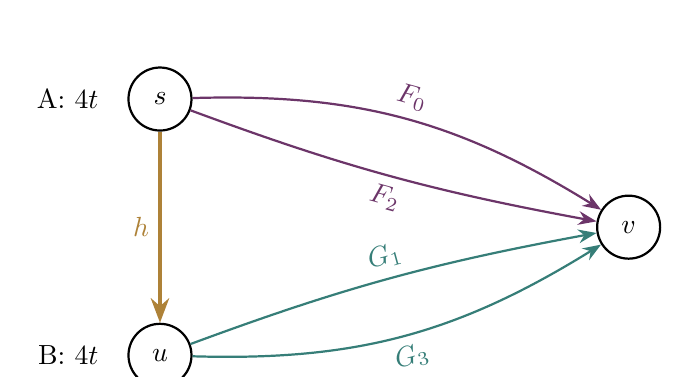
\begin{tikzpicture}[>=Stealth,thick,scale=0.93]
\node[circle,draw,minimum size=8mm] (s) at (0,2.2) {$s$};
\node[circle,draw,minimum size=8mm] (u) at (0,-1.3) {$u$};
\node[circle,draw,minimum size=8mm] (v) at (6.4,0.45) {$v$};
\draw[->,plum] (s) to[bend left=17] node[above,sloped] {$F_0$} (v);
\draw[->,plum] (s) to[bend right=5] node[below,sloped] {$F_2$} (v);
\draw[->,teal] (u) to[bend left=5] node[above,sloped] {$G_1$} (v);
\draw[->,teal] (u) to[bend right=17] node[below,sloped] {$G_3$} (v);
\draw[->,ochre,line width=1.3pt] (s) -- node[left] {$h$} (u);
\node[anchor=east,align=right] at (-0.7,2.2) {A: $4t$};
\node[anchor=east,align=right] at (-0.7,-1.3) {B: $4t$};
\end{tikzpicture}
\caption{The five-link example. Commodity A can use either direct edge, or the connector followed by either shared edge. Commodity B chooses between the shared edges. Every directed path is a route. Near $t=1$ the connector starts to carry flow at $t=1$.}
\label{fig:network}
\end{figure}

Every edge has the conventional BPR form $a_e[1+0.15(z/C_e)^4]$ with $C_e=(0.15a_e/b_e)^{1/4}$. The table shows that at $t=1$ the volume-to-capacity ratios lie between $0.96$ and $1.35$ and congested times are $1.13$ to $1.5$ times free-flow times. These are ordinary peak-period values, so the example does not depend on extreme capacities.

Let $F(T)$ and $G(T)$ be the bank delays at total bank load $T$. At $T=4$,
\begin{equation}\label{eq:quinticjets}
 F(4)=3,\quad G(4)=2,\quad F'(4)=G'(4)=\tfrac25,\quad
 F''(4)=G''(4)=\tfrac{42}{125},\quad F'''(4)-G'''(4)=\tfrac{63}{1250}.
\end{equation}
The two bank delay curves agree to second order. The connector route is cheaper when $\Delta(t)=F(4t)-G(4t)-1>0$, and $\Delta(t)=\tfrac{336}{625}\delta^3+O(\delta^4)$. For $t>1$ the connector flow solves $F(4t-x)=G(4t+x)+1+x^4$. Theorem~\ref{thm:main} below, with $m=3$ and $p=4$, gives
\begin{align}
 x(t)&=\tfrac{84}{125}\delta_+^3+O(\delta_+^4),\label{eq:fivex}\\
 E(t)&=E_0(t)-\tfrac{84672}{78125}\delta_+^5+O(\delta_+^6),\qquad E_0(t)=4t\bigl(F(4t)+G(4t)\bigr).\label{eq:fiveE}
\end{align}
Here $O(\delta_+^r)$ vanishes on the left and has derivative-controlled remainders on the right (Lemma~\ref{lem:remainder}), so these expansions are statements about derivatives, not only about values. In particular $E(1)=20$ and $E'(1^-)=E'(1^+)=164/5$. The first four derivatives of $E$ and $P$ are continuous at $t=1$, and their fifth derivatives jump: $E^{(5)}$ by $-2032128/15625\approx-130.06$ and $P^{(5)}$ by about $-6.581$. Just below $t=1$ the only cheapest routes of A are the two direct edges. Just above it the two connector routes are cheapest too. The set of cheapest routes itself expands; this is not an artefact of a choice of route decomposition. \status{proof; exact; the $P^{(5)}$ value uses $S(1)=19.762875963175$, computed numerically and agreeing with direct optimisation}

The same construction with $p=2$ has congestion coefficients $(1,1/27,1/18,1/4,1)$ in table order and the same free-flow costs. There every cost has positive second derivative on $[0,\infty)$, and again $E,P\in C^4\setminus C^5$.

\emph{A contraction.} Exchanging the two banks' edge sets gives a five-link contraction: direct edges $5/2+z^4/162$ and $11/4+z^4/4$, shared edges $1+z^4$ and $5/3+z^4/243$, connector $1+z^4$, demands $4t$. Now $\Delta(t)=-\tfrac{336}{625}\delta^3+O(\delta^4)$. The connector is used just below $t=1$ with every bank edge loaded, and it is not cheapest above $t=1$. Exact series give $E-E_0=-\tfrac{84672}{78125}\delta^5+O(\delta^6)$ on the active side $\delta<0$, so $E,P\in C^4\setminus C^5$ with equal slopes $164/5$. \status{proof via Proposition~\ref{prop:localcontact}; exact}

\subsection{Any finite order}\label{sec:family}

Fix $p>1$ and an odd integer $m\ge3$, and set
\begin{equation}\label{eq:parameters}
 N=2^{m-1},\qquad w_j=\binom mj,\qquad u_j=j+1\quad(0\le j\le m).
\end{equation}
The graph has vertices $s,u,v$. For each even $j$ the direct bank $F$ has an edge $s\to v$, and for each odd $j$ the shared bank $G$ has an edge $u\to v$. A connector runs from $s$ to $u$. The costs are
\begin{align}
 c_j^F(z)&=3-\frac1{u_j}+\frac{z^p}{u_jw_j^p}\quad(j\text{ even}),\qquad
 c_j^G(z)=2-\frac1{u_j}+\frac{z^p}{u_jw_j^p}\quad(j\text{ odd}),\label{eq:FGcost}\\
 h(z)&=1+z^p.\label{eq:hcost}
\end{align}
Commodity A travels from $s$ to $v$ and commodity B from $u$ to $v$, each with demand $Nt$, and every directed path is a route. The graph has $m+2$ edges, all of the form $a_e+b_ez^p$ with $a_e,b_e>0$. For $m=3$, $p=4$ this is the five-link example. Put
\begin{equation}\label{eq:constants}
 \Pi_{m,p}=\prod_{k=0}^{m-1}(1-kp),\qquad
 a=\frac{4p\Pi_{m,p}}{(m+2)^{m+1}},\qquad
 k_x=\frac{N\Pi_{m,p}}{(m+2)^m},\qquad k_E=m\,a\,k_x.
\end{equation}
All are positive, because $m-1$ of the factors of $\Pi_{m,p}$ are negative and $m-1$ is even.

\begin{theorem}[Common-power transitions of arbitrary order]\label{thm:main}
For the network \eqref{eq:FGcost}--\eqref{eq:hcost}:
\begin{enumerate}[label=(\roman*),nosep]
\item The regime strictly expands at $t=1$. Every bank edge has load $w_j>0$ there and the connector has load zero. The connector routes are not cheapest just below $1$, and every edge is loaded for every $t>1$.
\item The connector flow $x$ is $C^{m-1}$ but not $C^m$ at $1$. Its first nonzero term on the right is $k_x\delta^m$, and its $m$-th derivative jumps by $m!\,k_x$.
\item The optimal cost $S$ is positive and real analytic near $1$. There is a real-analytic $E_0$ with $E=E_0$ just below $1$, and the first nonzero term of $E-E_0$ on the right is $-k_E\delta^{2m-1}$.
\item $E$ and $P$ belong to $C^{2m-2}\setminus C^{2m-1}$ at $1$, with
\begin{equation}\label{eq:Ejump}
\begin{gathered}
 E^{(2m-1)}(1^+)-E^{(2m-1)}(1^-)=-(2m-1)!\,k_E,\\
 P^{(2m-1)}(1^+)-P^{(2m-1)}(1^-)=-\frac{(2m-1)!\,k_E}{S(1)}.
\end{gathered}
\end{equation}
In particular both first derivatives are continuous across the expansion.
\end{enumerate}
These conclusions hold for every real $p>1$. For integer $p$ the remainders in (ii) and (iii) are analytic multiples of $\delta^{m+1}$ and $\delta^{2m}$. For noninteger $p$ they are controlled by Lemma~\ref{lem:remainder}.
\end{theorem}

With $p=4$ fixed, the order of smoothness grows without bound across this family of finite networks. Positive cost coefficients therefore impose no fixed limit on how many derivatives can agree at an expansion. The affine case is different: there CDS Theorem~4.4(ii) gives strictness, and the construction degenerates at $p=1$.

\subsubsection*{Proof of Theorem~\ref{thm:main}}

\emph{Inverse bank curves.} Put $\alpha_p=1/p\in(0,1)$. At total bank load $N$, branch $j$ has load $w_j$, and the bank delays are $3$ and $2$. When the delay of bank $F$ is $3+s$ and that of bank $G$ is $2+s$, the total loads are
\begin{equation}\label{eq:supply}
 q_F(s)=\sum_{j\text{ even}}w_j(1+u_js)^{\alpha_p},\qquad q_G(s)=\sum_{j\text{ odd}}w_j(1+u_js)^{\alpha_p},
\end{equation}
for $s>-1/(m+1)$, where all branches are loaded. These curves are analytic and strictly increasing, and their inverses define $F$ and $G$ near $N$ and on $[N,\infty)$. The binomial identities
\begin{equation}\label{eq:moments}
 \sum_{j=0}^m(-1)^j\binom mj(j+1)^k=0\quad(0\le k<m),\qquad \sum_{j=0}^m(-1)^j\binom mj(j+1)^m=-m!
\end{equation}
follow by applying an $m$-th finite difference to polynomials of degree $k$; the sign of the last uses odd $m$. With
\begin{equation}\label{eq:cA}
 c_m=\alpha_p(\alpha_p-1)\cdots(\alpha_p-m+1)>0,\qquad \beta=q_F'(0)=q_G'(0)=\frac{N(m+2)}{2p},
\end{equation}
Taylor expansion of \eqref{eq:supply} gives $q_F(s)-q_G(s)=-c_ms^m+O(s^{m+1})$. The sign holds for all $s>0$. With $\varphi(r)=r^{\alpha_p}$, repeated use of the fundamental theorem of calculus gives
\begin{equation}\label{eq:integraldifference}
 q_F(s)-q_G(s)=-s^m\int_{[0,1]^m}\varphi^{(m)}\Bigl(1+s\bigl(1+\textstyle\sum_{i=1}^m\theta_i\bigr)\Bigr)\dd\theta,
\end{equation}
and $\varphi^{(m)}(r)=c_mr^{\alpha_p-m}>0$, so the difference is negative for $s>0$ and positive for small $s<0$.

\emph{The route gap.} Put $\widehat\Delta(T)=F(T)-G(T)-1$. Analytic inversion gives $\widehat\Delta(T)=c_m\beta^{-m-1}(T-N)^m+O((T-N)^{m+1})$. To check the coefficient, set $s=G(T)-2$. Then $q_G(s)=T$ and $q_F(s)=T-c_ms^m+O(s^{m+1})$, so the increment of $s$ needed to make $q_F$ equal $T$ is $(c_m/\beta)s^m+O(s^{m+1})$, while $s=(T-N)/\beta+O((T-N)^2)$. For every $T>N$, \eqref{eq:integraldifference} gives $q_F(G(T)-2)<T$, hence
\begin{equation}\label{eq:globalH}
 \widehat\Delta(T)>0\quad(T>N),
\end{equation}
while $\widehat\Delta(T)<0$ for $T<N$ close to $N$. The route gap of the connector route without connector flow is therefore
\begin{equation}\label{eq:D}
 \Delta(t)=F(Nt)-G(Nt)-1=a\delta^m+O(\delta^{m+1}),\qquad a=\frac{c_mN^m}{\beta^{m+1}},
\end{equation}
and $c_m=\Pi_{m,p}/p^m$ with $N=2^{m-1}$ gives the constant in \eqref{eq:constants}.

\emph{The equilibrium and its regime.} If $x$ units of A use the connector, bank $F$ carries $Nt-x$ and bank $G$ carries $Nt+x$, and each bank splits its load so as to equalise the delays of its used edges. The connector flow is positive exactly when
\begin{equation}\label{eq:scalar}
 F(Nt-x)-G(Nt+x)-1-x^p=0
\end{equation}
has a positive root. The left side strictly decreases in $x$. For $t<1$ near $1$ it is negative at $x=0$, so the connector is unused and its routes are strictly more expensive. For $t>1$ it is positive at $x=0$ by \eqref{eq:globalH}, and at $x=N(t-1)$ it equals $3-G(N(2t-1))-1-[N(t-1)]^p<0$. Hence there is a unique root with
\begin{equation}\label{eq:rootbound}
 0<x(t)<N(t-1)\qquad(t>1).
\end{equation}
Both bank totals exceed $N$, so every bank edge is loaded, and so is the connector. All costs in \eqref{eq:scalar} are analytic at this root, with negative $x$-derivative, so the equilibrium loads are analytic for $t>1$. These loads come from route flows: in bank $G$ split both the $x$ units of A and the $Nt$ units of B across the branches in the common load proportions. Then every route used is cheapest, and \eqref{eq:scalar} makes the direct and connector routes of A equally cheap. Just below $1$ the connector routes are strictly more expensive. The complete regime therefore strictly expands at $t=1$, whatever route decomposition is chosen. This proves (i).

\emph{The onset.} For integer $p$, the analytic implicit function theorem applied to \eqref{eq:scalar} at $(t,x)=(1,0)$ gives a signed analytic branch with $x$-derivative $-2/\beta$, and on the right
\begin{equation}\label{eq:xasymptotic}
 x(t)=k_x\delta^m+O(\delta^{m+1}),\qquad k_x=\frac{\beta a}2.
\end{equation}
The flow is zero on the left. For noninteger $p$ there is no analytic extension of $x^p$ across zero, and we argue as follows. Analyticity of the bank curves gives analytic $d,\ell_1,\rho$ with
\begin{equation}\label{eq:implicitgeneral}
 F(Nt-x)-G(Nt+x)-1=\delta^md(\delta)-\ell_1(\delta)x+x^2\rho(\delta,x),\qquad d(0)=a,\ \ell_1(0)=2/\beta.
\end{equation}
For $\delta>0$ put $x=\delta^mU$ and $y=\delta^{m(p-1)}$. Dividing by $\delta^m$ gives
\begin{equation}\label{eq:Uequation}
 d(\delta)-\ell_1(\delta)U+\delta^mU^2\rho(\delta,\delta^mU)-yU^p=0,
\end{equation}
which is analytic in $(\delta,y,U)$ near $(0,0,k_x)$, since $k_x>0$, with $U$-derivative $-2/\beta$ there. Hence there is an analytic $U(\delta,y)$ with $U(0,0)=k_x$ and
\begin{equation}\label{eq:twovar}
 x(t)=\delta^mU(\delta,\delta^{m(p-1)})\qquad(\delta>0).
\end{equation}

\begin{lemma}[Differentiating the remainder]\label{lem:remainder}
Let $U(\delta,y)=\sum_{i,j\ge0}u_{ij}\delta^iy^j$ converge absolutely for $|\delta|,|y|\le\rho_0$, with $0<\rho_0\le1$. Let $\beta_0>0$, let $q\ge1$ be an integer, and put $\varrho=\min(1,\beta_0)$. For $0<\delta\le\delta_1:=\min\bigl(\rho_0/2,(\rho_0/2)^{1/\beta_0}\bigr)$ define $R_q(\delta)=\delta^q[U(\delta,\delta^{\beta_0})-U(0,0)]$. Then for $0\le r\le q$,
\[
 |R_q^{(r)}(\delta)|\le C_r\,\delta^{q-r+\varrho},\qquad
 C_r=\delta_1^{-\varrho}\sum_{(i,j)\ne(0,0)}|u_{ij}|\,(q+i+\beta_0j)^r\,(\rho_0/2)^{i+j}<\infty.
\]
Consequently the function equal to $0$ for $\delta\le0$ and to $\delta^qU(\delta,\delta^{\beta_0})$ for $\delta>0$ is $C^{q-1}$ near $0$, and its $q$-th derivative jumps by $q!\,U(0,0)$ at $0$.
\end{lemma}
\begin{proof}
For $0<\delta\le\delta_1$ we have $\delta\le\rho_0/2$ and $\delta^{\beta_0}\le\rho_0/2$. Each term $u_{ij}\delta^{q+i+\beta_0j}$ with $(i,j)\ne(0,0)$ has $r$-th derivative of absolute value at most $|u_{ij}|(q+i+\beta_0j)^r\delta^{q+i+\beta_0j-r}$. Since $i+\beta_0j\ge\varrho$, and the exponent $i+\beta_0j-\varrho$ is nonnegative, $\delta^{i+\beta_0j}=\delta^\varrho\delta^{i+\beta_0j-\varrho}\le\delta^\varrho\delta_1^{i+\beta_0j-\varrho}\le\delta^\varrho\delta_1^{-\varrho}(\rho_0/2)^{i+j}$. The constant $C_r$ is finite because $(q+i+\beta_0j)^r2^{-(i+j)}$ is bounded and $\sum|u_{ij}|\rho_0^{i+j}<\infty$. The differentiated series therefore converges uniformly on $(0,\delta_1]$, which justifies termwise differentiation and gives the bound. Since every $R_q^{(r)}$ with $r\le q$ tends to $0$ as $\delta\downarrow0$, the extension of $R_q$ by zero is $C^q$ with vanishing derivatives at $0$. Adding $U(0,0)\delta_+^q$, which is $C^{q-1}$ with $q$-th derivative jump $q!$, gives the last assertion.
\end{proof}

Applying Lemma~\ref{lem:remainder} to \eqref{eq:twovar} with $q=m$ and $\beta_0=m(p-1)$ proves (ii) for every real $p>1$.

\emph{Why total cost hides more derivatives.} Every user of A pays $F(Nt-x)$ and every user of B pays $G(Nt+x)$, because the connector route costs the same as the direct route. Hence
\begin{equation}\label{eq:Ephysical}
 E(t)=Nt\bigl[F(Nt-x(t))+G(Nt+x(t))\bigr],\qquad E_0(t)=Nt\bigl[F(Nt)+G(Nt)\bigr],
\end{equation}
where $E_0$ is analytic near $1$ and equals $E$ on the left. Taylor expansion in $x$ gives
\begin{equation}\label{eq:Ecancel}
 E-E_0=Nt\bigl[G'(Nt)-F'(Nt)\bigr]x+O(x^2)=-t\Delta'(t)x+O(x^2).
\end{equation}
Since $\Delta'$ has order $m-1$ and $x$ has order $m$, the first term is $-ma\,k_x\delta^{2m-1}=-k_E\delta^{2m-1}$, and the quadratic term starts at order $2m$. For real $p>1$, \eqref{eq:twovar} gives $E-E_0=\delta^{2m-1}V_E(\delta,\delta^{m(p-1)})$ for $\delta>0$, with $V_E$ analytic and $V_E(0,0)=-k_E$. Lemma~\ref{lem:remainder} with $q=2m-1$ gives \eqref{eq:Ejump} for $E$. Also
\begin{equation}\label{eq:allfirst}
 E(1)=5N,\qquad E'(1)=5N+\frac{2N^2}{\beta}=N\Bigl(5+\frac{4p}{m+2}\Bigr).
\end{equation}

\emph{The optimum.} The common-power scaling of O'Hare et al.\ \cite[Theorem~3.5]{OCW2016} handles $S$. Put $\gamma=(p+1)^{1/p}>1$. The marginal social cost of edge $e$ is $a_e+(p+1)b_ez^p=c_e(\gamma z)$. Scaling a feasible flow by $\gamma$ scales every demand by $\gamma$, so the optimality conditions give
\begin{equation}\label{eq:optflow}
 z_e^\opt(t)=\gamma^{-1}z_e^\eq(\gamma t),
\end{equation}
and the optimal loads are unique by strict convexity. By \eqref{eq:rootbound} every equilibrium load at $\gamma t$ is positive and analytic for $t$ near $1$, so
\begin{equation}\label{eq:optcost}
 S(t)=\frac1\gamma\sum_e\Bigl[a_ez_e^\eq(\gamma t)+\frac{b_e}{p+1}\bigl(z_e^\eq(\gamma t)\bigr)^{p+1}\Bigr]=\frac{V(\gamma t)}{\gamma}
\end{equation}
is positive and analytic there, where $V$ is the Beckmann value. (In general $S(t)\ne E(\gamma t)/\gamma$, because the congestion terms carry different factors.) Dividing by $S$, the quotient $P_0=E_0/S$ is analytic, and the leading term of $P-P_0$ is $-k_E\delta^{2m-1}/S(1)$. Lemma~\ref{lem:remainder} gives the jump of $P$ in \eqref{eq:Ejump}. \qed

\begin{remark}[Potential interpretation]\label{rem:potential}
After the bank splits are optimised, the Beckmann objective as a function of the connector flow is $B(t,x)=\int_0^{Nt-x}F+\int_0^{Nt+x}G+\int_0^xh$. Its minimum over $x\ge0$ differs from $B(t,0)$ by $-\Delta(t)_+^2/(2L_0)$ to leading order, with $L_0=F'+G'+h'(0)$, so by order $2m$. Since $E=tV'$ (Proposition~\ref{prop:Sregular}), differentiation explains the order $2m-1$ of $E-E_0$. The same mechanism gives the optimum-side transition of Section~\ref{sec:optimumside}.
\end{remark}

\section{How few links are needed}\label{sec:minimal}

How small can a network be and still hide a regime change in this way? The answer depends on the cost class and on the type of breakpoint. Table~\ref{tab:minimaledges} collects what is proved. Throughout, demands are proportional with every $r_k>0$, every simple path is a route, and ``equal slopes'' means $E'(t_0^-)=E'(t_0^+)$ at a nested breakpoint $t_0>0$.

\begin{theorem}[Minimal link counts]\label{thm:minimal}
Consider networks with costs $a_e+b_ez^p$, $a_e,b_e>0$, and one common real exponent $p>1$. Every network with at most four edges has strict slope jumps of $E$ and of $P$ at every nested breakpoint, in the direction of Theorem~\ref{thm:weakcomparison}. Hence five is the minimum number of edges permitting equal slopes, both at nested expansions and at nested contractions.
\end{theorem}

The lower bound is Theorem~\ref{thm:fouredge}, proved in Appendix~\ref{app:minimality}. The five-link expansion and contraction of Section~\ref{sec:fiveedge} attain it. The proof is a finite case analysis with an explicit inequality closing each case (Table~\ref{tab:minimality}). Its outline is as follows.
\begin{itemize}[nosep]
\item By Lemma~\ref{lem:tangencycomparison}, equal slopes force a tangency of the gap of a new route.
\item If the smaller regime has no demand-preserving load changes ($\Kc_{R_s}=\{0\}$), the common-power identity $Dq=p(c_0-a)/t_0$ makes the gap a function $\alpha+\beta t^p$, which cannot be tangent to zero without vanishing identically. This disposes of every connected graph with at least four vertices or at most three edges.
\item Networks whose cycles are all parallel banks have no contractions, and their expansions are strict because a joining branch lowers the derivative of the bank delay to zero.
\item The remaining graph is a transitive triangle with one side doubled. There, a curvature inequality for parallel banks, $\ell''-(p-1)\ell'/t>0$ unless all free-flow costs in the bank are equal, rules out every tangency.
\end{itemize}

\begin{table}[htbp]
\centering\small
\begin{tabularx}{\linewidth}{@{}>{\raggedright\arraybackslash}p{4.3cm}>{\raggedright\arraybackslash}p{2.3cm}>{\raggedright\arraybackslash}p{2.6cm}X@{}}
\toprule
Cost class & Breakpoint & Minimum edges & Evidence\\
\midrule
Strictly convex polynomials & expansion & $3$ & Example~\ref{ex:cubic}; two edges never suffice (Remark~\ref{rem:twoedges})\\
BPR, edge-specific exponents & contraction & $3$ & Example~\ref{ex:hetero}; Remark~\ref{rem:twoedges}\\
BPR, edge-specific exponents & expansion & $4$ or $5$ (open) & three edges excluded (Proposition~\ref{prop:hetero}, Remark~\ref{rem:hetero}); five-link example\\
BPR, common exponent & expansion & $5$ & Theorems~\ref{thm:main} and~\ref{thm:fouredge}\\
BPR, common exponent & contraction & $5$ & bank-swapped example; Theorem~\ref{thm:fouredge}\\
\bottomrule
\end{tabularx}
\caption{Minimum numbers of edges for equal one-sided slopes at nested breakpoints. Positive free-flow and congestion coefficients throughout.}
\label{tab:minimaledges}
\end{table}

\begin{remark}[Two edges never suffice]\label{rem:twoedges}
Let every cost be $C^1$ with $c_e'(z)>0$ for $z>0$. If a network with at most two edges has a breakpoint, some commodity has two routes, so the two edges are parallel, say $s\to v$, and carry a total demand $Qt$ with $Q>0$. Their common delay $\ell(Qt)$ is strictly increasing in $t$, so an edge can only join: there are no contractions. Suppose edge $2$ joins at $t_0$, so $c_2(0)=\ell(Qt_0)$. To the left only edge $1$ is used, with positive load, and $\ell'(Qt_0^-)=c_1'(Qt_0)>0$. To the right the loads satisfy $c_1(y_1)=c_2(y_2)$ with $y_1+y_2=Qt$. Hence $y_2/(Qt-Qt_0)\to c_1'/(c_1'+c_2'(0))$, which is read as $1$ if $c_2'(0)=0$, and $\ell'(Qt_0^+)=c_1'c_2'(0)/(c_1'+c_2'(0))<c_1'$. Since $E=Qt\,\ell(Qt)$, the slope of $E$ drops strictly, by $Q^2t_0[\ell'(Qt_0^-)-\ell'(Qt_0^+)]>0$.
\end{remark}

These minima concern the stated classes only. In the two-bank architecture a sharper, order-dependent count holds: contacts of orders $m_1,\dots,m_\ell$ need exactly $2+\sum_jm_j$ edges (Appendix~\ref{app:contacts}). That count is specific to the architecture and is not a lower bound for arbitrary graphs.

\section{How robust is a hidden transition?}\label{sec:robustness}

The examples impose exact equalities on the bank delay curves. This section asks what survives when they are perturbed, and shows that the price of anarchy has a second, optimum-side transition. All statements refer to the family of Theorem~\ref{thm:main}, with route gap $\Delta(t)=a\delta^m+O(\delta^{m+1})$ and $\beta=q_F'(0)$.

\subsection{A small change of free-flow cost restores the kink}

\begin{proposition}[Perturbation law]\label{prop:perturbation}
Change only the connector cost, to $h_\varepsilon(x)=1+\varepsilon+x^p$. For every sufficiently small $\varepsilon\ne0$ the nearby expansion occurs at a unique $t_\varepsilon$ with
\begin{equation}\label{eq:thresholdperturbation}
 t_\varepsilon-1=\sgn(\varepsilon)(|\varepsilon|/a)^{1/m}+O(|\varepsilon|^{2/m}).
\end{equation}
Its slope jump is strictly positive:
\begin{equation}\label{eq:exactperturbation}
 J_E(\varepsilon):=E_\varepsilon'(t_\varepsilon^-)-E_\varepsilon'(t_\varepsilon^+)=\frac{t_\varepsilon[\Delta'(t_\varepsilon)]^2}{F'(Nt_\varepsilon)+G'(Nt_\varepsilon)}\sim\frac\beta2m^2a^{2/m}|\varepsilon|^{2-2/m}.
\end{equation}
The jump of $P$ is $J_E(\varepsilon)/S_\varepsilon(t_\varepsilon)$, and $S_\varepsilon(t_\varepsilon)\to S(1)>0$.
\end{proposition}
\begin{proof}
The inactive route gap becomes $\Delta(t)-\varepsilon$. By \eqref{eq:D} and its differentiated expansion, $\Delta$ is strictly increasing near $1$ with a single critical point at $1$, which gives \eqref{eq:thresholdperturbation}. At the shifted transition the connector flow has right derivative $\Delta'(t_\varepsilon)/(F'(Nt_\varepsilon)+G'(Nt_\varepsilon))$, because $h_\varepsilon'(0)=0$, and left derivative zero. Differentiating \eqref{eq:Ephysical} gives the exact formula. Substituting \eqref{eq:thresholdperturbation}, $\Delta'(t)\sim ma(t-1)^{m-1}$ and $F'(N)+G'(N)=2/\beta$ gives the asymptotic one. All bank loads near $t_\varepsilon$ stay positive. The all-positive marginal-cost equilibrium near $\gamma$ persists for small $\varepsilon$, so $S_\varepsilon$ is smooth near $t_\varepsilon$, and the quotient rule applies.
\end{proof}

In the five-link example the threshold moves on the scale $|\varepsilon|^{1/3}$, but the kink grows only like $|\varepsilon|^{4/3}$. Small perturbations therefore restore a kink that is much smaller than the perturbation (Section~\ref{sec:practice} gives numbers).

\subsection{A small change of the demand ratio}

Keep the network fixed and replace the demand ray by $(N(1+\eta)t,Nt)$. With $b_0=N/\beta$ the inactive gap is $\Delta_\eta(1+\delta)=a\delta^m+b_0\eta+O(\delta^{m+1}+|\eta\delta|+\eta^2)$.

\begin{proposition}[Demand-ratio unfolding]\label{prop:demandunfolding}
For every sufficiently small $\eta\ne0$ there is a unique nearby transition. It is an expansion, with
\[
 t_\eta-1=-\sgn(\eta)\Bigl(\frac{b_0|\eta|}{a}\Bigr)^{1/m}+O(|\eta|^{2/m}),\qquad
 E_\eta'(t_\eta^-)-E_\eta'(t_\eta^+)\sim\frac\beta2m^2a^{2/m}b_0^{2-2/m}|\eta|^{2-2/m}.
\]
The jump of $P$ is the jump of $E$ divided by $S_\eta(t_\eta)\to S(1)>0$.
\end{proposition}
\begin{proof}
Put $\epsilon_0=|\eta|^{1/m}$ and $\delta=\epsilon_0y$. Dividing the gap by $\epsilon_0^m$ gives $ay^m+\sgn(\eta)b_0+\epsilon_0\varrho(y,\epsilon_0)$ with $\varrho$ analytic. The limiting polynomial has one real root, which is simple, and the implicit function theorem continues it. Any nearby zero has $|\delta|$ bounded above and below by multiples of $\epsilon_0$, because the first two terms dominate, so compactness in $y$ gives uniqueness. At the root $\Delta_\eta'(t_\eta)\sim ma^{1/m}b_0^{(m-1)/m}|\eta|^{(m-1)/m}>0$. Proposition~\ref{prop:localcontact}, with contact order one and curvature tending to $2/\beta$, gives the jump. The all-positive equilibrium near the multiplier $\gamma$ persists under small changes of the demand ratio, so the optimum remains analytic near $t_\eta$.
\end{proof}

For $m=3$, $p=4$ we have $b_0=8/5$, the threshold shifts by $(125|\eta|/42)^{1/3}$ to leading order, and the slope jump is $C_\eta|\eta|^{4/3}$ with $C_\eta^3=5267275776/1953125$, so $C_\eta\approx13.919$.

\subsection{Transverse demand directions}

Now vary the two demands $(q_A,q_B)$ independently near $(N,N)$, with the costs fixed. Let $E_0(q_A,q_B)=q_AF(q_A)+q_BG(q_B)$, and put
\[
 f_1=F'(N)=G'(N)=1/\beta,\qquad f_2=F''(N)=G''(N)>0,\qquad \chi=f_1/2+Nf_2/4>0.
\]
These equalities hold in the family because $m\ge3$, and $f_2>0$ because the bank throughput curves are strictly concave.

\begin{proposition}[Anisotropy at the high-contact demand]\label{prop:anisotropy}
For $u_A=q_A-N$, $u_B=q_B-N$ and $\rho=(u_A^2+u_B^2)^{1/2}$,
\begin{equation}\label{eq:planarexpansion}
 E(q_A,q_B)-E_0(q_A,q_B)=-\chi(u_A-u_B)_+^2+o(\rho^2).
\end{equation}
So $E$ is Fr\'echet differentiable at $(N,N)$, with gradient $(3+N/\beta,\,2+N/\beta)$, but has no second-order Taylor expansion there. Along every straight demand path $q_A=N+v_0\delta$, $q_B=N+w_0\delta$ with $v_0\ne w_0$, both $E$ and $P$ are $C^1$ but not $C^2$. Their second-derivative jumps, active minus inactive side, are $-2\chi(v_0-w_0)^2$ and that quantity divided by $S(N,N)$.
\end{proposition}
\begin{proof}
The inactive gap is $f_1(u_A-u_B)+O(\rho^2)$. The connector residual has $x$-derivative $-2f_1$ at the base point, and the cost $x^p$ contributes $O(\rho^p)$. So the implicit function theorem gives the positive root $x=(u_A-u_B)_+/2+O(\rho^2+\rho^p)$. At an active equilibrium
\[
 E-E_0=-\{q_AF'(q_A)-q_BG'(q_B)\}x+\tfrac12\{q_AF''(q_A)+q_BG''(q_B)\}x^2+O(x^3).
\]
The two braces equal $(f_1+Nf_2)(u_A-u_B)+O(\rho^2)$ and $2Nf_2+O(\rho)$. Substitution gives \eqref{eq:planarexpansion}. The positive part of a quadratic is not a quadratic form, which proves the statements about Fr\'echet differentiability. On a straight path put $\sigma=\sgn(v_0-w_0)$ and $\tau=\sigma\delta>0$ on the active side. Then $x=\tau U(\tau,\tau^{p-1})$ and $E-E_0=\tau^2V(\tau,\tau^{p-1})$ with $U,V$ analytic and $V(0,0)=-\chi(v_0-w_0)^2$. Lemma~\ref{lem:remainder} gives the claims for $E$. The common-power scaling maps a neighbourhood of $(N,N)$ to a neighbourhood of $\gamma(N,N)$, where every equilibrium edge is loaded, so the optimum is jointly analytic there, which gives the claims for $P$.
\end{proof}

For the binomial family,
\[
 \chi=\frac{p\{2(m+2)^2+(p-1)(m+1)(m+4)\}}{2N(m+2)^3}.
\]
In the five-link example $\chi=67/125$ and $\nabla E(4,4)=(23/5,18/5)$. The high smoothness therefore belongs to the proportional ray, not to the demand point. Along every other straight path through the same demand vector the second derivative jumps. The expansion \eqref{eq:planarexpansion} is pointwise and does not say that $E$ is $C^1$ on a whole neighbourhood: nearby points of the boundary can have first-derivative jumps.

\subsection{The optimum changes its routes first}\label{sec:optimumside}

By \eqref{eq:optflow} the optimum at $t$ uses the equilibrium loads at $\gamma t$, scaled by $1/\gamma$. Its connector therefore activates at $t=1/\gamma$, before the equilibrium connector does. In the five-link example $1/\gamma=5^{-1/4}\approx0.669$, and at $t=1$ the optimum already sends $0.00643$ units over the connector.

\begin{theorem}[Optimum-side transition]\label{thm:optimumtransition}
In the family of Theorem~\ref{thm:main}, let $V$ be the Beckmann value along the equilibrium ray and $V_0$ its analytic continuation without the connector. Then
\begin{equation}\label{eq:Vexpansion}
 V(T)-V_0(T)=-\frac{k_E}{2m}(T-1)_+^{2m}+\text{(derivative-controlled higher order)},
\end{equation}
and $S(t)=V(\gamma t)/\gamma$. Hence $S\in C^{2m-1}\setminus C^{2m}$ at $t=1/\gamma$, with
\[
 S^{(2m)}(1/\gamma^+)-S^{(2m)}(1/\gamma^-)=-(2m-1)!\,k_E\,\gamma^{2m-1}.
\]
If $E$ is $C^{2m}$ near $1/\gamma$, then $P\in C^{2m-1}\setminus C^{2m}$ at $1/\gamma$, with
\begin{equation}\label{eq:Poptjump}
 P^{(2m)}(1/\gamma^+)-P^{(2m)}(1/\gamma^-)=\frac{(2m-1)!\,k_E\,\gamma^{2m-1}E(1/\gamma)}{S(1/\gamma)^2}>0.
\end{equation}
In the five-link example $E$ is analytic near $1/\gamma$, so $S,P\in C^5\setminus C^6$ there and the jump \eqref{eq:Poptjump} is $\approx+89.68$.
\end{theorem}
\begin{proof}
Proposition~\ref{prop:Sregular} gives $V'(T)=E(T)/T$ along the ray, and the restricted problem without the connector gives $V_0'=E_0/T$ with $V_0$ analytic near $1$. Since $V=V_0$ for $T\le1$ near $1$,
\[
 V(T)-V_0(T)=\int_1^T\frac{E(\tau)-E_0(\tau)}{\tau}\dd\tau .
\]
By the proof of Theorem~\ref{thm:main}, $E-E_0=\delta^{2m-1}V_E(\delta,\delta^{m(p-1)})$ on the right. Dividing by $\tau=1+\delta$ and integrating the absolutely convergent series term by term gives $\delta^{2m}\widetilde V(\delta,\delta^{m(p-1)})$ with $\widetilde V$ analytic and $\widetilde V(0,0)=-k_E/(2m)$. This is \eqref{eq:Vexpansion}, and Lemma~\ref{lem:remainder} applies. The formula $S(t)=V(\gamma t)/\gamma$ is \eqref{eq:optcost}. Substituting $T=\gamma t$ gives $S-S_0=-\frac{k_E\gamma^{2m-1}}{2m}(t-1/\gamma)_+^{2m}+\cdots$, which yields the jump of $S^{(2m)}$. If $E$ is $C^{2m}$, the highest-order jump of $P=E/S$ comes only from $1/S$, and $(1/S)^{(2m)}$ jumps by $-S^{(2m)}\text{-jump}/S^2$. For the five-link example, exact interval arithmetic shows that on $[1/\gamma-1/100,1)$ the equilibrium connector is strictly unused and all four bank edges are loaded, so $E$ is analytic near $1/\gamma$. The numerical value uses $E(1/\gamma)\approx11.920$, $S(1/\gamma)=17/5^{1/4}\approx11.369$ and $P(1/\gamma)\approx1.0485$. \status{proof; exact interval check; numerical constants}
\end{proof}

So a planner who watches the price of anarchy sees two hidden transitions as demand grows: the optimum's at $1/\gamma$, with five continuous derivatives in the quartic example, and the equilibrium's at $1$, with four. In CDS Example~4.3 the optimum also changes regime at a point where $S$ stays smooth. Theorem~\ref{thm:optimumtransition} adds the exact order of that smoothness for the present family.

\section{What this means for assignment practice}\label{sec:practice}

This section translates the results into the terms of a modeller who runs assignments at increasing demand and watches total travel time or the price of anarchy. Unless stated otherwise, the numbers are high-precision numerical computations (50--60 significant digits) for the five-link example, made with the physical costs. They agree with the exact series.

\subsection{Hidden activation below assignment tolerance}

Table~\ref{tab:hidden} shows how little the new route is used after the expansion at $t=1$.

\begin{table}[htbp]
\centering\small
\begin{tabular}{rrrr}
\toprule
$\delta=t-1$ & connector flow $x$ & $x$ as \% of A's demand & $(E-E_0)/E_0$\\
\midrule
$0.01$ & $6.33\times10^{-7}$ & $1.6\times10^{-5}$ & $-4.9\times10^{-12}$\\
$0.05$ & $6.31\times10^{-5}$ & $1.5\times10^{-3}$ & $-1.0\times10^{-8}$\\
$0.10$ & $3.88\times10^{-4}$ & $8.8\times10^{-3}$ & $-2.0\times10^{-7}$\\
$0.20$ & $1.93\times10^{-3}$ & $4.0\times10^{-2}$ & $-2.7\times10^{-6}$\\
\bottomrule
\end{tabular}
\caption{The five-link example after its expansion. Total cost $E$ is compared with the cost $E_0$ of the same network without the connector. \status{numerical}}
\label{tab:hidden}
\end{table}

Ten per cent more demand moves about $0.01\%$ of commodity A onto the new route and changes total cost by about two parts in ten million. Typical assignment runs stop at relative gaps between $10^{-4}$ and $10^{-6}$. The connector carries less than $10^{-4}$ of A's demand up to $\delta\approx0.105$, less than $10^{-5}$ up to $\delta\approx0.043$, and less than $10^{-6}$ up to $\delta\approx0.019$. The relative change in total cost stays below $10^{-5}$ up to $\delta\approx0.31$ and below $10^{-6}$ up to $\delta\approx0.15$. An assignment at ordinary tolerance would therefore classify the connector as unused over a wide demand range, and the total-cost curve would show no trace of the change.

\subsection{Link flows reveal the change earlier than totals}

The transition is not equally hidden in all quantities. The connector flow and every bank load differ from their no-connector continuations at order $\delta^3$, so link flows are $C^2$ but not $C^3$. The commodity costs differ by $\mp\frac{168}{625}\delta^3$ (A gains, B loses), and are also only $C^2$. Only the aggregates $E$ and $P$ hide two further orders, through the cancellation \eqref{eq:Ecancel}. So link-level and commodity-level monitoring is more sensitive than monitoring total travel time or the price of anarchy. The contact order is also measurable: it is the slope of $\log|\Delta|$ against $\log|t-t_0|$, which can be estimated from assignments at a few demand levels.

\subsection{Near-matches leave tiny kinks}

Exact equality of slopes is exceptional at nondegenerate breakpoints (Theorem~\ref{thm:generic}). Near-equality is not, because the restored kink is small (Proposition~\ref{prop:perturbation}). If the connector's free-flow time is $1\%$ too high ($\varepsilon=+0.01$), the expansion moves to $t\approx1.330$ and the slope of $E$ drops there by $0.0039$, which is about $0.012\%$ of $E'(1)=32.8$. If it is $1\%$ too low ($\varepsilon=-0.01$), the expansion moves to $t\approx0.787$ and the drop is $0.079$, about $0.24\%$. At $\varepsilon=+0.1$ the drop is $0.028$, under $0.1\%$. The asymptotic law in \eqref{eq:exactperturbation} is accurate only for much smaller $|\varepsilon|$, so these values come from the exact formula, checked by finite differences. For $\varepsilon\le-0.056$ there is no expansion near $t=1$ at all, because the gap on $[0.58,1]$ never falls below $-0.0557$. \status{numerical}

\subsection{No Braess effect at onset; the optimum moves first}

At the expansion the new route lowers total cost relative to the network without it: $E-E_0=-k_E\delta^5<0$. This is the opposite of Braess's paradox \cite{Braess1968,SteinbergZangwill1983}, though only by a tiny amount. In the bank-swapped contraction the connector is used below $t=1$, and there $E-E_0=+k_E|\delta|^5>0$: using the connector raises total cost slightly, a weak Braess-type effect. The system optimum already uses the connector at $t=1$, with optimal connector load $0.00643$. Here $S(1)=19.762875963175$, both by direct optimisation and by the scaling formula, and $P(1)\approx1.0120$. The jump of $P^{(5)}$ at $t=1$ is about $-6.58$. By Theorem~\ref{thm:optimumtransition}, the optimum's own transition at $t=1/\gamma\approx0.669$ is a second hidden transition of $P$, with $P\in C^5\setminus C^6$ there.

Two caveats concern the example itself. First, it has further breakpoints at low demand: the connector is also used for $t\in(0.2105,0.5839)$, and bank edge $G_3$ is unused below $t\approx0.631$. The statements above are local to $t=1$ and to $t=1/\gamma$. Second, every result here concerns deterministic user equilibrium. Under logit stochastic user equilibrium every route carries flow, there are no breakpoints, and the question does not arise.

\subsection{An exploratory test on Sioux Falls}\label{sec:sioux}

To see whether calibrated networks show anything similar, we solved the deterministic user equilibrium of the Sioux Falls test network \cite{LeBlanc1975,TNTP} (24 nodes, 76 links, BPR exponent~4) for demand multipliers $\theta\in[0.05,1.5]$. A path-based solver reached relative gap $10^{-12}$ at every point. \status{exploratory}

\begin{itemize}[nosep]
\item On $\theta\in[0.5,1.5]$ every link carries flow, so there is no link-level activation near nominal demand. We did not analyse route-level changes, which path-flow nonuniqueness makes delicate.
\item The only link activations are the two directions of one corridor, link $17\to10$ at $\theta^*\approx0.25916$ and link $10\to17$ at $\theta^*\approx0.26021$.
\item Both activations are transverse. The new link's flow grows linearly, with log--log slope $1.0000\pm2\times10^{-4}$ for $\theta-\theta^*\in[10^{-5},3\times10^{-3}]$, and the slope of total travel time drops by about $3.4\%$ and $3.3\%$.
\item Even so, solvers stopped at relative gaps of $10^{-4}$ or $10^{-5}$ (Frank--Wolfe, and the same path-based method stopped early) report the link as used already before $\theta^*$. Their link-flow errors of tens of vehicles exceed the true new flow within about $10^{-3}$ of $\theta^*$.
\end{itemize}

This one network agrees with Theorem~\ref{thm:generic}: its activations are transverse and produce visible kinks. It also shows the practical point of Section~\ref{sec:practice} in milder form. At ordinary tolerances, the link-usage pattern near an activation is unreliable even when the kink is clear. The illustration covers one test network and one artificial demand path, and it says nothing about how often near-tangent activations occur. Wang, Shao and Wu \cite{WSW2026} also use Sioux Falls to illustrate demand dependence of the price of anarchy.

\begin{figure}[htbp]
\centering
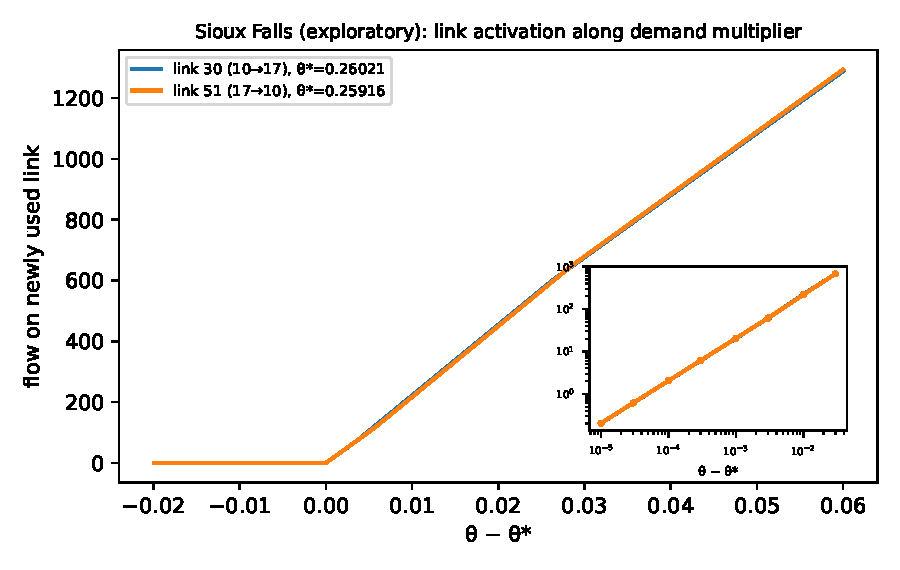
\includegraphics[width=0.78\linewidth]{../figures/sioux_falls.pdf}
\caption{Sioux Falls: flow on a newly used link against $\theta-\theta^*$, with a log--log inset showing linear growth. \status{exploratory}}
\label{fig:sioux}
\end{figure}

\section{Conclusion and open problems}\label{sec:conclusion}

Both questions of Cominetti, Dose and Scarsini have clear answers. For costs whose slope vanishes only at zero load, such as BPR costs, equilibrium link flows remain continuously differentiable while the set of cheapest routes is fixed, at every interior demand level and on every network. A change in that set, however, need not show up as a kink in total cost or the price of anarchy. Five links with standard quartic BPR costs suffice, five is the minimum for a common exponent, and larger networks hide any finite number of derivatives. The slope never jumps in the wrong direction, and for almost every vector of free-flow times it jumps strictly at every nondegenerate nested breakpoint, that is, one at which every edge on a route of the smaller regime is loaded. Exact invisibility is therefore exceptional at such breakpoints. Near-invisibility is robust, because near-matches restore only small kinks, and the new route then carries flows far below what ordinary assignment tolerances resolve.

For practice, the lesson is that kinks in demand curves of total cost or of the price of anarchy are not a reliable detector of route-set changes. Link flows and commodity costs reveal such changes at lower derivative order, and the contact order can be estimated directly.

Open problems:
\begin{enumerate}[nosep]
\item \emph{The endpoint for BPR costs.} Does CDS Theorem~3.2 extend to BPR costs at zero demand, $t_0=0$? Our endpoint counterexample uses oscillating costs.
\item \emph{Degenerate breakpoints.} Is strictness generic at nested breakpoints whose smaller regime contains an unloaded edge?
\item \emph{Mixed exponents.} Do four edges suffice for an equal-slope expansion when BPR exponents differ between edges?
\item \emph{Non-nested breakpoints.} CDS Example~4.8 shows that all slope orders are possible when neither regime contains the other. How smooth can such breakpoints be?
\item \emph{Prevalence.} How often do near-tangent activations occur in calibrated networks, and how small are their kinks? The Sioux Falls test is one data point, and it shows none near nominal demand.
\end{enumerate}


\section*{Declarations}
\addcontentsline{toc}{section}{Declarations}
\textbf{Use of AI tools.} The author used AI tools (large language models) to help develop and check proofs, write and run the verification code, search and check the literature, and draft and edit the text. The author reviewed the results and takes full responsibility for the content.

\textbf{Data and code availability.} No empirical data were collected. The exact verifiers, numerical scripts, generated records and figure sources are in the accompanying reproducibility package, whose \texttt{verify\_all.py} replays every check. The package is archived at Zenodo, doi:\href{https://doi.org/10.5281/zenodo.23552630}{10.5281/zenodo.23552630}, with source at \url{https://github.com/ipitchford/wardrop-smooth-route-regimes}. The Sioux Falls illustration uses the public Transportation Networks for Research data \cite{TNTP,LeBlanc1975}, which are fetched by a script and checked by SHA-256 rather than redistributed.

\textbf{Funding and competing interests.} No specific funding was received. The author declares no competing interests.

\appendix
\section{Several contacts in the two-bank architecture}\label{app:contacts}\label{mc:section}

This appendix counts how many high-order contacts two banks can have and constructs networks with any prescribed finite pattern of them. All statements concern the two-bank architecture. The analytic ingredients are classical Chebyshev systems and Hermite interpolation; the contribution of this section is their physical routing realisation, including positive edge costs, unrestricted directed paths, global bank activity and regularity of the physical optimum. The demand coefficients need not be equal.

\subsection{The local contact law}

The cancellation \eqref{eq:Ecancel} does not need equal commodity demands. The following local statement is used for the contraction of Section~\ref{sec:fiveedge}, for the demand-ratio unfolding and for the repeated transitions below.

\begin{proposition}[Local contact law]\label{prop:localcontact}
Let two fully active parallel banks have analytic effective delays $F,G$ near reference totals $r_Ft_0,r_Gt_0$, where $r_F,r_G,t_0>0$. Give the connector either an analytic nondecreasing cost near zero, or $h(x)=h_0+c x^p$ with $c>0,p>1$. Put
\begin{equation}\label{eq:generalcontact}
 \Delta(t)=F(r_Ft)-G(r_Gt)-h(0),\qquad
 L_0=F'(r_Ft_0)+G'(r_Gt_0)+h'(0)>0.
\end{equation}
Suppose $\Delta(t)=d(t-t_0)^m+O((t-t_0)^{m+1})$, where $d\ne0$ and $m$ is odd. Write $\sigma=\sgn d$, $\delta=t-t_0$, and $\tau=\sigma\delta$. The connector is positive exactly on the side $\tau>0$, and there
\begin{align}
 x(t)&=\frac{|d|}{L_0}\tau^m+o(\tau^m),\label{eq:generalflow}\\
 E(t)-E_0(t)&=-\sigma\frac{t_0m d^2}{L_0}\tau^{2m-1}+o(\tau^{2m-1}),\label{eq:generalcost}\\
 E_0(t)&=r_FtF(r_Ft)+r_GtG(r_Gt).\nonumber
\end{align}
On the other side $x=0$ and $E=E_0$. The remainders have derivative control, so $x\in C^{m-1}\setminus C^m$ and $E\in C^{2m-2}\setminus C^{2m-1}$. The right-minus-left aggregate derivative jump of order $2m-1$ is
\begin{equation}\label{eq:generaljump}
 -\sigma(2m-1)!\frac{t_0m d^2}{L_0}.
\end{equation}
If the physical optimal cost is positive and $C^{2m-1}$ near $t_0$, the same regularity holds for $P$, with this jump divided by $S(t_0)$.
\end{proposition}
\begin{proof}
The connector residual is $F(r_Ft-x)-G(r_Gt+x)-h(x)$, with derivative $-L_0$ at $(t_0,0)$. Its positive root has the first term in \eqref{eq:generalflow}; the sign of $\Delta$ decides whether the root is feasible. At an active equilibrium,
\begin{equation}
 E(t)=r_FtF(r_Ft-x)+r_GtG(r_Gt+x).
\end{equation}
Taylor expansion gives
\begin{equation}\label{eq:raycancellation}
 E-E_0=-t\{r_FF'(r_Ft)-r_GG'(r_Gt)\}x+O(x^2)
       =-t\Delta'(t)x+O(x^2).
\end{equation}
This proves the coefficient in \eqref{eq:generalcost}. For analytic $h$, the signed branch and remainders are analytic. For $h=h_0+cx^p$, divide the residual by $\tau^m$ and write
\begin{equation}
 x=\tau^m U(\tau,\tau^{m(p-1)}),\qquad
 E-E_0=\tau^{2m-1}V(\tau,\tau^{m(p-1)}),
\end{equation}
with $U,V$ analytic and the displayed nonzero leading constants. The implicit-function derivative in $U$ is $-L_0$. Lemma~\ref{lem:remainder} proves the asserted differentiability, including the noninteger-power case. The quotient rule at order $2m-1$ gives the statement for $P$.
\end{proof}

\begin{corollary}[Every positive demand proportion]\label{prop:unequal}
For every $r_F,r_G>0$, the conclusions of Theorem~\ref{thm:main} hold with demands $(r_Ft,r_Gt)$ on the same $m+2$-edge topology, after replacing the original branch operating loads $w_j$ by $r_Fw_j/N$ in $F$ and $r_Gw_j/N$ in $G$. The gap coefficient $a$ is unchanged, and
\begin{equation}
 k_{x;r_F,r_G}=\frac{r_Fr_G\beta}{N(r_F+r_G)}a,
 \qquad k_{E;r_F,r_G}=m a\,k_{x;r_F,r_G}.
\end{equation}
\end{corollary}
\begin{proof}
The scaled bank delays are $F_{r_F}(T)=F(NT/r_F)$ and $G_{r_G}(T)=G(NT/r_G)$, so their inactive gap on this ray is the original $\Delta(t)$. Their total curvature is $L_0=(N/\beta)(1/r_F+1/r_G)$. The residual at $x=0$ is positive for $t>1$, whereas at $x=r_F(t-1)$ the direct delay is $3$ and the shared delay is greater than $2$. Thus $0<x<r_F(t-1)$; both banks stay above their reference loads for all $t>1$. Proposition~\ref{prop:localcontact} and the physical scaling \eqref{eq:optflow} now give every assertion, including analytic $S$.
\end{proof}


\subsection{A zero budget and its equality cases}

Suppose the two fully active banks have demands $r_Ft,r_Gt$, with $r_F,r_G>0$, and tie at $t=1$. Write their reference delays as $\ell_F=\ell_G+h_0$. An edge with reference load $w>0$ and congestion contribution $b_ew^p=1/u$ contributes $w(1+us)^{1/p}$ to its bank throughput at an additional delay $s$. With $\alpha=1/p$, normalise the inverse bank curves by their demand coefficients:
\begin{equation}\label{mc:normalise}
 Q_F(s)=q_F(s)/r_F,\quad Q_G(s)=q_G(s)/r_G,\quad
 \mathcal H(s)=Q_F(s)-Q_G(s)=\sum_{i=0}^{r-1}v_i(1+u_is)^\alpha.
\end{equation}
Let $U$ be the largest physical node before cancellation, so the common fully active latency interval is $I_{\rm phys}=(-1/U,\infty)$. Merge equal nodes and cancel zero net coefficients. If no node remains, $\mathcal H\equiv0$ and there is no isolated contact in this chart. Otherwise $0<u_0<\cdots<u_{r-1}$ and every $v_i\ne0$. The difference $\mathcal H$ extends to $I=(-1/u_{r-1},\infty)\supseteq I_{\rm phys}$; its correspondence with the physical inverse curves is used only on $I_{\rm phys}$.

\begin{lemma}[Classical fractional-power zero bound]\label{mc:chebyshev}
Every nonzero linear combination of $r$ functions $(1+u_is)^\alpha$, with distinct positive $u_i$ and $0<\alpha<1$, has at most $r-1$ zeros on $I$, counted with multiplicity.
\end{lemma}
\begin{proof}
The initial Wronskians have the explicit factorisation
\begin{equation}\label{mc:wronskian}
 W(\phi_0,\ldots,\phi_{n-1})(s)
 =\left(\prod_{k=0}^{n-1}(\alpha)_{\underline{k}}\right)
 \left(\prod_{i<j<n}(u_j-u_i)\right)
 \prod_{i=0}^{n-1}(1+u_is)^{\alpha-n+1}\ne0,
\end{equation}
where $(\alpha)_{\underline{k}}=\alpha(\alpha-1)\cdots(\alpha-k+1)$ and the empty product is one. Indeed, factor $(1+u_is)^\alpha$ from column $i$ and $(\alpha)_{\underline{k}}$ from row $k$, leaving a Vandermonde determinant in $u_i/(1+u_is)$. The standard extended-Chebyshev criterion gives the zero bound; see \cite[Theorem 2.1]{GLT2012}.

For a direct proof of this special case, allow any noninteger exponent $\beta$ and divide $f(s)=\sum_{i=1}^n c_i(1+u_is)^\beta$ by its first basis function. Then
\begin{equation}
 \left(\frac{f}{(1+u_1s)^\beta}\right)'
 =\beta(1+u_1s)^{-\beta-1}
 \sum_{i=2}^n c_i(u_i-u_1)(1+u_is)^{\beta-1}.
\end{equation}
Induction on $n$, followed by Rolle's theorem with multiplicities on a compact interval containing any proposed zeros, gives at most $n-1$ zeros. The exponent remains noninteger at every step and the one-term base case has no zero.
\end{proof}

\begin{proposition}[Contact budget and maximal-contact classification]\label{mc:budget}
Unless $\mathcal H\equiv0$, the isolated zeros of
\begin{equation}
 \Delta(t)=F(r_Ft)-G(r_Gt)-h_0
\end{equation}
for which both inactive bank equilibria are fully active have total multiplicity at most $r-1$. Consequently, contacts of orders $m_1,\ldots,m_\ell$ require at least $1+\sum_jm_j$ physical bank edges, or $2+\sum_jm_j$ edges including the connector.

A nonzero $r$-node difference has contact order $r-1$ at $s=0$ if and only if
\begin{equation}\label{mc:barycentric}
 v_i=\frac{C}{\prod_{k\ne i}(u_i-u_k)},\qquad C\ne0.
\end{equation}
This is its only zero on $I$. If exactly $r$ physical bank edges attain that contact order, their nodes are distinct and their bank assignments alternate in increasing node order; their reference loads divided by the corresponding demand coefficients are proportional to the absolute weights in \eqref{mc:barycentric}.
\end{proposition}
\begin{proof}
A tie corresponds exactly to $t=Q_F(s)=Q_G(s)$. To check its multiplicity, put $d(s)=\Delta(Q_G(s))$. Near a tie,
\begin{equation}\label{mc:unit}
 -\mathcal H(s)=Q_F(s+d(s))-Q_F(s)
 =d(s)\int_0^1Q_F'(s+\theta d(s))\dd\theta.
\end{equation}
The integral is a positive analytic unit, and $Q_G'>0$. Thus the zero orders agree. Lemma~\ref{mc:chebyshev} proves the budget, and the number of surviving nodes cannot exceed the number of physical edges.

Contact order $r-1$ means $\sum_i v_iu_i^k=0$ for $0\le k<r-1$, because the binomial coefficients are nonzero. The $(r-1)\times r$ Vandermonde matrix has a one-dimensional nullspace. Its standard barycentric null vector is \eqref{mc:barycentric}: compare the leading coefficient in the Lagrange interpolant of $u^k$. Its degree-$(r-1)$ moment equals $C\ne0$, so the contact is exact. The zero bound excludes any further zero. Ordered real barycentric weights alternate in sign. With exactly $r$ physical edges there can be no duplicate or cancelled node, proving the equality classification.
\end{proof}

The weights in \eqref{mc:barycentric} and their moment identities are classical interpolation formulas \cite{BT2004,deBoor2005}. The statement is a routing equality classification, not a new barycentric identity. The count concerns fully active banks and does not assert a global lower bound over arbitrary graph topologies. An isolated sign-changing analytic contact is odd, so the five-link example is the first nontransverse case of Proposition~\ref{mc:budget}.

\subsection{Synthesis of any finite pattern of high-order contacts}

\begin{theorem}[Sharp synthesis of prescribed latency contacts]\label{mc:synthesis}
Fix $p>1$, positive $r_F,r_G$, and odd integers $m_1,\ldots,m_\ell\ge3$. Put $M=\sum_jm_j$ and choose any $M+1$ distinct positive nodes $u_0<\cdots<u_M$ and offsets
\begin{equation}
 0=s_1<s_2<\cdots<s_\ell.
\end{equation}
There is an explicit three-vertex, two-commodity network with $M+2$ edges of positive costs $a_e+b_ez^p$ and demands $r_Ft,r_Gt$ such that:
\begin{enumerate}[label=(\roman*),nosep]
\item Its bank edges remain positively loaded for all $t\ge1$. The connector transitions for $t\ge1$ occur exactly at $1=t_1<\cdots<t_\ell$, with $t_j=Q_F(s_j)=Q_G(s_j)$, alternating between contraction and expansion. The final transition may be prescribed as either type.
\item At $t_j$, connector flow lies in $C^{m_j-1}\setminus C^{m_j}$ and equilibrium total cost in $C^{2m_j-2}\setminus C^{2m_j-1}$.
\item If $t_\ell<\gamma=(p+1)^{1/p}$, the physical optimal cost is positive analytic near every $t_j$, and the price of anarchy has the same exact regularity as equilibrium total cost. The explicit sufficient condition $u_Ms_\ell<p$ guarantees this inequality.
\end{enumerate}
The edge count is minimal within the two-bank architecture for the prescribed full-bank contact multiplicities.
\end{theorem}
\begin{proof}
Form the $M\times(M+1)$ confluent matrix
\begin{equation}\label{mc:matrix}
 A_{(j,k),i}=\left.\frac{\mathrm d^k}{\mathrm ds^k}(1+u_is)^\alpha\right|_{s=s_j},
 \qquad 0\le k<m_j,
\end{equation}
with rows ordered by $j$ and then $k$. Every maximal minor is nonzero: a dependence among its $M$ columns would give a nonzero combination with $M$ zeros counted with multiplicity, contradicting Lemma~\ref{mc:chebyshev}.

All these minors have the same sign. Fix an ordered set $I$ of $M$ columns and regard $\det A_I$ as a function of the ordered offsets $s_1<\cdots<s_\ell$ in $I$. It never vanishes, by the zero bound, and the set of ordered offsets is connected, so its sign is constant. To find the sign, let the offsets coalesce: put $s_j=s_*+\epsilon\sigma_j$ with fixed $\sigma_1<\cdots<\sigma_\ell$ and let $\epsilon\downarrow0$. Taylor expansion of each row about $s_*$ gives
\[
 \det A_I=\epsilon^{e}\,\mathcal V(\sigma)\,W_I(s_*)\,(1+o(1)),\qquad e=\binom M2-\sum_j\binom{m_j}2,
\]
where $W_I$ is the Wronskian of $\{\phi_i\}_{i\in I}$ and $\mathcal V(\sigma)=c_{\mathbf m}\prod_{j<k}(\sigma_k-\sigma_j)^{m_jm_k}$ is the confluent Vandermonde determinant, with a constant $c_{\mathbf m}>0$ that depends only on the multiplicities; it is positive for increasing $\sigma$ \cite[Ch.~2]{Karlin1968}. By \eqref{mc:wronskian}, $\sgn W_I=\sgn\prod_{k<M}(\alpha)_{\underline k}$, the same for every $I$ of size $M$. Hence every maximal minor has this sign, without any total positivity assumption beyond \eqref{mc:wronskian}.

Thus the null vector $v_i=(-1)^i\det A_{\widehat i}$ has strictly alternating nonzero entries. Choose its overall sign so that $\widetilde{\mathcal H}(s)=\sum_i v_i(1+u_is)^\alpha$ is negative after the final root for a final expansion, or positive there for a final contraction. The prescribed roots already use the whole $M$-zero budget, so each has exact order $m_j$ and there are no others on $I$. Because $s_1=0$,
\begin{equation}\label{mc:weights}
 C=\sum_{v_i>0}v_i=-\sum_{v_i<0}v_i>0,\qquad
 \lambda_i=|v_i|/C.
\end{equation}
The positive entries specify bank $F$ and the negative entries bank $G$; the $\lambda_i$ in each bank sum to one.

Choose $h_0>0$ and $L>1/u_0$. Set $w_i=r_F\lambda_i$ in $F$ and $w_i=r_G\lambda_i$ in $G$, and give their physical edges the costs
\begin{align}\label{mc:physical}
 c_i^F(z)&=L+h_0-\frac1{u_i}+\frac{z^p}{u_iw_i^p},&&v_i>0,\nonumber\\
 c_i^G(z)&=L-\frac1{u_i}+\frac{z^p}{u_iw_i^p},&&v_i<0,\\
 h(z)&=h_0+z^p.\nonumber
\end{align}
Use the same three-vertex graph as before and permit every directed path. All physical coefficients are positive. The normalised inverse curves are $Q_F=\sum_{v_i>0}\lambda_i\phi_i$ and $Q_G=\sum_{v_i<0}\lambda_i\phi_i$, so the demand thresholds are exactly $t_j=Q_G(s_j)$ and strictly increase from $t_1=1$.

For $t>1$, if $\Delta(t)\le0$ the connector is unused and both banks exceed their reference loads. If $\Delta(t)>0$, its strictly decreasing residual
\begin{equation}\label{mc:residual}
 R(t,x)=F(r_Ft-x)-G(r_Gt+x)-h_0-x^p
\end{equation}
is positive at zero and negative at $x=r_F(t-1)$, since $F(r_F)=L+h_0$, $G(r_G)=L$ and the shared-bank argument has increased. Therefore
\begin{equation}\label{mc:globalbank}
 0<x(t)<r_F(t-1).
\end{equation}
All bank loads remain above their positive reference levels through every interval. The shared loads have the same feasible proportional commodity decomposition as in the original construction. Since $\mathcal H$ and $\Delta$ have opposite signs and all contacts are odd, the connector states alternate with the chosen final orientation. No other bank or connector transition occurs for $t>1$. Bank loads are also positive on a sufficiently small left neighbourhood of $1$.

For the local calculation put $\delta=t-t_j$ and
\begin{equation}\label{mc:localconstants}
 a_j=\frac{\Delta^{(m_j)}(t_j)}{m_j!},\quad
 B_j=Q_F'(s_j)=Q_G'(s_j)>0,\quad
 d_j=\frac1{r_FB_j}+\frac1{r_GB_j}.
\end{equation}
The slopes agree because $m_j\ge3$, and analytic inversion gives
\begin{equation}
 a_j=-\frac{\mathcal H^{(m_j)}(s_j)/m_j!}{B_j^{m_j+1}}\ne0.
\end{equation}
The active side is $a_j\delta>0$. In its positive coordinate $\eta=\sgn(a_j)\delta$, the same two-variable implicit-function argument as in \eqref{eq:twovar} gives
\begin{equation}
 x=\eta^{m_j}U_j(\eta,\eta^{m_j(p-1)}),\qquad
 U_j(0,0)=|a_j|/d_j>0.
\end{equation}
Thus Lemma~\ref{lem:remainder} gives the connector regularity, including real noninteger $p$.

Now $E=t[r_FF(r_Ft-x)+r_GG(r_Gt+x)]$, with analytic inactive continuation $E_0=t[r_FF(r_Ft)+r_GG(r_Gt)]$. Expansion in $x$ yields
\begin{equation}
 E-E_0=-t\Delta'(t)x+O(x^2).
\end{equation}
On the active side its first nonzero term is $-C_j\delta^{2m_j-1}$, where
\begin{equation}\label{mc:costcoefficient}
 C_j=\frac{t_jm_ja_j^2}{d_j}>0.
\end{equation}
The remainder again has the derivative-controlled two-variable form. Hence $E$ has the stated regularity and the exact right-minus-left jump
\begin{equation}\label{mc:costjump}
 E^{(2m_j-1)}(t_j^+)-E^{(2m_j-1)}(t_j^-)
 =-\sgn(a_j)(2m_j-1)!C_j.
\end{equation}

For $t>t_\ell$, the equilibrium load vector is analytic. After a final expansion this follows from positivity of every edge and the scalar analytic implicit-function theorem. After a final contraction the connector is identically zero and both positive banks are analytic. If $t_\ell<\gamma$, all scaled demands $\gamma t_j$ lie in this fixed regime. The physical common-power scaling \eqref{eq:optflow} therefore makes $S$ positive analytic near every transition. Division by $S$ preserves the regularity and divides \eqref{mc:costjump} by $S(t_j)$. Finally,
\begin{equation}
 t_\ell=Q_G(s_\ell)\le(1+u_Ms_\ell)^{1/p}<\gamma
\end{equation}
under the stated sufficient condition. Proposition~\ref{mc:budget} supplies the matching edge lower bound.
\end{proof}

Even contact orders would give isolated tangencies without a change between opposite-side connector regimes. The theorem deliberately prescribes odd orders. Its general construction uses real coefficients; rationality is established separately for the explicit family below.

\subsection{Prescribing demand thresholds locally}

\begin{corollary}\label{mc:prescribeddemand}
Fix the exponent, demand coefficients, nodes and odd contact orders of Theorem~\ref{mc:synthesis}. There is $\varepsilon>0$ such that every ordered demand pattern
\begin{equation}
 1=t_1<t_2<\cdots<t_\ell<1+\varepsilon
\end{equation}
is realised with exactly $2+\sum_jm_j$ positive-cost physical edges and all conclusions of that theorem, including analytic optimal cost at every transition. The cost parameters admit a real-analytic choice near the coincident-threshold limit.
\end{corollary}
\begin{proof}
Use the classical extension of divided differences to repeated nodes \cite{deBoor2005}. For an analytic $\phi(s)=\sum_na_ns^n$,
\begin{equation}\label{mc:divdiffanalytic}
 [z_0,\ldots,z_k]\phi
 =\sum_{n\ge k}a_n h_{n-k}(z_0,\ldots,z_k),
\end{equation}
where $h_d$ is the complete homogeneous symmetric polynomial. The series converges near zero, proving real analyticity in all node arguments, including coincidences. At coincident zero arguments its value is $\phi^{(k)}(0)/k!$.

Replace the rows in \eqref{mc:matrix} by Newton divided-difference rows on successive prefixes of the multiset containing $m_1$ copies of $s_1=0$, then $m_2$ copies of $s_2$, and so on. Their vanishing is equivalent to vanishing of the prescribed Hermite data. The new matrix is analytic even when all $s_j=0$, where its rows become the Taylor rows of orders $0,\ldots,M-1$. Its maximal minors are nonzero there by the Vandermonde formula. Thus its normalised cofactor weights $\lambda_i(s_2,\ldots,s_\ell)$ extend analytically and retain their alternating signs. Their positive and negative masses agree because the first row is $\phi_i(0)=1$.

Choose the overall orientation at the coincident limit so that the sign of $\mathcal H(s)$ for $s>0$ agrees with the prescribed final transition: negative for an expansion and positive for a contraction. This orientation persists for nearby separated contacts: evaluate at a fixed positive point beyond them and use the zero budget. The bank assignments therefore remain fixed. Set
\begin{equation}
 T_j(s)=\sum_{i\in G}\lambda_i(s)(1+u_is_j)^\alpha,\qquad j\ge2.
\end{equation}
At $s=0$ all $T_j=1$. Since $\sum_{i\in G}\lambda_i(s)=1$ identically, the weight-derivative terms vanish there, giving
\begin{equation}
 \frac{\partial T_j}{\partial s_k}(0)=B_0\delta_{jk},\qquad
 B_0=\alpha\sum_{i\in G}\lambda_i(0)u_i>0.
\end{equation}
The analytic inverse-function theorem therefore prescribes any nearby demand vector. Its ordered values imply ordered positive offsets, since each resulting vector uses one strictly increasing function $Q_G$ and $Q_G(0)=1$. Shrink the neighbourhood so that $t_\ell<\gamma$ and all coefficients remain positive. Theorem~\ref{mc:synthesis} applies.
\end{proof}

This is a local existence and analytic parameterisation result. It does not assert a universal explicit radius or rational coefficients for arbitrary target thresholds.

\subsection{Two equal contacts from a factored polynomial}

\begin{theorem}[Closed-form double-contact family]\label{mc:double}
Let $p>1$, let $m\ge3$ be odd, and choose $q>1$ with $q^{p(m+1)}<p+1$. Define
\begin{align}
 n_i&=q^{i+1},\quad u_i=n_i^p-1 &&(0\le i\le2m),\nonumber\\
 V(z)&=\prod_{k=0}^{m-1}(z-q^{pk})(z-q^{1-pk})
       =\sum_{i=0}^{2m}v_iz^i,\label{mc:polynomial}\\
 C&=V(-1)/2,\qquad w_i=|v_i|/C.\nonumber
\end{align}
Put the even-indexed edges in $F$ and the odd-indexed edges in $G$, and use \eqref{mc:physical} with unit demand coefficients. The resulting $2m+2$-edge network has exactly two connector transitions for $t\ge1$: a contraction at $t_1=1$ and an expansion at
\begin{equation}\label{mc:doublethreshold}
 t_2=q^{m+1}.
\end{equation}
Both have contact order $m$. The functions $E$ and $P$ are $C^{2m-2}$ but not $C^{2m-1}$ at both, and $S$ is analytic there. The edge count attains the two-contact lower bound. If $p$ is an integer and $q,L,h_0$ are rational, all physical coefficients are rational.
\end{theorem}
\begin{proof}
The two exponent sets in \eqref{mc:polynomial} are disjoint, since equality would imply $p(k+l)=1$ for nonnegative integers $k,l$. All $2m$ roots are distinct and positive, so $v_i$ has sign $(-1)^i$. The roots include $1$ and $q$; hence $V(1)=V(q)=0$, and the two bank masses both equal $C>0$.

For $\mathcal H(s)=C^{-1}\sum_iv_i(1+u_is)^\alpha$, differentiation at zero through order $m-1$ and expansion of $(n_i^p-1)^k$ give only sums $q^{p l}V(q^{p l})=0$ with $l<m$. At $s=1$,
\begin{equation}
 \phi_i^{(k)}(1)=(\alpha)_{\underline{k}}(n_i^p-1)^kn_i^{1-pk}.
\end{equation}
Expansion gives only sums $q^{1-p l}V(q^{1-p l})=0$ with $l<m$. Thus $0$ and $1$ are contacts of order at least $m$. The $2m$-zero budget makes both orders exact and excludes all other zeros on $I$.

Their orientation is explicit:
\begin{align}
 \mathcal H^{(m)}(0)&=C^{-1}(\alpha)_{\underline m}q^{pm}V(q^{pm})>0,\nonumber\\
 \mathcal H^{(m)}(1)&=-C^{-1}(\alpha)_{\underline m}q^{1-pm}V(q^{1-pm})<0.\label{mc:doublesigns}
\end{align}
The falling factorial is positive for odd $m$; the two evaluations lie respectively above and below all roots of the even-degree polynomial $V$, where $V>0$. Hence $\mathcal H$ is negative below zero, positive between zero and one, and negative above one. The route gap has the opposite sign.

Each paired pair of roots has product $q$, giving
\begin{equation}
 V(q/z)=q^mz^{-2m}V(z),\qquad V(-q)=q^mV(-1).
\end{equation}
The shared bank's normalised throughput at $s=1$ is therefore
\begin{equation}
 t_2=\frac{-q\sum_{i\text{ odd}}v_iq^i}{C}
 =\frac{q[V(-q)-V(q)]}{2C}=q^{m+1}.
\end{equation}
The hypothesis ensures $t_2<\gamma$, and the proof of Theorem~\ref{mc:synthesis} supplies global bank activity and all regularity conclusions. Rationality follows directly from \eqref{mc:polynomial} and \eqref{mc:physical}.
\end{proof}

The factored polynomial is a standard annihilator of geometric moment constraints. Here it gives a compact exact physical example. Choose
\begin{equation}\label{mc:explicitdouble}
 p=4,\quad m=3,\quad q=11/10,\quad L=3,\quad h_0=1.
\end{equation}
Then
\begin{equation}
 V(z)=(z-1)(z-q^4)(z-q^8)(z-q)(z-q^{-3})(z-q^{-7}),
\end{equation}
and the bank costs are $4-u_i^{-1}+z^4/(u_iw_i^4)$ on the four even edges and $3-u_i^{-1}+z^4/(u_iw_i^4)$ on the three odd edges, with connector $1+z^4$. The smallest node is $4641/10000$, so every intercept is positive. The two demand thresholds and boundary costs are
\begin{equation}
 t_1=1,\quad t_2=14641/10000,\qquad
 E(t_1)=7,\quad E(t_2)=131769/10000.
\end{equation}
The integer inequality $11^{16}<5\cdot10^{16}$ certifies $t_2<5^{1/4}$. The exact verifier (Appendix~\ref{app:verification}) reconstructs the physical coefficients, the two cubic contact jets, the rank-six confluent constraints and both nonzero fifth-derivative jumps. The fifth-derivative jumps of $E$, rounded only for display, are $+6.28132652270$ at the contraction and $-0.00155303283209$ at the expansion. The second is about $4{,}000$ times smaller than the first, so after the second contact the hidden transition is even fainter. One eight-edge quartic network thus loses and regains its connector while both aggregate functions remain $C^4$ at both changes.

\section{Proof of the minimality theorem}\label{app:minimality}\label{sec:minimality}

This appendix shows that no network with four or fewer physical edges can have
equal one-sided slopes at a nested breakpoint, whether the minimum-route
regime grows (an expansion) or shrinks (a contraction) as demand increases.
Together with the five-edge examples this shows that five edges are the
minimum for both kinds of breakpoint. The proof is a finite case analysis.
Each case is closed by an explicit inequality, and Table~\ref{tab:minimality}
lists them all.

\subsection{Setting and statement}

We first fix the class of networks and the kind of breakpoint we study.

\begin{definition}[Standing class]\label{def:standing}
A \emph{network in the standing class} consists of:
\begin{enumerate}
\item a finite directed multigraph $\Gamma$ with vertex set $V$ and edge set
 $\mathcal E$ (parallel and antiparallel edges are allowed);
\item for each edge $e$, a cost $c_e(z)=a_e+b_ez^p$ for $z\ge0$, with
 $a_e,b_e>0$ and one real exponent $p>1$ common to all edges;
\item finitely many commodities $k$, each with an origin $o_k$, a destination
 $d_k\ne o_k$, and demand $tr_k$, where $r_k>0$ and $t>0$ is the scale
 parameter.
\end{enumerate}
The routes of commodity $k$ are \emph{all} simple directed $o_k$--$d_k$
paths in $\Gamma$; we assume there is at least one. We identify a route $P$
with its edge-incidence vector $1_P\in\{0,1\}^{\mathcal E}$. A route is
determined by its edge set, since it is simple.
\end{definition}

A Wardrop equilibrium at scale $t$ is a nonnegative route flow meeting the
demands in which every route with positive flow has minimum cost among the
routes of its commodity. Because every $c_e$ is strictly increasing, the
aggregate edge load $z(t)\in\R^{\mathcal E}_{\ge0}$ of an equilibrium is
unique. Its equilibrium total cost is
\[
 E(t)=\sum_{e}z_e(t)\,c_e(z_e(t)),
\]
and $S(t)$ denotes the minimum of the same total cost over all feasible
route flows. The price of anarchy is $P(t)=E(t)/S(t)$.

We need the set of cheapest routes, not merely the set of used routes.

\begin{definition}[Regimes and nested breakpoints]\label{def:regimeB}
For a load vector $z$, the \emph{complete minimum-route set} $R_k(z)$ of
commodity $k$ is the set of all routes of $k$ whose cost under $c(z)$ is
minimal. It depends only on $z$, not on any route decomposition of $z$. The
\emph{regime} at scale $t$ is the family $R(t)=(R_k(z(t)))_k$. For families we
write $R\subseteq R'$ if $R_k\subseteq R'_k$ for every $k$, and
$R\subsetneq R'$ if moreover the inclusion is strict for some $k$.

A scale $t_0>0$ is a \emph{nested breakpoint} if there is $\varepsilon>0$ such
that $R(t)=R_-$ for $t\in(t_0-\varepsilon,t_0)$ and $R(t)=R_+$ for
$t\in(t_0,t_0+\varepsilon)$, and either
\begin{itemize}
\item $R_-\subsetneq R_+$ (an \emph{expansion}), or
\item $R_+\subsetneq R_-$ (a \emph{contraction}).
\end{itemize}
In either case $R_s$ denotes the smaller and $R_l$ the larger of the two
regimes. The \emph{smaller side} is the punctured one-sided neighbourhood on
which $R(t)=R_s$: it is the left side for an expansion and the right side for
a contraction. The other side is the \emph{larger side}.
\end{definition}

For a family $R$ of route sets let
\[
 \mathcal K_R=\operatorname{span}\{1_P-1_Q:\ P,Q\in R_k\text{ for some }k\}.
\]
This is the set of aggregate edge images of signed route flows on $R$ that
leave every commodity's total demand unchanged. Every element of
$\mathcal K_R$ has zero net flow at every vertex, so $\mathcal K_R$ lies in
the incidence kernel $\mathcal K(\Gamma)$ of $\Gamma$. For a weakly connected
multigraph with $n$ vertices and $e$ edges, $\dim\mathcal K(\Gamma)=e-n+1$.

\begin{theorem}[Four-edge lower bound]\label{thm:fouredge}
Let a network in the standing class have at most four physical edges, and
let $t_0>0$ be a nested breakpoint. Then both one-sided derivatives of $E$
and of $P$ exist at $t_0$, and
\begin{align*}
 E'(t_0^-)&>E'(t_0^+),\quad P'(t_0^-)>P'(t_0^+)
 &&\text{for an expansion},\\
 E'(t_0^-)&<E'(t_0^+),\quad P'(t_0^-)<P'(t_0^+)
 &&\text{for a contraction}.
\end{align*}
\end{theorem}

\begin{corollary}[Minimality of five edges]\label{cor:fiveminimal}
In the standing class, five is the minimum number of physical edges for
which equal one-sided slopes of $E$ (equivalently of $P$) occur at a nested
expansion, and five is also the minimum for a nested contraction.
\end{corollary}

\begin{proof}
Theorem~\ref{thm:fouredge} excludes four or fewer edges. Five edges suffice
for expansions by Theorem~\ref{thm:main}, and for contractions by the
bank-swapped five-edge contraction of Section~\ref{sec:fiveedge}.
\end{proof}

\subsection{General tools}

We use the weak slope comparison, Theorem~\ref{thm:weakcomparison}, and the tangency lemma, Lemma~\ref{lem:tangencycomparison}. Costs in the standing class satisfy their hypotheses: $c_e'(z)=pb_ez^{p-1}$ is continuous on $[0,\infty)$ and positive for $z>0$, and $c_e\ge a_e>0$. For an expansion the smaller side is the left one, so \eqref{eq:distancejump} reads $E'(t_0^-)\ge E'(t_0^+)$; for a contraction it reads $E'(t_0^+)\ge E'(t_0^-)$. Theorem~\ref{thm:fouredge} for $E$ is thus the assertion that the equality $Dv_s=Dv_l$ is impossible. We call this equality \emph{slope equality}. By Lemma~\ref{lem:tangencycomparison}, if $P\in R_{l,k}\setminus R_{s,k}$ and $Q\in R_{s,k}$, then $g(t)=c(z(t))^T(1_P-1_Q)$ is positive on the smaller side, vanishes at $t_0$, and under slope equality has zero one-sided derivative there from the smaller side.

Two symmetries let us halve several case distinctions. The first reverses
all traffic.

\begin{lemma}[Reversal symmetry]\label{lem:reversal}
Let $\Gamma^{\mathrm{rev}}$ be obtained by reversing every edge, with the same
costs, and give each commodity the origin $d_k$ and destination $o_k$ and the
same demand. Then $P\mapsto P^{\mathrm{rev}}$ (traverse in the opposite
direction) is a cost-preserving bijection between the routes of $k$ in the
two networks, with $1_{P^{\mathrm{rev}}}=1_P$. Consequently both networks
have the same equilibrium edge loads at every scale, corresponding regimes,
the same spaces $\mathcal K_R$, and the same functions $E$ and $S$. Nested
breakpoints, their type (expansion or contraction) and their one-sided
slopes correspond.
\end{lemma}

\begin{proof}
A sequence of edges is a simple directed $o_k$--$d_k$ path in $\Gamma$
exactly when the reversed sequence is a simple directed $d_k$--$o_k$ path in
$\Gamma^{\mathrm{rev}}$, and both use the same edges. Hence the incidence
vectors of the route sets agree, so the sets of feasible aggregate loads
agree and route costs agree under every load vector. The Wardrop conditions
and the complete minimum-route sets are statements about these costs, and
$E$ and $S$ depend only on loads. All claims follow.
\end{proof}

The second symmetry is relabelling: renaming vertices and edges by an
isomorphism of multigraphs, with costs and commodities carried along, changes
nothing. We use the composite of reversal with a relabelling, which we call
the \emph{exchange symmetry}; it is described in
Lemma~\ref{lem:sides}\,(e).

Next we reduce to connected graphs and to one commodity per endpoint pair.

\begin{lemma}[Reductions]\label{lem:reductions}
In proving Theorem~\ref{thm:fouredge} we may assume that $\Gamma$ has no
loops, is weakly connected, and has at most one commodity for each ordered
pair of endpoints.
\end{lemma}

\begin{proof}
A loop lies on no simple path; it carries no load and can be deleted, which
does not increase the edge count. If $\Gamma$ has several weak components,
each commodity lives in one of them, and the equilibrium, the regime, $E$ and
$\mathcal K_R$ split as direct sums over components. Every component inherits
constant regimes on both punctured sides, nested in the same direction. On a
component whose regime does not change, the weak comparison theorem with
$R_s=R_l$ gives equal one-sided slopes. Every component whose regime changes
has at most four edges and a nested breakpoint of the same type. If the
inequality of Theorem~\ref{thm:fouredge} is strict for each such component,
adding the components gives strictness for $E$. Finally, commodities with
the same endpoints have the same routes and the same minimum cost; merging
them into one commodity with the summed demand changes neither the
equilibrium loads nor the regimes, nor $E$ or $S$.
\end{proof}

The dimension lemma disposes of every graph whose incidence kernel is at most
one-dimensional.

\begin{lemma}[Dimension lemma]\label{lem:dimension}
At a nested breakpoint of either type, $\mathcal K_{R_s}\subsetneq
\mathcal K_{R_l}$. If $\mathcal K_{R_s}=\{0\}$, slope equality fails, on any
graph in the standing class.
\end{lemma}

\begin{proof}
Choose $k$, $P\in R_{l,k}\setminus R_{s,k}$ and $Q\in R_{s,k}$, and put
$\kappa=1_P-1_Q\in\mathcal K_{R_l}$. On the smaller side, all routes in
$R_{s,k}$ have equal cost, so $c(z(t))$ is orthogonal to $\mathcal K_{R_s}$.
If $\kappa\in\mathcal K_{R_s}$, then $P$ would cost the same as $Q$ there and
would be cheapest, which is false. Hence $\kappa\notin\mathcal K_{R_s}$.

Now let $\mathcal K_{R_s}=\{0\}$. Then all routes in $R_{s,k}$ have the same
incidence vector, so each commodity has a single cheapest route $Q_k$ on the
smaller side and carries its whole demand there. Thus $z(t)=tq$ on the
smaller side, with $q=\sum_kr_k1_{Q_k}=z_0/t_0$, and $q+\mathcal K_{R_s}=\{q\}$
gives $v_s=q$. Suppose slope equality holds. Lemma~\ref{lem:tangencycomparison} gives
$(Dv_s)^T\kappa=(Dq)^T\kappa=0$, and $c_0^T\kappa=0$ because $g(t_0)=0$. For
every edge, $c_e'(z)z=pb_ez^p=p(c_e(z)-a_e)$, also at $z=0$. Hence
\[
 Dq=\frac p{t_0}(c_0-a),
\]
so $(c_0-a)^T\kappa=0$ and then $a^T\kappa=0$. Since
$c_e(tq_e)=a_e+(t/t_0)^p(c_{0,e}-a_e)$,
\[
 c(tq)^T\kappa=a^T\kappa+(t/t_0)^p(c_0-a)^T\kappa=0
\]
for all $t$. On the smaller side $P$ would therefore be cheapest, a
contradiction.
\end{proof}

The parallel-bank lemmas treat a set of parallel edges carrying a fixed total
flow.

\begin{definition}[Banks]\label{def:bank}
A \emph{bank} is a set of $m\ge1$ parallel edges with a common tail and head
and costs $c_i=a_i+b_iz^p$. For a total flow $T\ge0$, the bank equilibrium
assigns loads $x_i\ge0$ with $\sum_ix_i=T$ such that all loaded edges have a
common cost $\ell(T)$, the \emph{effective latency}, and every unloaded edge
has free-flow cost at least $\ell(T)$. The \emph{minimum set} is
$M(T)=\{i:\ a_i\le\ell(T)\}$, the set of edges whose cost equals the minimum.
\end{definition}

The bank equilibrium is explicit: with
$N(\lambda)=\sum_i\bigl((\lambda-a_i)_+/b_i\bigr)^{1/p}$, which is continuous,
zero at $\lambda=\min_ia_i$ and strictly increasing for larger $\lambda$,
$\ell(T)$ is the unique $\lambda\ge\min_ia_i$ with $N(\lambda)=T$, and
$x_i=((\ell-a_i)_+/b_i)^{1/p}$. The next lemma records how the latency
behaves near a given flow.

\begin{lemma}[Single bank]\label{lem:bank}
Let $T_0>0$, $\lambda_0=\ell(T_0)$, $I=\{i:a_i<\lambda_0\}$ (the positively
loaded edges, nonempty) and $J=\{j:a_j=\lambda_0\}$. Put
$d_i=c_i'(x_i)>0$ for $i\in I$ and $\eta=\sum_{i\in I}d_i^{-1}$.
\begin{enumerate}
\item[(a)] $\ell$ is continuous and strictly increasing, so $M(T)$ is
 nondecreasing in $T$ for inclusion: branches only join as flow grows.
\item[(b)] $\ell$ has left derivative $\ell'(T_0^-)=\eta^{-1}>0$.
\item[(c)] If $J=\emptyset$, then $\ell$ is real-analytic near $T_0$ with
 $\ell'(T_0)=\eta^{-1}$. If $J\ne\emptyset$, the right derivative is
 $\ell'(T_0^+)=0$.
\end{enumerate}
\end{lemma}

\begin{proof}
(a) $N$ is a continuous strictly increasing bijection from
$[\min_ia_i,\infty)$ onto $[0,\infty)$, so its inverse $\ell$ is continuous
and strictly increasing, and $\{i:a_i\le\ell(T)\}$ grows with $T$.

(b), (c) Near $\lambda_0$, $N(\lambda)=N_I(\lambda)+N_J(\lambda)$ with
$N_I(\lambda)=\sum_{i\in I}((\lambda-a_i)/b_i)^{1/p}$ real-analytic near
$\lambda_0$, $N_I'(\lambda_0)=\eta$ (because $dx_i/d\lambda=1/c_i'(x_i)$), and
$N_J(\lambda)=\sum_{j\in J}((\lambda-\lambda_0)_+/b_j)^{1/p}$, which vanishes
for $\lambda\le\lambda_0$. Hence $\ell=N_I^{-1}$ to the left of $T_0$, which
gives (b), and also to the right when $J=\emptyset$, which gives the first
part of (c). If $J\ne\emptyset$, put $C=\sum_{j\in J}b_j^{-1/p}>0$. For
$T>T_0$ and $\lambda=\ell(T)>\lambda_0$, monotonicity of $N_I$ gives
$T-T_0\ge C(\lambda-\lambda_0)^{1/p}$, so
$0<\ell(T)-\lambda_0\le((T-T_0)/C)^p=o(T-T_0)$, since $p>1$.
\end{proof}

The curvature lemma compares the effective latency of a bank with a single
common-power edge.

\begin{lemma}[Parallel-bank curvature]\label{lem:curvature}
Let $\ell$ be the effective latency of a bank and let $T>0$ be such that all
$m$ edges are positively loaded, $x_i>0$. Put $d_i=c_i'(x_i)$ and
$\eta=\sum_id_i^{-1}$. Then
\begin{equation}\label{eq:min_curv}
 \ell''(T)-\frac{p-1}{T}\ell'(T)
 =\frac{p-1}{T\eta^3}\Bigl[T\sum_i\frac1{x_id_i^2}-\eta^2\Bigr]\ge0,
\end{equation}
with equality exactly when all offsets $a_i$ are equal. In that case
$\ell(T)=a+\kappa T^p$ for all $T\ge0$, with $a$ the common offset and
$\kappa=(\sum_ib_i^{-1/p})^{-p}$.
\end{lemma}

\begin{proof}
With all edges loaded, $T=N(\lambda)$ with
$N'(\lambda)=\sum_i1/c_i'(x_i)=\eta$ and
$N''(\lambda)=-\sum_ic_i''(x_i)/c_i'(x_i)^3$. For common-power costs
$c_i''(x)=(p-1)c_i'(x)/x$ when $x>0$, so
$N''=-(p-1)\sum_i1/(x_id_i^2)$. Inverse differentiation gives
$\ell'=1/N'=\eta^{-1}$ and
\[
 \ell''=-\frac{N''}{(N')^3}=\frac{p-1}{\eta^3}\sum_i\frac1{x_id_i^2}.
\]
Subtracting $(p-1)\ell'/T=(p-1)\eta^2/(T\eta^3)$ gives the identity in
\eqref{eq:min_curv}. By the Cauchy--Schwarz inequality,
\[
 \eta^2=\Bigl(\sum_i\sqrt{x_i}\cdot\frac1{\sqrt{x_i}\,d_i}\Bigr)^2
 \le\Bigl(\sum_ix_i\Bigr)\sum_i\frac1{x_id_i^2}=T\sum_i\frac1{x_id_i^2},
\]
with equality exactly when $x_i d_i$ is the same for all $i$. Since
$x_id_i=pb_ix_i^p=p(\ell(T)-a_i)$, this means all $a_i$ are equal. If
$a_i=a$ for all $i$, then $x_i=((\ell-a)/b_i)^{1/p}$ and summing gives
$T=(\ell-a)^{1/p}\sum_ib_i^{-1/p}$, which is the stated formula.
\end{proof}

We use the lemma through the operator $\mathcal L[\varphi](t)=\varphi''(t)-
(p-1)\varphi'(t)/t$ on functions of $t>0$. It annihilates $\alpha+\beta t^p$
for all constants $\alpha,\beta$. If $Q>0$ and all bank edges are positively
loaded at $T=Qt$, the function $\ell_Q(t)=\ell(Qt)$ satisfies
\begin{equation}\label{eq:min_tcurv}
 \mathcal L[\ell_Q](t)=Q^2\Bigl[\ell''(Qt)-\frac{p-1}{Qt}\ell'(Qt)\Bigr]>0
 \quad\text{unless all offsets are equal.}
\end{equation}
If $\varphi(t_0)=\varphi'(t_0)=0$, then $\varphi''(t_0)=\mathcal L[\varphi](t_0)$.

The next lemma disposes of every network whose underlying graph is a tree.

\begin{lemma}[Trees of parallel banks]\label{lem:tree}
Suppose that the underlying simple undirected graph of $\Gamma$ (obtained by
merging parallel and antiparallel edges) is a tree. Then no nested
contraction occurs, and at every nested expansion
$E'(t_0^-)>E'(t_0^+)$.
\end{lemma}

\begin{proof}
For an ordered pair $(x,y)$ of adjacent vertices, the edges from $x$ to $y$
form a bank $\mathcal B_{xy}$. Every commodity $k$ has a unique vertex
sequence, namely the tree path from $o_k$ to $d_k$, and its routes are
exactly the choices of one edge from each bank along that sequence; all such
choices are simple paths and hence available. The bank $\mathcal B_{xy}$
therefore carries the total flow $Q_{xy}t$, where $Q_{xy}$ is the sum of the
$r_k$ over commodities whose sequence traverses $x$ then $y$. The
equilibrium splits each bank independently as a bank equilibrium, because a
route's cost is the sum of the costs of its bank edges. A route is cheapest
exactly when each of its edges lies in the minimum set of its bank. Thus
$R_k(t)$ is the product of the sets $M_{xy}(Q_{xy}t)$ along the sequence of
$k$, and the regime is nondecreasing in $t$ by Lemma~\ref{lem:bank}(a). This
excludes $R_+\subsetneq R_-$.

At an expansion, every bank with $Q_{xy}>0$ has minimum sets $M_-\subseteq
M_+$ on the two sides (the product of nonempty sets is monotone in each
factor), and at least one such bank has $M_-\subsetneq M_+$. Fix a bank with
$Q=Q_{xy}>0$ and $M_-\subsetneq M_+$, and write $T_0=Qt_0$ and
$\lambda_0=\ell(T_0)$. If $i\in M_-$ then $a_i\le\ell(Qt)<\lambda_0$ for
$t<t_0$; if $j\in M_+\setminus M_-$ then $a_j>\ell(Qt)$ for $t<t_0$ and
$a_j\le\ell(Qt)$ for $t>t_0$, so $a_j=\lambda_0$. In the notation of
Lemma~\ref{lem:bank}, $I=M_-$ and $J=M_+\setminus M_-\ne\emptyset$. The bank
contributes $E_{xy}(t)=Qt\,\ell(Qt)$ to $E$, so by Lemma~\ref{lem:bank}(b,c)
\[
 E_{xy}'(t_0^-)-E_{xy}'(t_0^+)=Q^2t_0\bigl[\ell'(T_0^-)-\ell'(T_0^+)\bigr]
 =Q^2t_0\eta^{-1}>0.
\]
For a bank whose minimum set $M$ does not change, the same argument shows
$a_i<\lambda_0$ for $i\in M$ and $a_i>\lambda_0$ otherwise, so $J=\emptyset$
and its contribution has a continuous derivative by
Lemma~\ref{lem:bank}(c). Summing over banks gives the claim.
\end{proof}

We also need that a single commodity's cost increases with its demand.

\begin{lemma}[Monotone single-commodity cost]\label{lem:monotone}
If all commodities share the same endpoints and are merged into one
commodity of demand $Rt$, its equilibrium cost $\lambda(t)$ is strictly
increasing in $t$.
\end{lemma}

\begin{proof}
Let $t_1<t_2$, with loads $z_i=z(t_i)$ and costs $\lambda_i$. Every route
costs at least $\lambda_i$ under $c(z_i)$, and the used routes cost exactly
$\lambda_i$. Decomposing $z_j$ into routes therefore gives
$c(z_i)^Tz_j\ge\lambda_iRt_j$ and $c(z_i)^Tz_i=\lambda_iRt_i$. Hence
\[
 0\le(c(z_2)-c(z_1))^T(z_2-z_1)\le(\lambda_2-\lambda_1)R(t_2-t_1).
\]
If $\lambda_2\le\lambda_1$, the middle expression vanishes, so $z_1=z_2$ by
strict monotonicity of the costs. This is impossible, because the total flow
leaving the origin is $Rt_1$ for one load and $Rt_2$ for the other.
\end{proof}

\subsection{The transitive triangle with a duplicated side}

After the general tools, only one family of graphs remains. The next lemma
identifies it.

\begin{lemma}[Graph reduction]\label{lem:graphs}
Let $\Gamma$ be loopless and weakly connected with $n$ vertices and $e\le4$
edges, and suppose its underlying simple graph is not a tree. If
$\dim\mathcal K(\Gamma)\le1$, a nested breakpoint has
$\mathcal K_{R_s}=\{0\}$. Otherwise $n=3$, $e=4$, and if
$\dim\mathcal K_{R_s}\ge1$ then $\mathcal K_{R_l}=\mathcal K(\Gamma)$ and
$\Gamma$ is a \emph{transitive triangle with one duplicated side}: up to
relabelling, its vertices are $s,u,v$, it has one edge on each of the sides
$s\to v$, $s\to u$, $u\to v$, and one further edge parallel to one of them.
\end{lemma}

\begin{proof}
$\dim\mathcal K(\Gamma)=e-n+1$. If $n\ge4$, this is at most $1$. If $n=2$,
the underlying simple graph is a single edge, a tree. If $n=3$ and $e\le3$, it
is at most $1$. When it is at most one, the strict inclusion
$\mathcal K_{R_s}\subsetneq\mathcal K_{R_l}\subseteq\mathcal K(\Gamma)$ of
Lemma~\ref{lem:dimension} forces $\mathcal K_{R_s}=\{0\}$. Hence the only
remaining case is $n=3$, $e=4$, $\dim\mathcal K(\Gamma)=2$. If
$\dim\mathcal K_{R_s}\ge1$, the strict inclusion forces
$\mathcal K_{R_l}=\mathcal K(\Gamma)$.

The cost vector $c_0$ is orthogonal to $\mathcal K_{R_l}$, being the limit of
cost vectors orthogonal to it on the larger side. The incidence vector of a
directed cycle lies in $\mathcal K(\Gamma)=\mathcal K_{R_l}$, but its inner
product with $c_0>0$ is positive. Hence $\Gamma$ has no directed cycle, and
in particular no pair of antiparallel edges. An acyclic graph on three
vertices has a topological order $s<u<v$ with every edge going forward. The
underlying simple graph is not a tree, so all three pairs are joined; their
multiplicities are positive and sum to four, so they are $2,1,1$ in some
order.
\end{proof}

For the rest of this subsection $\Gamma$ is a transitive triangle with one
duplicated side. Its \emph{sides} are $f$ ($s\to v$), $h$ ($s\to u$) and $g$
($u\to v$). The duplicated side $\sigma^*$ has two edges $e_1,e_2$; each other
side has one edge, also denoted $f$, $h$ or $g$. Only the endpoint pairs
$(s,v)$, $(s,u)$, $(u,v)$ are joined by directed paths. By
Lemma~\ref{lem:reductions} there is at most one commodity per pair; we write
$R,A,B\ge0$ for the demand coefficients of $s\to v$, $s\to u$, $u\to v$,
with a zero coefficient meaning that the commodity is absent. The routes are
single edges of side $h$ (for $s\to u$) or $g$ (for $u\to v$); and for
$s\to v$ the \emph{direct} routes (one edge of side $f$) and the
\emph{indirect} routes (one edge of side $h$ followed by one edge of side
$g$).

The next lemma describes regimes through side minima; it is where
availability of all simple paths is used.

\begin{lemma}[Side structure and aggregation]\label{lem:sides}
Fix a load vector $z$. For each side $\sigma$ let $m_\sigma$ be the least
cost among its edges and $M_\sigma$ the set of edges attaining it. Put
$\varpi=m_h+m_g-m_f$.
\begin{enumerate}
\item[(a)] $R_{su}=M_h$ and $R_{uv}=M_g$ (when present), and
 $R_{sv}=M_f$ if $\varpi>0$, $R_{sv}=M_h\times M_g$ if $\varpi<0$, and
 $R_{sv}=M_f\cup(M_h\times M_g)$ if $\varpi=0$.
\item[(b)] An edge outside $M_\sigma$ carries zero load in any equilibrium.
\item[(c)] If the sign of $\varpi$ is nonzero and fixed, the side loads
 $y_\sigma=\sum_{e\in\sigma}z_e$ of an equilibrium at scale $t$ are
 $(y_f,y_h,y_g)=(R,A,B)t$ when $\varpi>0$ and $(0,A+R,B+R)t$ when $\varpi<0$.
\item[(d)] If a route of commodity $k$ is not cheapest, its excess cost over
 the cheapest route of $k$ is $m_\sigma'-m_\sigma$ when it uses a
 non-minimum edge of cost $m_\sigma'$ on a side $\sigma$ and otherwise
 follows cheapest edges, and it is $|\varpi|$ when it is a direct (resp.\
 indirect) route built from cheapest edges while $\varpi<0$ (resp.\
 $\varpi>0$). In particular, all such routes of the same kind have the same
 excess, whichever edge of a bank with equal costs they use.
\item[(e)] (Exchange symmetry.) Reversal (Lemma~\ref{lem:reversal}) followed
 by the relabelling $s\leftrightarrow v$ maps the network to a transitive
 triangle with one duplicated side in which the roles of $(h,A)$ and $(g,B)$
 are exchanged and $f$ and $R$ are unchanged; it preserves the type of
 every breakpoint, the regimes' sign of $\varpi$, and the slopes of $E$.
\end{enumerate}
\end{lemma}

\begin{proof}
(a) Every combination of an $h$-edge and a $g$-edge is a simple
$s\to v$ path and is available. The cheapest $s\to u$ and $u\to v$ routes are
therefore the cheapest edges of the corresponding side, the cheapest
indirect routes are the pairs in $M_h\times M_g$ with cost $m_h+m_g$, and the
cheapest direct routes are $M_f$ with cost $m_f$. Comparing $m_f$ with
$m_h+m_g$ gives (a).

(b) If an edge $e$ of side $\sigma$ carries load, some used route contains
it, and replacing $e$ by an edge of $M_\sigma$ gives an available route that
is strictly cheaper unless $e\in M_\sigma$.

(c) If $\varpi>0$, all $s\to v$ flow is direct, and if $\varpi<0$ it is all
indirect; the other commodities have routes inside a single side.

(d) This is the computation in (a).

(e) Reversal turns $s\to u$, $u\to v$, $s\to v$ into $u\to s$, $v\to u$,
$v\to s$. After renaming $s\leftrightarrow v$ these read $u\to v$, $s\to u$,
$s\to v$: the old side $g$ becomes the new side $h$ and conversely, and the
old $s\to u$ commodity becomes the new $u\to v$ commodity. Direct routes stay
direct. Lemma~\ref{lem:reversal} gives the remaining assertions.
\end{proof}

Write $\pi=1_{e_2}-1_{e_1}$ and, for edges $\varphi,\chi,\psi$ of the sides
$f,h,g$, let $\tau(\varphi,\chi,\psi)=1_\chi+1_\psi-1_\varphi$ be a
\emph{triangle difference}. Two triangle differences are equal or differ by
$\pm\pi$. We say that the duplicated side is \emph{active} in a regime if
some route of the regime uses an edge of $\sigma^*$.

The classification lemma lists the possible route-difference spaces.

\begin{lemma}[Route-space classification]\label{lem:routespaces}
$\mathcal K(\Gamma)$ is two-dimensional and is spanned by $\pi$ and any
triangle difference. For any family $R$ of nonempty route sets,
$\mathcal K_R$ is spanned by vectors each of which is $\pm\pi$ or a triangle
difference; hence if $\dim\mathcal K_R=1$, either $\mathcal K_R=
\operatorname{span}\{\pi\}$ or $\mathcal K_R=\operatorname{span}\{\tau\}$ for
a single triangle difference $\tau$. For a complete regime with data
$M_\sigma,\varpi$ as in Lemma~\ref{lem:sides}:
\begin{enumerate}
\item[(a)] $\pi\in\mathcal K_R$ if and only if $\sigma^*$ is active and
 $M_{\sigma^*}=\{e_1,e_2\}$;
\item[(b)] $\mathcal K_R$ contains a triangle difference if and only if
 $R>0$ and $\varpi=0$;
\item[(c)] $\dim\mathcal K_R$ is the number of conditions among (a), (b)
 that hold, and when only (b) holds, $\mathcal K_R=\operatorname{span}\{\tau\}$
 where $\tau$ is built from the unique cheapest edge of each side.
\end{enumerate}
\end{lemma}

\begin{proof}
$\dim\mathcal K(\Gamma)=4-3+1=2$, and $\pi$ and a triangle difference are
independent elements of it, since a triangle difference has three nonzero
entries on three different sides while $\pi$ is supported on one side.
The generators $1_P-1_Q$ of $\mathcal K_R$ are differences of two routes of
one commodity. For $s\to u$ or $u\to v$ they are $0$ or $\pm\pi$. For
$s\to v$, two direct routes or two indirect routes differ by $0$ or $\pm\pi$,
and a direct and an indirect route differ by a triangle difference. If
$\dim\mathcal K_R=1$, either every nonzero generator is $\pm\pi$, or some
generator is a triangle difference $\tau$; in the latter case no generator is
$\pm\pi$ (which is not a multiple of $\tau$), and a second, different
triangle difference would differ from $\tau$ by $\pm\pi$ and raise the
dimension.

For a complete regime, routes use only edges of the sets $M_\sigma$, and by
Lemma~\ref{lem:sides}(a) every combination of such edges compatible with
the sign of $\varpi$ is a route of the regime. If $\sigma^*$ is active and
$|M_{\sigma^*}|=2$, a route through $e_1$ and the same route through $e_2$
both lie in the regime, so $\pi\in\mathcal K_R$. Otherwise all routes of the
regime use a fixed edge on each side, and $\mathcal K_R$ is contained in the
span of the single triangle difference $\tau$ built from these edges, which
does not contain $\pi$. This proves (a). A triangle difference is a
generator exactly when $s\to v$ has both a cheapest direct and a cheapest
indirect route, that is $R>0$ and $\varpi=0$; if this fails, every generator
is $0$ or $\pm\pi$. This proves (b), and (c) follows.
\end{proof}

In the remaining two lemmas $\Gamma$ is a transitive triangle with one
duplicated side, $t_0$ is a nested breakpoint of either type,
$\dim\mathcal K_{R_s}=1$ and $\mathcal K_{R_l}=\mathcal K(\Gamma)$. By
Lemma~\ref{lem:routespaces}, the larger regime has $R>0$, $\varpi=0$, both
$e_1,e_2$ cheapest and $\sigma^*$ active. By the same lemma, the smaller
regime has one of two types:
\begin{description}
\item[Type P] (old cycle is the parallel pair) $\mathcal K_{R_s}=
 \operatorname{span}\{\pi\}$: on the smaller side $\sigma^*$ is active with
 both edges cheapest, and $\varpi\ne0$.
\item[Type T] (old cycle is the triangle) $\mathcal K_{R_s}=
 \operatorname{span}\{\tau\}$: on the smaller side $\varpi=0$, and exactly one
 edge of $\sigma^*$, say $e_1$, is cheapest.
\end{description}
In type~P the sign of $\varpi$ on the smaller side is constant, because
$R_{sv}$ is either a set of direct routes or a set of indirect routes; we
call the \emph{old long route} direct if $\varpi>0$ and indirect if
$\varpi<0$ there.

\begin{lemma}[Old cycle is the parallel pair]\label{lem:typeP}
In type~P, slope equality fails, for expansions and for contractions.
\end{lemma}

\begin{proof}
\emph{Set-up.} By Lemma~\ref{lem:sides}(c), on the smaller side the side
loads are $y_\sigma(t)=Q_\sigma t$, with $(Q_f,Q_h,Q_g)=(R,A,B)$ for a direct
old long route and $(0,A+R,B+R)$ for an indirect one. The bank
$\sigma^*=\{e_1,e_2\}$ is active, so $Q:=Q_{\sigma^*}>0$; let $\ell$ be its
effective latency, $T_0=Qt_0$ and $\lambda_0=\ell(T_0)$. If the old long
route is indirect, side $f$ carries no load and is not on any route of
$R_s$, so $\sigma^*\ne f$. Hence $\sigma^*=f$ forces a direct old long
route. By the exchange symmetry (Lemma~\ref{lem:sides}(e)) we may assume
$\sigma^*\in\{f,g\}$; for $\sigma^*=g$ with a direct old long route, activity
means $B>0$.

For $t$ near $t_0$ define the \emph{gap}
\[
 G(t)=
 \begin{cases}
 c_h(At)+c_g(Bt)-\ell(Rt), & \sigma^*=f\ \text{(direct)},\\
 a_f-c_h((A+R)t)-\ell((B+R)t), & \sigma^*=g,\ \text{indirect},\\
 c_h(At)+\ell(Bt)-c_f(Rt), & \sigma^*=g,\ \text{direct}.
 \end{cases}
\]
On the smaller side, $G(t)$ is the cost of a new route (indirect, direct and
indirect, respectively) minus the cost of an old one; both edges of the bank
have cost $\ell$, so all new routes have this same gap
(Lemma~\ref{lem:sides}(d)). Thus $G>0$ on the smaller side, $G(t_0)=0$, and
under slope equality Lemma~\ref{lem:tangencycomparison} gives $G'(t_0)=0$ as a
one-sided derivative from the smaller side.

\emph{Both bank edges are loaded at $t_0$ for an expansion.} The bank load
on the smaller side is $Qt$, so the bank's common cost there is $\ell(Qt)$,
strictly increasing in $t$. For an expansion the smaller side is the left
one; both edges are cheapest there, so $a_i\le\ell(Qt)<\lambda_0$ for
$t<t_0$, whence $a_1,a_2<\lambda_0$ and both are loaded at $t_0$. For a
contraction we only get $a_i\le\lambda_0$. Call the bank
\emph{nondegenerate} if $a_1,a_2<\lambda_0$ and \emph{degenerate} otherwise;
degeneracy can occur only for contractions, and then exactly one edge, say
$e_2$, has $a_{e_2}=\lambda_0$ and zero load at $t_0$ (the bank load
$T_0>0$ is carried by $e_1$).

\emph{Nondegenerate bank.} By Lemma~\ref{lem:bank}(c), $\ell$ is analytic
near $T_0$ with $\ell'>0$, so $G$ is $C^2$ near $t_0$ and its derivatives
are two-sided.

\smallskip\noindent
\emph{(P1) $\sigma^*=f$.} $G(t)=\alpha+\beta t^p-\ell(Rt)$ with
$\alpha=a_h+a_g$, $\beta=b_hA^p+b_gB^p$. If the offsets of the bank differ,
\eqref{eq:min_tcurv} gives $G''(t_0)=\mathcal L[G](t_0)=-\mathcal
L[\ell_R](t_0)<0$ under $G(t_0)=G'(t_0)=0$. Then $G<0$ on both punctured sides
near $t_0$, contradicting $G>0$ on the smaller side.

\smallskip\noindent
\emph{(P2) $\sigma^*=g$, indirect.}
$G'(t_0)=-pb_h(A+R)^pt_0^{p-1}-(B+R)\ell'((B+R)t_0)<0$, contradicting
$G'(t_0)=0$.

\smallskip\noindent
\emph{(P3) $\sigma^*=g$, direct.} $G(t)=\ell(Bt)-\alpha-\beta t^p$ with
$\alpha=a_f-a_h$ and $\beta=b_fR^p-b_hA^p$. If the offsets differ,
$G''(t_0)=\mathcal L[\ell_B](t_0)>0$ under $G(t_0)=G'(t_0)=0$, so $G>0$ on both
punctured sides of $t_0$ near $t_0$. On the larger side consider the
\emph{old continuation}: $s\to v$ entirely on $f$, $s\to u$ on $h$, and
$u\to v$ split over the bank as its bank equilibrium with total $Bt$, both
edges loaded for $t$ near $t_0$. Every used route is cheapest: the $s\to u$
route is the only one; the two $u\to v$ routes cost $\ell(Bt)$; and every
indirect $s\to v$ route costs $c_h(At)+\ell(Bt)$, which exceeds the direct cost
by $G(t)>0$. So the old continuation is an equilibrium; by uniqueness it is
the equilibrium. Its complete minimum-route set is $R_s$, since the
substituted indirect routes are not cheapest (their gap is $G(t)>0$), even
though $R_l$ contains them. This contradicts $R(t)=R_l$ on the larger side.

\smallskip\noindent
\emph{Equal offsets in (P1) or (P3).} By Lemma~\ref{lem:curvature},
$\ell(T)=a^*+\kappa T^p$, so $G(t)=\alpha'+\beta't^p$ for constants
$\alpha',\beta'$. Then $G'(t_0)=p\beta't_0^{p-1}=0$ gives $\beta'=0$, and
$G(t_0)=0$ gives $\alpha'=0$. Hence $G\equiv0$, contradicting $G>0$ on the
smaller side.

\smallskip\noindent
\emph{Degenerate bank (contractions only; smaller side is the right side).}
Here $\ell'(T_0^+)=0$ by Lemma~\ref{lem:bank}(c). On the larger (left) side
both bank edges are cheapest, so the bank's common cost is at least
$a_{e_2}=\lambda_0$; as the bank's loads form a bank equilibrium for its total
$y_{\sigma^*}(t)$, this means $\ell(y_{\sigma^*}(t))\ge\lambda_0$, that is
$y_{\sigma^*}(t)\ge T_0$ for $t<t_0$. Let $x(t)\ge0$ denote the indirect
$s\to v$ flow on the left; the left side loads are $y_f=Rt-x$, $y_h=At+x$,
$y_g=Bt+x$, and $\varpi=0$ there.

\emph{(D1) $\sigma^*=f$.} $y_f(t)=Rt-x(t)\le Rt<Rt_0=T_0$ for $t<t_0$, a
contradiction.

\emph{(D2) $\sigma^*=g$, indirect.} The right derivative is
$G'(t_0^+)=-pb_h(A+R)^pt_0^{p-1}-(B+R)\ell'(T_0^+)=-pb_h(A+R)^pt_0^{p-1}<0$,
contradicting $G'(t_0^+)=0$.

\emph{(D3) $\sigma^*=g$, direct.} The right derivative of
$G=\ell(Bt)-\alpha-\beta t^p$ is $-p\beta t_0^{p-1}$, so slope equality gives
$\beta=0$, i.e.\ $b_fR^p=b_hA^p$ (hence $A>0$), and then $G(t_0)=0$ gives
$\alpha=\lambda_0$, i.e.\ $a_f=a_h+\lambda_0$. On the left, $\varpi=0$
and the $g$-bank cost $\lambda_g(t)=\ell(y_g(t))\ge\lambda_0$ give
\[
 a_f+b_f(Rt-x)^p=a_h+b_h(At+x)^p+\lambda_g(t)
 \ge a_h+b_hA^pt^p+\lambda_0=a_f+b_fR^pt^p .
\]
Since $0\le Rt-x\le Rt$, equality holds throughout: $x(t)=0$ and
$\lambda_g(t)=\lambda_0$. But then $y_g(t)=Bt<T_0$, so
$\lambda_g(t)=\ell(Bt)<\lambda_0$, a contradiction.

The exchange symmetry transfers (P2), (P3), (D2), (D3) to $\sigma^*=h$, which
completes type~P.
\end{proof}

For type T we parametrise the smaller side by the indirect flow and use the
implicit-function theorem.

\begin{lemma}[Old cycle is the triangle]\label{lem:typeT}
In type~T, slope equality fails, for expansions and for contractions.
\end{lemma}

\begin{proof}
\emph{Set-up.} On the smaller side $e_2$ is not cheapest, so it carries no
load (Lemma~\ref{lem:sides}(b)); it is unused and, more strongly, not
minimum. On the larger side it is cheapest. Since $\varpi=0$ on both sides,
every side lies on some $s\to v$ route of both regimes. Let $Q$ be such a
route through $e_1$ built from cheapest edges of the smaller side, and $P$ the
same route with $e_1$ replaced by $e_2$. By Lemma~\ref{lem:sides}(a),
$Q\in R_{s,sv}$ and $P\in R_{l,sv}\setminus R_{s,sv}$. Their gap is
\[
 \vartheta(t)=a_{e_2}-c_{e_1}(z_{e_1}(t)),
\]
which by Lemma~\ref{lem:tangencycomparison} is positive on the smaller side and zero at
$t_0$. Write $c_\sigma$ for the cost of the single cheapest edge of side
$\sigma$ on the smaller side ($c_{\sigma^*}=c_{e_1}$), and $y_\sigma$ for its
load, so $y_{\sigma^*}=z_{e_1}$.

\emph{The duplicated edge is loaded at $t_0$.} If $y_{\sigma^*}(t_0)=0$, then
$\vartheta(t_0)=0$ gives $a_{e_2}=a_{e_1}$, and on the smaller side
$c_{e_1}(z_{e_1})\ge a_{e_1}=a_{e_2}$, so $e_2$ would be cheapest there. Hence
$y_{\sigma^*}(t_0)>0$, $c_{e_1}'(y_{\sigma^*}(t_0))>0$, and under slope
equality the tangency $\vartheta'(t_0)=0$ (from the smaller side) is equivalent
to
\begin{equation}\label{eq:min_stationary}
 y_{\sigma^*}'(t_0)=0\qquad\text{(one-sided, from the smaller side)}.
\end{equation}

\emph{The smaller-side branch.} On the smaller side $\varpi=0$, so with
$x(t)\ge0$ the indirect $s\to v$ flow,
\[
 y_f=Rt-x,\quad y_h=At+x,\quad y_g=Bt+x,\qquad
 \Psi(x,t):=c_f(y_f)-c_h(y_h)-c_g(y_g)=0 .
\]
Extend each cost to negative loads by $\tilde c(z)=a+b\operatorname{sgn}(z)
|z|^p$, which is $C^1$ with $\tilde c'(z)=pb|z|^{p-1}\ge0$. At $t_0$ the loads
$y_f,y_h$ sum to $(R+A)t_0>0$, so one of the three derivatives
$d_\sigma=\tilde c_\sigma'(y_\sigma(t_0))$ is positive, and
$\partial_x\Psi=-(d_f+d_h+d_g)=:-J<0$. By the implicit-function theorem there
is a unique $C^1$ solution $\tilde x(t)$ of $\Psi=0$ near $(x(t_0),t_0)$;
by continuity of $z$ the actual $x(t)$ on the smaller side coincides with
it. Implicit differentiation gives, as one-sided derivatives from the
smaller side,
\begin{equation}\label{eq:min_velocities}
 y_f'=\frac{(R+A)d_h+(R+B)d_g}J,\
 y_h'=\frac{(R+A)d_f-(B-A)d_g}J,\
 y_g'=\frac{(R+B)d_f-(A-B)d_h}J .
\end{equation}
Recall $d_\sigma>0$ exactly when $y_\sigma(t_0)>0$. By the exchange symmetry
we may assume $\sigma^*\in\{f,h\}$.

\smallskip\noindent
\emph{(T1) $\sigma^*=f$.} By \eqref{eq:min_velocities},
$y_f'(t_0)=0$ forces $d_h=d_g=0$, so $y_h(t_0)=At_0+x(t_0)=0$ and
$y_g(t_0)=Bt_0+x(t_0)=0$, whence $A=B=0$ and $x(t_0)=0$. Then $s\to v$ is the
only commodity, and its equilibrium cost at $t_0$ is the cost of the
(cheapest) indirect route, $\lambda(t_0)=a_h+a_g$. On the left side of $t_0$,
whichever regime holds there, $\varpi=0$, so the indirect route is cheapest
and $\lambda(t)=c_h(y_h(t))+c_g(y_g(t))\ge a_h+a_g=\lambda(t_0)$ for $t<t_0$.
This contradicts Lemma~\ref{lem:monotone}.

\smallskip\noindent
\emph{(T2) $\sigma^*=h$.} Here $y_h(t_0)>0$, so $d_h>0$, and the
inequality $\vartheta>0$ on the smaller side says
\begin{equation}\label{eq:min_hbelow}
 y_h(t)<y_h(t_0)\qquad\text{on the smaller side.}
\end{equation}
We use $L=R+A>0$ and $M=B-A$, so $y_f=Lt-y_h$ and $y_g=Mt+y_h$, and
\eqref{eq:min_velocities} reads $y_h'=(Ld_f-Md_g)/J$.

\emph{(T2a) $y_f(t_0)>0$ and $y_g(t_0)=0$.} Then $y_h'(t_0)=Ld_f/J>0$,
contradicting \eqref{eq:min_stationary}.

\emph{(T2b) $y_f(t_0)=0$.} Then $x(t_0)=Rt_0$, so $y_g(t_0)=(B+R)t_0>0$ and
$y_h'(t_0)=-Md_g/J$. By \eqref{eq:min_stationary}, $M=0$, so $y_g=y_h$ on the
smaller side, and $\Psi=0$ reads $c_f(y_f)=\Theta(y_h)$ with
$\Theta(y)=c_h(y)+c_g(y)$ strictly increasing. Since $y_f(t)\ge0$,
\[
 \Theta(y_h(t))=c_f(y_f(t))\ge a_f=c_f(y_f(t_0))=\Theta(y_h(t_0)),
\]
so $y_h(t)\ge y_h(t_0)$ on the smaller side, contradicting
\eqref{eq:min_hbelow}. (For an expansion one may instead note that
$y_f'(t_0)>0$ by \eqref{eq:min_velocities} would make $y_f$ negative just to
the left; the argument given covers both types.)

\emph{(T2c) $y_f(t_0)>0$ and $y_g(t_0)>0$.} All three loads are positive at
$t_0$, so the costs are analytic near them and the branch $y_h(t)$ is
analytic. Condition \eqref{eq:min_stationary} gives $U:=Ld_f=Md_g>0$, so
$M>0$. Differentiating $c_f(Lt-y_h)=c_h(y_h)+c_g(Mt+y_h)$ twice at a point where
$y_h'=0$ gives $Jy_h''=L^2c_f''-M^2c_g''$. With
$c''(y)=(p-1)c'(y)/y$ for $y>0$,
\[
 y_h''(t_0)=\frac{(p-1)U}J\Bigl(\frac L{y_f}-\frac M{y_g}\Bigr)
 =\frac{(p-1)U\,y_h(L+M)}{J\,y_fy_g}>0,
\]
using $Ly_g-My_f=y_h(L+M)$ and $L+M=R+B>0$. Thus $y_h$ has a strict local
minimum at $t_0$, so $y_h(t)>y_h(t_0)$ on both punctured sides near $t_0$,
contradicting \eqref{eq:min_hbelow} on the smaller side.

The exchange symmetry transfers (T2) to $\sigma^*=g$. This completes type~T.
\end{proof}

\subsection{Proof of the four-edge lower bound}

\begin{proof}[Proof of Theorem~\ref{thm:fouredge}]
By Lemma~\ref{lem:reductions} we may assume that $\Gamma$ is loopless and
weakly connected with one commodity per endpoint pair. The weak comparison
theorem gives the existence of the one-sided derivatives of $E$ and the weak
inequalities, so it suffices to exclude slope equality. If the underlying
simple graph is a tree, Lemma~\ref{lem:tree} gives the strict inequality for
expansions and shows that contractions do not occur. Otherwise
Lemma~\ref{lem:graphs} applies. If $\mathcal K_{R_s}=\{0\}$,
Lemma~\ref{lem:dimension} excludes slope equality. In the remaining case
$\Gamma$ is a transitive triangle with one duplicated side,
$\dim\mathcal K_{R_s}=1$ and $\mathcal K_{R_l}=\mathcal K(\Gamma)$, and the
smaller regime has type~P or type~T by Lemma~\ref{lem:routespaces}.
Lemmas~\ref{lem:typeP} and~\ref{lem:typeT} exclude slope equality. This proves
the claims for $E$.

For $P=E/S$: $S$ is $C^1$ by Proposition~\ref{prop:Sregular}, and $S(t)>0$
for $t>0$ because every commodity has positive demand and every cost is at
least $\min_ea_e>0$. The quotient rule gives
$P'(t_0^\pm)=E'(t_0^\pm)/S(t_0)-E(t_0)S'(t_0)/S(t_0)^2$, so
\[
 P'(t_0^-)-P'(t_0^+)=\frac{E'(t_0^-)-E'(t_0^+)}{S(t_0)},
\]
which has the same strict sign as the jump of $E$.
\end{proof}

\begin{table}[ht]
\centering\footnotesize
\begin{tabular}{@{}p{3.1cm}p{1.2cm}p{0.5cm}p{1.3cm}p{3.6cm}p{3.6cm}@{}}
\hline
graph or type & $\dim\mathcal K_{R_s},$ $\dim\mathcal K_{R_l}$ & $\sigma^*$ & old long route & expansion & contraction\\
\hline
underlying tree (any $n,e$) & any & -- & -- & bank jump (L.~\ref{lem:tree}) & cannot occur (L.~\ref{lem:tree})\\
$n\ge4$, $e\le4$, not a tree & 0, 1 & -- & -- & dimension lemma & dimension lemma\\
$n=3$, $e\le3$, not a tree & 0, 1 & -- & -- & dimension lemma & dimension lemma\\
$n=3$, $e=4$, not a tree & 0, 1--2 & -- & -- & dimension lemma & dimension lemma\\
$n=3$, $e=4$, directed cycle & 1, 2 & -- & -- & excluded (L.~\ref{lem:graphs}) & excluded (L.~\ref{lem:graphs})\\
\hline
type P & 1, 2 & $f$ & direct & $G''<0$ (P1) & $G''<0$ (P1); degenerate: $y_f<T_0$ (D1)\\
type P & 1, 2 & $f$ & indirect & impossible: bank inactive & impossible: bank inactive\\
type P & 1, 2 & $g$ & indirect & $G'<0$ (P2) & $G'<0$ (P2); degenerate: $G'(t_0^+)<0$ (D2)\\
type P & 1, 2 & $g$ & direct & $G''>0$ and old continuation (P3) & as for expansion (P3); degenerate: tangency and left-side bound (D3)\\
type P & 1, 2 & $h$ & either & exchange symmetry & exchange symmetry\\
type P, equal bank offsets & 1, 2 & $f,g$ & direct & $G\equiv0$ & $G\equiv0$\\
\hline
type T & 1, 2 & $f$ & both & $y_f'>0$, or $A=B=0$ and L.~\ref{lem:monotone} (T1) & same (T1)\\
type T, $y_f,y_g>0$ & 1, 2 & $h$ & both & $y_h''>0$ (T2c) & same (T2c)\\
type T, $y_g(t_0)=0$ & 1, 2 & $h$ & both & $y_h'>0$ (T2a) & same (T2a)\\
type T, $y_f(t_0)=0$ & 1, 2 & $h$ & both & $M=0$, $\Theta$-monotonicity (T2b) & same (T2b)\\
type T & 1, 2 & $g$ & both & exchange symmetry & exchange symmetry\\
\hline
\end{tabular}
\caption{Closing argument for each case of Theorem~\ref{thm:fouredge}.
In type~T the duplicated edge $e_1$ is always loaded at $t_0$; a degenerate
bank in type~P (an edge entering exactly at $t_0$) occurs only for
contractions.}
\label{tab:minimality}
\end{table}

\subsection{Edge-specific exponents}

We end with costs $c_e(z)=a_e+b_ez^{p_e}$, $a_e,b_e>0$, where the exponents
$p_e>1$ may differ between edges. The dimension lemma then fails, because
$Dq$ is no longer a multiple of $c_0-a$. A three-edge transitive triangle
with $c_f=1+z^4$ on $s\to v$, $c_h=\tfrac13+z^2$ on $s\to u$,
$c_g=\tfrac13+\tfrac13z^6$ on $u\to v$ and unit coefficients $R=A=B=1$ has an
equal-slope contraction at $t=1$; along the old continuation, the excess cost
of the indirect route over the direct one is $(t^2-1)^3/3$. For expansions the
triangle is rigid. We use the following form of Descartes' rule of signs.

\begin{lemma}[Descartes' rule for real exponents]\label{lem:descartes}
Let $\varphi(t)=\sum_{i=1}^mc_it^{e_i}$ with real exponents
$e_1<\dots<e_m$ and nonzero real coefficients, and let $V$ be the number of
sign changes in $(c_1,\dots,c_m)$. Then $\varphi$ has at most $V$ zeros in
$(0,\infty)$, counted with multiplicity.
\end{lemma}

\begin{proof}
Induction on $V$. If $V=0$, all terms have one sign and $\varphi$ has no
positive zero. If $V\ge1$, pick $j$ with $c_jc_{j+1}<0$ and
$e^*\in(e_j,e_{j+1})$. The function $\psi=(t^{-e^*}\varphi)'=
\sum_ic_i(e_i-e^*)t^{e_i-e^*-1}$ has coefficients whose signs are those of
$c_i$ reversed for $i\le j$ and unchanged for $i>j$, so it has exactly
$V-1$ sign changes. If $\varphi$ has $Z$ positive zeros with multiplicity,
so has $t^{-e^*}\varphi$, and by Rolle's theorem $\psi$ has at least $Z-1$.
By induction $Z-1\le V-1$.
\end{proof}

\begin{proposition}[Heterogeneous triangle expansions are strict]\label{prop:hetero}
Let $\Gamma$ be the three-edge transitive triangle with costs
$c_\sigma=a_\sigma+b_\sigma z^{p_\sigma}$, $a_\sigma,b_\sigma>0$,
$p_\sigma>1$, and any commodities. At a nested expansion,
$E'(t_0^-)>E'(t_0^+)$.
\end{proposition}

\begin{proof}
Here $\dim\mathcal K(\Gamma)=1$, so $\mathcal K_{R_s}=\{0\}$ by the dimension
lemma's first part, which does not use common exponents. As in its proof, on
the left $z(t)=tq$ with one route per commodity, and the new route is an
$s\to v$ route, so $R>0$. Suppose slope equality holds. Let $G(t)$ be the new
$s\to v$ route's cost minus the old one's along $z=tq$, now for all $t>0$. By
Lemma~\ref{lem:tangencycomparison}, $G>0$ on a left neighbourhood of $t_0$,
$G(t_0)=0$ and $G'(t_0)=0$.

If the old route is indirect,
$G(t)=a_f-c_h((A+R)t)-c_g((B+R)t)$ is strictly decreasing, so $G'(t_0)<0$.
If the old route is direct,
\[
 G(t)=\alpha+\nu_ht^{p_h}+\nu_gt^{p_g}-\beta t^{p_f},\qquad
 \alpha=a_h+a_g-a_f,\ \nu_h=b_hA^{p_h},\ \nu_g=b_gB^{p_g},\
 \beta=b_fR^{p_f}>0 .
\]
After merging equal exponents and dropping zero coefficients this is a
generalised polynomial whose coefficient sequence has at most three sign
changes, and $G\not\equiv0$ because $G>0$ to the left. Let $\mu\ge2$ be the
multiplicity of the zero $t_0$, which is finite because $G$ is analytic on
$(0,\infty)$. If $\mu$ is even, $G$ does not change sign at $t_0$, so $G>0$ on
a punctured right neighbourhood. Then the load $tq$ with the old routes is an
equilibrium to the right, since every unused route has positive excess cost
$G(t)$; by uniqueness it is the equilibrium, and its complete minimum-route
set is $R_s$, contradicting $R_+=R_l$. If $\mu$ is odd, then $\mu=3$ and
Lemma~\ref{lem:descartes} forces exactly three sign changes and no other
positive zero. Three sign changes among at most four terms with a single
negative coefficient $-\beta$ require four distinct exponents and the
pattern $(-,+,-,+)$, so $\alpha<0$ and $G(t)\to\alpha<0$ as $t\to0^+$. With no
zero in $(0,t_0)$, $G<0$ on $(0,t_0)$, contradicting $G>0$ to the left.
\end{proof}

\begin{remark}[Edge counts for edge-specific exponents]\label{rem:hetero}
With edge-specific exponents, Lemmas~\ref{lem:tangencycomparison}, \ref{lem:reversal},
\ref{lem:reductions}, \ref{lem:bank}(a)--(c), \ref{lem:tree} and
\ref{lem:monotone}, and the first part of Lemma~\ref{lem:dimension}, hold
with the same proofs (in Lemma~\ref{lem:bank}(c) the exponent of the entering
edges replaces $p$). With at most three edges, a loopless connected graph is
either a tree of parallel banks, the transitive triangle, or the directed
triangle. In the directed triangle every endpoint pair has a single route, so
$\mathcal K_R=\{0\}$ always and no nested breakpoint exists. Together with
Proposition~\ref{prop:hetero}, three edges never give equal slopes at an
expansion. Since the common-power five-edge example belongs to the larger
class, the minimum edge count for equal-slope expansions with edge-specific
exponents is four or five; which of the two holds is open. For contractions
the minimum is three: two-edge graphs are trees of banks, where contractions
do not occur, and the triangle above gives an example.
\end{remark}

\section{Codimension and an infinitely smooth example}\label{app:geometry}

The exact examples impose finitely many matching conditions. This appendix counts them in a fixed chart of physical parameters, and then gives a three-edge example in which every derivative is continuous. These statements concern specified parameter families. They do not estimate how often high contact occurs in measured networks. In the language of parametric optimisation, the transition is a loss of strict complementarity, which in generic one-parameter families is a codimension-one event producing a kink \cite{JongenJonkerTwilt1986}. The count below gives the exact codimension of the higher-order coincidences in a physical chart.

\subsection{Codimension in a fixed physical parameter chart}

Fix $p>1$, $t_0,r_F,r_G>0$, distinct nodes $u_1,\ldots,u_r>0$, and a partition $I_F,I_G$ into two nonempty banks. Fix reference delays $\ell_F,\ell_G$ with $\ell_F-\ell_G=h_0>0$ and $\ell_{\mathrm{bank}(j)}>1/u_j$. Vary only the positive operating loads in the costs
\begin{equation}\label{eq:physicalchart}
 c_j(z)=\ell_{\mathrm{bank}(j)}-\frac1{u_j}+
         \frac{z^p}{u_j w_j^p},\qquad
 w\in\mathcal P:=\left\{w>0:
 \sum_{I_F}w_j=r_Ft_0,\ \sum_{I_G}w_j=r_Gt_0\right\}.
\end{equation}
The relatively open chart $\mathcal P$ has dimension $r-2$. Free-flow costs, reference delays, nodes and bank totals are fixed; positive congestion coefficients vary through the invertible change $b_j=1/(u_jw_j^p)$. The connector is tied at zero flow at $t_0$ throughout the chart.

\begin{proposition}[Codimension of a pinned contact]\label{prop:codimension}
At every positive parameter point where the inactive route gap has contact of order at least $m$, that contact locus has codimension $m-1$ in $\mathcal P$. It is the intersection of $\mathcal P$ with an affine subspace. Exact order $m$ is a relatively open condition in this locus. With the minimal $r=m+1$ bank edges there is at most one matching point in the specified chart.
\end{proposition}
\begin{proof}
The normalised inverse difference has moments
\begin{equation}
 M_k(w)=\sum_{I_F}\frac{w_j}{r_F}u_j^k-
        \sum_{I_G}\frac{w_j}{r_G}u_j^k.
\end{equation}
Here $M_0=0$ throughout $\mathcal P$. Analytic inversion and the nonzero coefficients $\binom{1/p}{k}$ show that contact at least $m$ is exactly $M_1=\cdots=M_{m-1}=0$, and exact order adds $M_m\ne0$.

Suppose a linear combination of $dM_1,\ldots,dM_{m-1}$ vanishes on the tangent space of $\mathcal P$ at a matching point $w_*$. Its row is $\alpha\mathbf1_F+\beta\mathbf1_G$. Taking the scalar product with $w_*$ gives $\alpha r_F+\beta r_G=0$, so this row equals $c\,dM_0$. The signed, scaled Vandermonde rows of degrees $0,\ldots,m-1$ are independent. Thus the initial combination was zero and the restricted moment map has rank $m-1$. The contact equations are linear, proving the codimension and uniqueness assertions. Existence of a nonzero match itself forces $r\ge m+1$ by the Vandermonde argument.
\end{proof}

Successive inversion coefficients are related by nonzero triangular factors. Consequently the first $m-1$ route-gap jets are local coordinates transverse to this locus: small specified perturbations of these jets can be realised by small changes of positive physical congestion coefficients. In particular, away from a codimension-one subset of this pinned-tie chart, the first derivative of the gap is nonzero and the tie becomes transverse. This local statement complements Theorem~\ref{thm:generic}: it gives the codimension of the exact match in a chart of congestion coefficients.


\subsection{A \texorpdfstring{$C^\infty$}{C-infinity} transition with every derivative continuous}

\begin{proposition}\label{prop:flat}
There is a three-edge, two-commodity example with positive $C^\infty$ costs satisfying $c'_e\ge1$ and $c''_e\ge2$ on $[0,\infty)$, in which the active regime strictly expands at $t=1$ and every equilibrium edge load, $E$, $S$ and $P$ is $C^\infty$ there.
\end{proposition}
\begin{proof}
Define
\begin{equation}
 \psi(r)=\begin{cases}\sgn(r)e^{-1/r^2},&r\ne0,\\0,&r=0.\end{cases}
\end{equation}
The function is $C^\infty$, flat at zero and strictly increasing. With $q=r^{-2}$,
\begin{equation}
 |\psi''(r)|\le(4q^3+6q^2)e^{-q}
 \le\frac{108}{e^3}+\frac{24}{e^2}<20.
\end{equation}
The last inequality follows already from $e>2$. Set
\begin{equation}\label{eq:flatcosts}
 g(z)=11z^2+z+2,\qquad
 f(z)=g(z)+1+\psi(z-1),\qquad
 h(z)=1+z+z^2.
\end{equation}
These are positive; their first derivatives are at least one and their second derivatives at least two. The inactive gap is $\psi(t-1)$, with the required sign change. The connector equation has partial derivative $-47$ in $x$ at $(1,0)$. The smooth implicit-function theorem gives a signed branch $\widetilde x(t)$, with the sign of $\psi(t-1)$, flat at $1$. One can see flatness either by differentiating the equation or by writing it as $\psi(t-1)=\widetilde x\,L(t,\widetilde x)$ with $L(1,0)=47$. The actual flow is zero on the left and $\widetilde x$ on the right, hence is $C^\infty$ through the active-route expansion. The other edge loads and $E$ are smooth compositions.

For the physical social objective $J(t,y)$, defined as in Example~\ref{ex:cubic} with the present costs,
\begin{equation}
 J_y(t,0)=-\psi(t-1)-t\psi'(t-1).
\end{equation}
This is negative for all sufficiently small nonzero $t-1$ on either side. On the left the opposite of it is $e^{-1/\delta^2}(-1+2t/|\delta|^3)>0$; on the right it is positive directly. Since $J_{yy}>0$, the smooth unconstrained critical branch is positive off $1$, zero and flat at $1$, and feasible locally. It is therefore the actual unique optimum. Its value $S$ is smooth and positive, so $P=E/S$ is smooth too. At $1$, $S=E=29$ and $P-1$ is flat.
\end{proof}

The last example uses smooth, nonanalytic costs. The quartic family gives arbitrarily high finite regularity on different finite networks. Proposition~\ref{prop:flat} gives infinite regularity on one network with smooth but nonanalytic costs.


\section{Verification code}\label{app:verification}

The proofs in this paper are analytic. The accompanying code confirms constants and guards against implementation errors; it does not replace any proof. Table~\ref{tab:verifiers} lists the programs. ``Exact'' programs use only Python's \texttt{fractions} module (and, where stated, \texttt{sympy} with rational arithmetic). ``Numerical'' programs use \texttt{mpmath} at 50--60 significant digits, or double precision where stated, and their output is not a certificate. Every program writes a deterministic JSON record. The script \texttt{verify\_all.py} reruns all of them and compares each record byte for byte with the supplied copy.

\begin{table}[htbp]
\centering\small
\begin{tabularx}{\linewidth}{@{}l>{\raggedright\arraybackslash}Xl@{}}
\toprule
Program & What it checks & Type\\
\midrule
\texttt{verify\_exact.py} & series of the family for $m=1,3,5,7$, $p=4$; constants $a$, $k_x$, $k_E$; transverse and perturbed controls & exact\\
\texttt{verify\_small\_examples.py} & cubic triangle; mixed-exponent contraction; bank-swapped five-link contraction & exact\\
\texttt{verify\_optimum\_transition.py} & $V-V_0=-k_E\delta^{2m}/(2m)$ for $m=3,5$; interval proof that $E$ is analytic near $1/\gamma$; constants of Theorem~\ref{thm:optimumtransition} & exact; numerical\\
\texttt{verify\_practice.py} & Section~\ref{sec:practice} tables; $S(1)$ by direct optimisation; near-match kinks; capacities & numerical\\
\texttt{verify\_two\_contacts.py} & eight-link double contact and two further networks; confluent moment identities & exact\\
\texttt{verify\_multicontact\_reconstruction.py} & independent reconstruction of the six contact expansions & exact\\
\texttt{verify\_transversality.py} & asymmetric demand rays; codimension matrices; transverse paths; demand-ratio prefactor & exact\\
\texttt{verify\_small\_network\_identities.py} & bank curvature identity; enumeration of three-vertex four-edge graphs & exact\\
\texttt{verify\_minimality.py} & route-space classification of Lemma~\ref{lem:routespaces}; curvature identity; reversal symmetry & exact\\
\texttt{verify\_weighted\_basis.py} & the convex-combination identity \eqref{fr:basis_average} & exact\\
\texttt{numerical\_demo.py}, \texttt{plot\_results.py} & five-link curves and the scaling formula for $S$ & numerical\\
\texttt{sioux\_falls.py} & Sioux Falls scan of Section~\ref{sec:sioux} & exploratory\\
\bottomrule
\end{tabularx}
\caption{Verification programs.}
\label{tab:verifiers}
\end{table}

The finite graph enumerations check steps of the classification in Appendix~\ref{app:minimality}; they are not a substitute for it. Numerical estimates of high derivatives near a transition are unreliable because of cancellation, which is why the derivative jumps are identified from exact series.


\small
\begin{thebibliography}{99}

\bibitem{BMW1956}
Beckmann, M. J., McGuire, C. B., \& Winsten, C. B. (1956). \emph{Studies in the Economics of Transportation}. Yale University Press (for the Cowles Commission for Research in Economics).

\bibitem{BT2004}
Berrut, J., \& Trefethen, L. N. (2004). Barycentric Lagrange Interpolation. \emph{SIAM Review}, 46(3), 501--517. \url{https://doi.org/10.1137/s0036144502417715}.

\bibitem{Braess1968}
Braess, D. (1968). \"Uber ein Paradoxon aus der Verkehrsplanung. \emph{Unternehmensforschung Operations Research - Recherche Op{\'e}rationnelle}, 12(1), 258--268. \url{https://doi.org/10.1007/bf01918335}.

\bibitem{CB2020}
Colini-Baldeschi, R., Cominetti, R., Mertikopoulos, P., \& Scarsini, M. (2020). When is Selfish Routing Bad? The Price of Anarchy in Light and Heavy Traffic. \emph{Operations Research}, 68(2), 411--434. \url{https://doi.org/10.1287/opre.2019.1894}.

\bibitem{CB2019}
Colini-Baldeschi, R., Cominetti, R., \& Scarsini, M. (2019). Price of Anarchy for Highly Congested Routing Games in Parallel Networks. \emph{Theory of Computing Systems}, 63(1), 90--113. \url{https://doi.org/10.1007/s00224-017-9834-1}.

\bibitem{CDS2024}
Cominetti, R., Dose, V., \& Scarsini, M. (2024). Phase transitions of the price-of-anarchy function in multi-commodity routing games. \emph{Transportation Research Part B: Methodological}, 182, 102922. arXiv:2305.03459v2, whose numbering is used here. \url{https://doi.org/10.1016/j.trb.2024.102922}.

\bibitem{CDSMP}
Cominetti, R., Dose, V., \& Scarsini, M. (2024). The price of anarchy in routing games as a function of the demand. \emph{Mathematical Programming}, 203(1-2), 531--558. \url{https://doi.org/10.1007/s10107-021-01701-7}.

\bibitem{DAmbrosio2026}
D'Ambrosio, I. (2026). \emph{An Exact Counterexample to Affine-Like Price-of-Anarchy Shape in Quartic BPR Routing}. arXiv:2609.26179 [preprint].

\bibitem{Dafermos1988}
Dafermos, S. (1988). Sensitivity Analysis in Variational Inequalities. \emph{Mathematics of Operations Research}, 13(3), 421--434. \url{https://doi.org/10.1287/moor.13.3.421}.

\bibitem{DafermosNagurney1984}
Dafermos, S., \& Nagurney, A. (1984). Sensitivity analysis for the asymmetric network equilibrium problem. \emph{Mathematical Programming}, 28(2), 174--184. \url{https://doi.org/10.1007/bf02612357}.

\bibitem{Danskin1966}
Danskin, J. M. (1966). The Theory of Max-Min, with Applications. \emph{SIAM Journal on Applied Mathematics}, 14(4), 641--664. \url{https://doi.org/10.1137/0114053}.

\bibitem{deBoor2005}
de Boor, C. (2005). Divided differences. \emph{Surveys in Approximation Theory}, 1, 46--69.

\bibitem{Dose2026}
Dose, V. (2026). Optimal traffic conditions in two-link parallel networks with polynomial costs. \emph{Optimization Letters}. Published online 4 July 2026; volume and pages not yet assigned. \url{https://doi.org/10.1007/s11590-026-02323-8}.

\bibitem{Englert2010}
Englert, M., Franke, T., \& Olbrich, L. (2010). Sensitivity of Wardrop Equilibria. \emph{Theory of Computing Systems}, 47(1), 3--14. \url{https://doi.org/10.1007/s00224-009-9196-4}.

\bibitem{Forsgren1996}
Forsgren, A. (1996). On Linear Least-Squares Problems with Diagonally Dominant Weight Matrices. \emph{SIAM Journal on Matrix Analysis and Applications}, 17(4), 763--788. \url{https://doi.org/10.1137/s0895479895284014}.

\bibitem{GLT2012}
Gasull, A., Li, C., \& Torregrosa, J. (2012). A new Chebyshev family with applications to Abel equations. \emph{Journal of Differential Equations}, 252(2), 1635--1641. \url{https://doi.org/10.1016/j.jde.2011.06.010}.

\bibitem{Hall1978}
Hall, M. A. (1978). Properties of the Equilibrium State in Transportation Networks. \emph{Transportation Science}, 12(3), 208--216. \url{https://doi.org/10.1287/trsc.12.3.208}.

\bibitem{JongenJonkerTwilt1986}
Jongen, H. T., Jonker, P., \& Twilt, F. (1986). Critical sets in parametric optimization. \emph{Mathematical Programming}, 34(3), 333--353. \url{https://doi.org/10.1007/bf01582234}.

\bibitem{JP2007}
Josefsson, M., \& Patriksson, M. (2007). Sensitivity analysis of separable traffic equilibrium equilibria with application to bilevel optimization in network design. \emph{Transportation Research Part B: Methodological}, 41(1), 4--31. \url{https://doi.org/10.1016/j.trb.2005.12.004}.

\bibitem{Karlin1968}
Karlin, S. (1968). \emph{Total Positivity}, Vol. I. Stanford University Press.

\bibitem{LeBlanc1975}
LeBlanc, L. J., Morlok, E. K., \& Pierskalla, W. P. (1975). An efficient approach to solving the road network equilibrium traffic assignment problem. \emph{Transportation Research}, 9(5), 309--318. \url{https://doi.org/10.1016/0041-1647(75)90030-1}.

\bibitem{Lu2008}
Lu, S. (2008). Sensitivity of Static Traffic User Equilibria with Perturbations in Arc Cost Function and Travel Demand. \emph{Transportation Science}, 42(1), 105--123. \url{https://doi.org/10.1287/trsc.1070.0191}.

\bibitem{Monnot2017}
Monnot, B., Benita, F., \& Piliouras, G. (2017). Routing Games in the Wild: Efficiency, Equilibration and Regret. In \emph{Web and Internet Economics (WINE 2017)}, Lecture Notes in Computer Science 10660, pp. 340--353. Springer. \url{https://doi.org/10.1007/978-3-319-71924-5_24}.

\bibitem{OCW2016}
O'Hare, S. J., Connors, R. D., \& Watling, D. P. (2016). Mechanisms that govern how the Price of Anarchy varies with travel demand. \emph{Transportation Research Part B: Methodological}, 84, 55--80. \url{https://doi.org/10.1016/j.trb.2015.12.005}.

\bibitem{Patriksson2004}
Patriksson, M. (2004). Sensitivity Analysis of Traffic Equilibria. \emph{Transportation Science}, 38(3), 258--281. \url{https://doi.org/10.1287/trsc.1030.0043}.

\bibitem{QiuMagnanti1989}
Qiu, Y., \& Magnanti, T. L. (1989). Sensitivity Analysis for Variational Inequalities Defined on Polyhedral Sets. \emph{Mathematics of Operations Research}, 14(3), 410--432. \url{https://doi.org/10.1287/moor.14.3.410}.

\bibitem{Sard1942}
Sard, A. (1942). The measure of the critical values of differentiable maps. \emph{Bulletin of the American Mathematical Society}, 48(12), 883--890. \url{https://doi.org/10.1090/s0002-9904-1942-07811-6}.

\bibitem{SteinbergZangwill1983}
Steinberg, R., \& Zangwill, W. I. (1983). The Prevalence of Braess' Paradox. \emph{Transportation Science}, 17(3), 301--318. \url{https://doi.org/10.1287/trsc.17.3.301}.

\bibitem{Stewart1989}
Stewart, G. (1989). On scaled projections and pseudoinverses. \emph{Linear Algebra and its Applications}, 112, 189--193. \url{https://doi.org/10.1016/0024-3795(89)90594-6}.

\bibitem{TobinFriesz1988}
Tobin, R. L., \& Friesz, T. L. (1988). Sensitivity Analysis for Equilibrium Network Flow. \emph{Transportation Science}, 22(4), 242--250. \url{https://doi.org/10.1287/trsc.22.4.242}.

\bibitem{WSW2026}
Wang, J., Shao, H., \& Wu, T. (2026). \emph{Regularity of the Price of Anarchy in Routing Games over the Multivariate Demand Space}. arXiv:2610.16185 [preprint].

\bibitem{Wardrop1952}
Wardrop, J. G. (1952). Some theoretical aspects of road traffic research. \emph{Proceedings of the Institution of Civil Engineers, Part II}, 1(3), 325--362. \url{https://doi.org/10.1680/ipeds.1952.11259}.

\bibitem{WuMohring2023}
Wu, Z., \& M{\"o}hring, R. H. (2023). A Sensitivity Analysis of the Price of Anarchy in Nonatomic Congestion Games. \emph{Mathematics of Operations Research}, 48(3), 1364--1392. \url{https://doi.org/10.1287/moor.2022.1292}.

\bibitem{WuMohring2021}
Wu, Z., M{\"o}hring, R. H., Chen, Y., \& Xu, D. (2021). Selfishness Need Not Be Bad. \emph{Operations Research}, 69(2), 410--435. \url{https://doi.org/10.1287/opre.2020.2036}.

\bibitem{Youn2008}
Youn, H., Gastner, M. T., \& Jeong, H. (2008). Price of Anarchy in Transportation Networks: Efficiency and Optimality Control. \emph{Physical Review Letters}, 101(12), 128701. \url{https://doi.org/10.1103/physrevlett.101.128701}.

\bibitem{TNTP}
Transportation Networks for Research Core Team (n.d.). \emph{Transportation Networks for Research}. \url{https://github.com/bstabler/TransportationNetworks}. Sioux Falls files accessed 22 October 2026.

\end{thebibliography}

\end{document}
